\documentclass[10pt,letterpaper]{report}
%\usepackage{toolsper}
%\settextfont{B Nazanin}
\usepackage{amsmath,amssymb,graphicx,geometry,subcaption,tikz,diagbox,hyperref,ulem,xepersian}
\usepackage{lipsum}
\setlength{\parindent}{0mm}
\setlength{\parskip}{3mm}

\newcounter{questionanswernumber}
\setcounter{questionanswernumber}{1}

\newcommand{\QA}{
\textbf{پاسخ سوال \thequestionanswernumber)}
\stepcounter{questionanswernumber}
}

\newcommand{\pic}[2]{
\begin{center}
\includegraphics[width=#2]{#1}
\end{center}
}
\newcommand{\EX}{\mathbb{E}}
\newcommand{\eqn}[1]{
\[\begin{split}
#1
\end{split}\]
}

\newcommand{\red}[1]{{\color{red}#1}}

\settextfont{X Kamran}

%\settextfont{X Tabassom}

%\settextfont{X Morvarid}

%\settextfont{B Nazanin}

%\newgeometry{left=5mm,right=5mm,top=5mm,bottom=5mm}

\begin{document}
\large
%\begin{center}
%
%\hrulefill
%\end{center}

\tableofcontents

\chapter{مبانی احتمال و جبر مجموعه ها}

\QA

برای اثبات گزاره‌ی این سوال، باید از اصول کولموگروف برای احتمال بهره ببریم. این اصول عبارتند از:
\begin{enumerate}
\item
احتمال هر زیرمجموعه از فضای نمونه نامنفی است.
\item
احتمال رخداد فضای نمونه، برابر 1 است (به عبارت دیگر، هر پیشآمد محتمل احتمالاتی، شامل حداقل یکی از اعضای فضای نمونه است).
\item
اگر دو مجموعه‌ی $A$ و $B$ ناسازگار باشند (یعنی اشتراک این دو مجموعه تهی باشد)، در این صورت 
$
P(A\cup B)=P(A)+P(B).
$
\end{enumerate}
اکنون، زیر مجموعه‌ی $A$ از فضای نمونه‌ی $S$ را در نظر می‌گیریم. تعریف می‌کنیم $B=S-A$. در این صورت، مجموعه‌های $A$ و $B$ ناسازگارند و می‌توان با استفاده از اصول اول و سوم احتمال نوشت
\eqn{
1=P(S)=P(A\cup B)=P(A)+P(B).
}{}
در نتیجه، طبق اصل دوم، هر دو احتمال 
$P(A)$
و
$P(B)$
نامنفی اند. در نتیجه
\eqn{
P(A)=1-P(B)\le 1
}{}
و اثبات کامل است $\blacksquare$

\QA
طبق اصل ضرب، تعداد تمام اعداد سه رقمی متمایزی که می توان به این روش ساخت، برابر است با
$9^3=729$.
تعداد ارقام فرد از بین اعداد 1 تا 9، برابر 5 است (ارقام 1، 3، 5، 7 و 9). در نتیجه، تعداد اعداد سه رقمی ای که تمام ارقام آن فرد هستند را می توان دوباره طبق اصل ضرب به
$5^3=125$
طریق ممکن ساخت. بنابراین احتمال مطلوب عبارتست از
$$p=\frac{n(A)}{n(S)}=\frac{125}{729}$$

\QA
تعداد حالات برداشتن 20 توپ، برابر 
$\binom{100}{20}$
بوده و تعداد حالات مطلوب، برابر
$\binom{40}{5}\binom{60}{15}$
است؛ لذا احتمال مطلوب برابر 
$\frac{\binom{40}{5}\binom{60}{15}}{\binom{100}{20}}$
خواهد بود.

\QA

ابتدا پیشامدهای زیر را تعریف می‌کنیم:
\eqn{
&B=\text{پیشامد آبی بودن توپ}
\\&R=\text{پیشامد قرمز بودن توپ}
\\&Y=\text{پیشامد زرد بودن توپ}
\\&U_1=\text{پیشامد انتخاب کیسه‌ی 1}
\\&U_2=\text{پیشامد انتخاب کیسه‌ی 2}.
}{}
در این صورت،

الف)
\eqn{
P(R\cap A_5)=P(R|A_5)P(A_5)=\frac{20}{50}\times\frac{1}{2}=20\%.
}{}
ب)
\eqn{
P(B|U_1)=\frac{30}{50}=60\%.
}{}
پ)
\eqn{
P(R|Y')&=\frac{P(R\cap Y')}{P(Y')}=\frac{P(R)}{1-P(Y)}
\\&=\frac{P(R|U_1)P(U_1)+P(R|U_2)P(U_2)}{1-P(Y|U_1)P(U_1)-P(Y|U_2)P(U_2)}
\\&=\frac{\frac{20}{50}\times\frac{1}{2}+\frac{50}{100}\times\frac{1}{2}}{1-0\times\frac{1}{2}-\frac{20}{100}\times\frac{1}{2}}=50\%.
}{}
ت)
\eqn{
P(U_2|B')&=\frac{P(U_2\cap B')}{P(B')}=\frac{P(B'|U_2)P(U_2)}{P(B'|U_1)P(U_1)+P(B'|U_2)P(U_2)}
\\&=\frac{\frac{70}{100}\times\frac{1}{2}}{\frac{20}{50}\times\frac{1}{2}+\frac{70}{100}\times\frac{1}{2}}\approx 63.64\%.
}{}
ث)
\eqn{
P(U_2|R'\cap Y')&=\frac{P(U_2\cap R'\cap Y')}{P(R'\cap Y')}
\\&=\frac{P(R'\cap Y'|U_2)P(U_2)}{P(R'\cap Y'|U_1)P(U_1)+P(R'\cap Y'|U_2)P(U_2)}
\\&=\frac{\frac{30}{50}\times \frac{1}{2}}{\frac{30}{100}\times \frac{1}{2}+\frac{30}{50}\times \frac{1}{2}}\approx 66.67\%.
}{}

\QA

مجموعه‌ی $X_i$ را پیشامد انتخاب جعبه‌ی $i$-ام به ازای $i\in\{1,2,3\}$ در نظر می‌گیریم. همچنین، مجموعه‌های 
$B$
،
$R$
و
$Y$
را به ترتیب پیشامدهای انتخاب توپ آبی، قرمز و زرد تعریف می‌کنیم. در این صورت، احتمالات زیر از صورت سوال استخراج می‌شوند:
\eqn{
&
P(X_1)=P(X_2)=P(X_3)=\frac{1}{3},
\\&
P(B|X_1)=\frac{7}{10},\quad P(R|X_1)=\frac{3}{10},\quad P(Y|X_1)=0,
\\&
P(B|X_2)=\frac{1}{10},\quad P(R|X_2)=\frac{3}{10},\quad P(Y|X_2)=\frac{6}{10},
\\&
P(B|X_3)=\frac{7}{10},\quad P(R|X_3)=0,\quad P(Y|X_3)=\frac{3}{10}.
}{}
اکنون، با کمک پیشآمدهای تعریف شده در ابتدای پاسخ، احتمال مطلوب عبارتست از
\eqn{
P(R\cap[X_1\cup X_2]|B')
&=
\frac{P(R\cap[X_1\cup X_2]\cap B')}{P(B')}
\\&=
\frac{P(R\cap[X_1\cup X_2])}{P(B'|X_1)P(X_1)+P(B'|X_2)P(X_2)+P(B'|X_3)P(X_3)}
\\&=
\frac{P([R\cap X_1]\cup [R\cap X_2])}{P(B'|X_1)P(X_1)+P(B'|X_2)P(X_2)+P(B'|X_3)P(X_3)}
\\&=
\frac{P(R\cap X_1)+P(R\cap X_2)}{P(B'|X_1)P(X_1)+P(B'|X_2)P(X_2)+P(B'|X_3)P(X_3)}
\\&=
\frac{P(R| X_1)P(X_1)+P(R| X_2)P(X_2)}{P(B'|X_1)P(X_1)+P(B'|X_2)P(X_2)+P(B'|X_3)P(X_3)}
\\&=
\frac{\frac{3}{10}\times\frac{1}{3}+\frac{3}{10}\times\frac{1}{3}}{\frac{3}{10}\times\frac{1}{3}+\frac{9}{10}\times\frac{1}{3}+\frac{3}{10}\times\frac{1}{3}}=\frac{2}{5}=40\%.
}{}

\QA

تعداد اعداد دورقمی‌ای که به این ترتیب ساخته می‌شوند برابر است با $9^2=81$. از سوی دیگر، اعداد طبیعی مضرب 9، به فرم $9k$ هستند که $k$ عدد طبیعی است. از بین این اعداد، اعداد دورقمی مضرب 9 تنها به ازای $2\le k\le 11$ ساخته می‌شوند. همچنین، عدد 90 در شمارش محسوب نمی‌شود؛ زیرا رقم یکان آن صفر است. بنابراین، تعداد کل اعداد مطلوب برابر 9 و احتمال مطلوب برابر
$\frac{9}{81}$
است.

\QA

مجموعه‌ی $X_i$ را پیشامد انتخاب جعبه‌ی $i$-ام به ازای $i\in\{1,2,3\}$ در نظر می‌گیریم. همچنین، مجموعه‌های 
$B$
،
$R$
و
$W$
را به ترتیب پیشامدهای انتخاب توپ آبی، قرمز و سفید تعریف می‌کنیم. در این صورت، احتمالات زیر از صورت سوال استخراج می‌شوند:
\eqn{
&
P(X_1)=P(X_2)=P(X_3)=\frac{1}{3},
\\&
P(B|X_1)=\frac{3}{10},\quad P(R|X_1)=\frac{7}{10},\quad P(W|X_1)=0,
\\&
P(B|X_2)=\frac{5}{8},\quad P(R|X_2)=0,\quad P(W|X_2)=\frac{3}{8},
\\&
P(B|X_3)=0,\quad P(R|X_3)=\frac{1}{10},\quad P(W|X_3)=\frac{9}{10},
}{}
اکنون، با کمک پیشآمدهای تعریف شده در ابتدای پاسخ، احتمال مطلوب عبارتست از
\eqn{
P(X_2'|W)
&=
\frac{P(X_2'\cap W)}{P(W)}
\\&=
\frac{P([X_1\cup X_3]\cap W)}{P(W|X_1)P(X_1)+P(W|X_2)P(X_2)+P(W|X_3)P(X_3)}
\\&=
\frac{P([X_1\cap W]\cup [X_3\cap W])}{P(W|X_1)P(X_1)+P(W|X_2)P(X_2)+P(W|X_3)P(X_3)}
\\&=
\frac{P(X_1\cap W)+P(X_3\cap W)}{P(W|X_1)P(X_1)+P(W|X_2)P(X_2)+P(W|X_3)P(X_3)}
\\&=
\frac{P(W|X_1)P(X_1)+P(W|X_3)P(X_3)}{P(W|X_1)P(X_1)+P(W|X_2)P(X_2)+P(W|X_3)P(X_3)}
\\&=
\frac{0\times \frac{1}{3}+\frac{9}{10}\times \frac{1}{3}}{0\times \frac{1}{3}+\frac{3}{8}\times \frac{1}{3}+\frac{9}{10}\times \frac{1}{3}}=\frac{12}{17}.
}{}

\QA

\QA

\QA

\QA

\QA

\QA

اصولأ در پرسشهای احتمالاتی، باید فضای نمونه و پیشامدها را در ابتدا به درستی تعریف کرد.  اینجا نیز چنین قاعده‌ای را پی می‌گیریم.

از آنجا که یک فرد خاص می‌تواند زن یا مرد باشد یا چشم آبی باشد یا نباشد، چهار پیشامد ممکن وجود دارد:
\eqn{
&
M=\text{
پیشامد مرد بودن
}
\\&
F=\text{
پیشامد زن بودن
}
\\&
B=\text{
پیشامد چشم آبی بودن
}
\\&
N=\text{
پیشامد چشم آبی نبودن
}
\\&
S_1=\text{
پیشامد اهل استان 1 بودن
}
\\&
S_2=\text{
پیشامد اهل استان 2 بودن
}
}

صورت سوال، اطلاعات احتمالاتی زیر را به ما می‌دهد:
\eqn{
&
P(S_1)=\frac{100}{1100}
\\&
P(S_2)=\frac{1000}{1100}
\\&
P(B|S_1)=\frac{20}{100}
\\&
P(B|S_2)=\frac{50}{1000}
\\&
P(M|S_1)=\frac{60}{100}
\\&
P(M|S_2)=\frac{350}{1000}
}

الف) احتمال مطلوب ما،
$P(S_1|B)$
است که به صورت زیر به دست می‌آید:
\eqn{
P(S_1|B)&=
\frac{P(S_1\cap B)}{P(B)}
\\&=
\underbrace{\frac{P(S_1)P(B|S_1)}{P(B)}}_{\text{قاعده‌ی بیز}}
\\&=
\frac{P(S_1)P(B|S_1)}{P(S_1)P(B|S_1)+P(S_2)P(B|S_2)}
\\&=
\frac{
\frac{100}{1100}\times \frac{20}{100}
}{
\frac{100}{1100}\times \frac{20}{100}+\frac{1000}{1100}\times \frac{50}{1000}
}
=\frac{2}{7}
}

ب) برای این بخش داریم:
\eqn{
P(S_2\cap N|F)&=
\frac{P(S_2\cap N\cap F)}{P(F)}
}
پیشامد $S_2\cap N\cap F$، پیشامد حالتی است که فرد انتخاب شده، زن بوده، از استان 2 انتخاب شود و چشم آبی نباشد. از آنجا که از جامعه‌ی 1100 نفری، 630 نفر چنین ویژگی‌ای دارند در نتیجه:
$$P(S_2\cap N\cap F)=\frac{630}{1100}$$
و می‌توان نوشت
\eqn{
P(S_2\cap N|F)&=
\frac{P(S_2\cap N\cap F)}{P(F)}
\\&=
\frac{P(S_2\cap N\cap F)}{P(S_1)P(F|S_1)+P(S_2)P(F|S_2)}
\\&=
\frac{P(S_2\cap N\cap F)}{
\frac{100}{1100}\times \frac{40}{100}+\frac{1000}{1100}\times \frac{650}{1000}
}
\\&=
\frac{\frac{630}{1100}}{
\frac{100}{1100}\times \frac{40}{100}+\frac{1000}{1100}\times \frac{650}{1000}
}
\\&=
\frac{21}{23}
}

پ) احتمال مطلوب، به صورت زیر به دست می‌آید
\eqn{
P(B|M)=\frac{P(B\cap M)}{P(M)}=\frac{\frac{40}{1100}}{\frac{410}{1100}}=\frac{4}{41}.
}{}

%\QA
%
%از آنجا که 5 رقم فرد وجود دارد (1، 3، 5، 7 و 9)، تعداد اعداد سه‌رقمی با هر سه رقم فرد برابر است با $5^3$. از سوی دیگر، تعداد اعداد سه‌رقمی‌ای که می‌توان با ارقام غیرصفر ساخت، برابر است با $9^3$. در نتیجه، احتمال مطلوب برابر است با
%$\frac{5^3}{9^3}\approx 17.15\%$.
%
%\QA



{\color{red}

پاسخ:


\%\%\%\%\%\%\%\%\%\%\%\%\%\%\%\%\%\%\%\%\%\%\%\%\%\%\%\%\%\%\%\%\%\%\%\%\%\%\%\%\%\%\%\%

\%\%\%\%\%\%\%\%\%\%\%\%\%\%\%\%\%\%\%\%\%\%\%\%\%\%\%\%\%\%\%\%\%\%\%\%\%\%\%\%\%\%\%\%

\%\%\%\%\%\%\%\%\%\%\%\%\%\%\%\%\%\%\%\%\%\%\%\%\%\%\%\%\%\%\%\%\%\%\%\%\%\%\%\%\%\%\%\%

\%\%\%\%\%\%\%\%\%\%\%\%\%\%\%\%\%\%\%\%\%\%\%\%\%\%\%\%\%\%\%\%\%\%\%\%\%\%\%\%\%\%\%\%

\%\%\%\%\%\%\%\%\%\%\%\%\%\%\%\%\%\%\%\%\%\%\%\%\%\%\%\%\%\%\%\%\%\%\%\%\%\%\%\%\%\%\%\%

\%\%\%\%\%\%\%\%\%\%\%\%\%\%\%\%\%\%\%\%\%\%\%\%\%\%\%\%\%\%\%\%\%\%\%\%\%\%\%\%\%\%\%\%

\%\%\%\%\%\%\%\%\%\%\%\%\%\%\%\%\%\%\%\%\%\%\%\%\%\%\%\%\%\%\%\%\%\%\%\%\%\%\%\%\%\%\%\%

\%\%\%\%\%\%\%\%\%\%\%\%\%\%\%\%\%\%\%\%\%\%\%\%\%\%\%\%\%\%\%\%\%\%\%\%\%\%\%\%\%\%\%\%

\%\%\%\%\%\%\%\%\%\%\%\%\%\%\%\%\%\%\%\%\%\%\%\%\%\%\%\%\%\%\%\%\%\%\%\%\%\%\%\%\%\%\%\%

\%\%\%\%\%\%\%\%\%\%\%\%\%\%\%\%\%\%\%\%\%\%\%\%\%\%\%\%\%\%\%\%\%\%\%\%\%\%\%\%\%\%\%\%

\%\%\%\%\%\%\%\%\%\%\%\%\%\%\%\%\%\%\%\%\%\%\%\%\%\%\%\%\%\%\%\%\%\%\%\%\%\%\%\%\%\%\%\%

\%\%\%\%\%\%\%\%\%\%\%\%\%\%\%\%\%\%\%\%\%\%\%\%\%\%\%\%\%\%\%\%\%\%\%\%\%\%\%\%\%\%\%\%

\%\%\%\%\%\%\%\%\%\%\%\%\%\%\%\%\%\%\%\%\%\%\%\%\%\%\%\%\%\%\%\%\%\%\%\%\%\%\%\%\%\%\%\%

\%\%\%\%\%\%\%\%\%\%\%\%\%\%\%\%\%\%\%\%\%\%\%\%\%\%\%\%\%\%\%\%\%\%\%\%\%\%\%\%\%\%\%\%










}





%%%%%%%%%%%%%%%%%%%%%%%%%%%%%%%%%%%%%%
%%%%%%%%%%%%%%%%%%%%%%%%%%%%%%%%%%%%%%
%%%%%%%%%%%%%%%%%%%%%%%%%%%%%%%%%%%%%%
%%%%%%%%%%%%%%%%%%%%%%%%%%%%%%%%%%%%%%
%%%%%%%%%%%%%%%%%%%%%%%%%%%%%%%%%%%%%%
%%%%%%%%%%%%%%%%%%%%%%%%%%%%%%%%%%%%%%
%%%%%%%%%%%%%%%%%%%%%%%%%%%%%%%%%%%%%%
%%%%%%%%%%%%%%%%%%%%%%%%%%%%%%%%%%%%%%
%%%%%%%%%%%%%%%%%%%%%%%%%%%%%%%%%%%%%%
%%%%%%%%%%%%%%%%%%%%%%%%%%%%%%%%%%%%%%
%%%%%%%%%%%%%%%%%%%%%%%%%%%%%%%%%%%%%%
%%%%%%%%%%%%%%%%%%%%%%%%%%%%%%%%%%%%%%
%%%%%%%%%%%%%%%%%%%%%%%%%%%%%%%%%%%%%%
%%%%%%%%%%%%%%%%%%%%%%%%%%%%%%%%%%%%%%
%%%%%%%%%%%%%%%%%%%%%%%%%%%%%%%%%%%%%%
%%%%%%%%%%%%%%%%%%%%%%%%%%%%%%%%%%%%%%
%%%%%%%%%%%%%%%%%%%%%%%%%%%%%%%%%%%%%%
%%%%%%%%%%%%%%%%%%%%%%%%%%%%%%%%%%%%%%


\QA


سوال 1) الف) فضای نمونه، مجموعه‌ی تمام وقایع ساده‌ی محتمل است که عبارتست از:
$$
S=\{HHH,HHT,HTH,HTT,THH,THT,TTH,TTT\}
$$
ب) از آنجا که واقعه طبق تعریف یک زیر مجموعه از فضای نمونه است و فضای نمونه 8 عضوی است، این مسئله دارای $2^8=256$ واقعه محتمل است که اگر تهی را نامحتمل بگیریم، 255 وافعه‌ی محتمل خواهیم داشت.

پ) طبق تعریف کلاسیک احتمال، احتمال زیرمجموعه‌ی $A$ از مجموعه ی $S$ عبارتست از
$$
P(A)={n(A)\over n(S)}
$$
از طرفی واقعه‌ی اینکه در پرتاب اول و دوم سکه نتیجه یکسان باشد (در پرتاب سوم نتیجه دلخواه است)، دارای چهار عضو $HHH$، $HHT$، $TTT$ و $TTH$ است که نتیجه می دهد:
$$
P(A)={n(A)\over n(S)}={4\over8}={1\over2}
$$
سوال 2) الف و ب و پ)
\[
\begin{split}
&A\cap B=\{4\}
\\&A-B=\{1,5\}
\end{split}
\]
$$
A\times B=\{(1,2),(1,3),(1,4),(4,2),(4,3),(4,4),(5,2),(5,3),(5,4)\}
$$
ت) برای محاسبه‌ی 
$
(A\cup B)\cap C
$
داریم:
$$
A\cup B=\{1,2,3,4,5\}
$$
بنابراین
$$
(A\cup B)\cap C=\{2,5\}
$$
همچنین برای محاسبه‌ی $(A\cap C)\cup (B\cap C)$:
$$
A\cap C=\{5\}\quad,\quad B\cap C=\{2\}
$$
پس خواهیم داشت
$$
(A\cap C)\cup(B\cap C)=\{2,5\}
$$
که نتیجه می دهد:
$$
(A\cup B)\cap C=(A\cap C)\cup (B\cap C)
$$

سوال 3) از اصل 3 کولموگروف می توان دریافت که اگر دو مجموعه ی $S$ و $T$ ناسازگار باشند، خواهیم داشت:
$$
P(S\cup T)=P(S)+P(T)
$$
در این مسئله با تعریف
\[
\begin{split}
&S=A-B
\\&T=A\cap B
\end{split}
\]
می دانیم که مجموعه‌ی $A-B$ شامل عناصر $B$ نیست؛ در حالی که عناصر مجموعه ی $A\cap B$ در $B$ وجود دارند؛ پس نتیجه گیری زیر به دست می آید:
$$
[A-B]\cap[A\cap B]=\emptyset\implies P(A)=P([A-B]\cup[A\cap B])=P(A-B)+P(A\cap B)
$$



سوال 1) الف) از آنجا که سکه دارای 2 حالت و تاس دارای 6 حالت است، طبق اصل ضرب 12 حالت مختلف برای پیشامدهای ساده خواهیم داشت؛ یعنی فضای شدنی مسئله‌ی ما 12 حالتی است. از این 12 حالت فقط حالاتی که سکه رو بیاید و تاس یکی از اعداد 1-3-5 شود مدنظر است که تعداد این حالات خاص 3 تاست. در نتیجه احتمال مطلوب 
$
{3\over 12}={1\over 4}
$
خواهد بود.

ب) پیشامد اینکه سکه به رو بیفتد را با $A$ و اینکه تاس فرد شود را با $B$ نمایش می دهیم. هدف محاسبه‌ی 
$
P(A\cup B)
$
 که می دانیم:
$$
P(A\cup B)=P(A)+P(B)-P(A\cap B)
$$
از طرفی
$$
P(A)={1\over 2}\quad,\quad P(B)={1\over 2}\quad,\quad P(A\cap B)={1\over 4}
$$
بنابراین
$$
P(A\cup B)={3\over 4}
$$

سوال 2) الف)
$$
S=\{3,6,\text{پشت},\text{رو}\}
$$

ب) سکه زمانی رو می آید که تاس مضرب 3 نشود و خود سکه هم به رو بیفتد. احتمال اینکه تاس مضرب 3 نشود برابر $2\over 3$ و احتمال اینکه سکه در صورت پرتاب شدن به رو بیفتد برابر $1\over 2$ است؛ پس احتمال مطلوب برابر حاصلضرب دو احتمال قبلی یعنی $1\over 3$ خواهد بود.

پ) اگر پیشامد 1 آمدن تاس را با A و پشت آمدن سکه را با B نمایش دهیم، در این صورت مطلوبست
$$
P(A\cup B)=P(A)+P(B)-P(A\cap B)
$$
از طرفی
$$
P(A)={1\over 6}\quad,\quad P(B)={1\over 3}
$$
تاس با احتمال $1\over 6$، 1 می آید که در این صورت منجر به پرتاب سکه خواهد شد و سکه هم با احتمال $0.5$ به پشت می افتد؛ پس $P(A\cap B)$ برابر 
$
{1\over 6}\times{1\over 2}={1\over 12}
$
 و 
$
P(A\cup B)
$
برابر
$
5\over 12
$
خواهد بود.

سوال 3) هنگامی که از اشکال دوبعدی بهره می گیریم، جهت استفاده از مفهوم اندازه‌ی پیشامدها، باید مساحت آن ها را در نظر بگیریم.

الف) نقطه ای از داخل مربع به مساحت 4 انتخاب شده است. چون پیشامد مطلوب، انتخاب نقطه از داخل دایره است و دایره به طور کامل درون مربع قرار دارد، احتمال مطلوب عبارت است از:
$$
P(A)={\text{مساحت دایره}\over \text{مساحت مربع}}={\pi\over 4}
$$

ب) از آنجا که قطر ضخامتی ندارد (مساحت آن برابر صفر است؛ برای درک این موضوع، به جای قطر یک نوار نازک در نظر بگیرید و ضخامت آن را به سمت صفر میل دهید) احتمال مطلوب برابر 0 خواهد بود.

پ) مکمل این پیشامد عبارتست از اینکه فاصله ی نقطه از دست کم یکی از رأس های مربع کمتر از $0.5$ باشد. به ازای هر راس مربع، مکان هندسی نقاطی از داخل مربع که فاصله‌ی آنها از راس مورد نظر کمتر از $0.5$ باشد، یه ربع دایره به مرکز آن راس و شعاع $0.5$ داخل مربع خواهد بود. 4 راس در مربع داریم؛ پس 4 تا از این ربع دایره ها خواهیم داشت که همپوشانی ندارند؛ پس مساحت مکمل پیشامد مورد نظر عبارتست از:
$$
\text{مساحت پیشامد A'}=4\times \text{مساحت هر ربع دایره}={\pi\over 4}
$$
و برای احتمال مطلوب داریم:
$$
P(A)={\text{مساحت پیشامد A}\over \text{مساحت مربع}}={16-\pi\over 16}=1-{\pi\over 16}
$$

سوال 4) الف) یک عدد زمانی به 3 بخش پذیر است که جمع ارقام آن به 3 بخش پذیر باشد. مجموعه‌ی این اعداد عبارتست از:
$$
S=\{111,222,210,201,120,102\}\implies |S|=6
$$
ب) تمام اعداد 3 رقمی ای که با این ارقام ساخته می شوند، یا دارای صدگان 1 یا 2 هستند. تعداد اعداد سه رقمی و سه رقمی زوج که دارای صدگان 1 یا 2 باشند، به ترتیب برابر 9 و 6 خواهد بود. بنابراین احتمال مطلوب عبارتست از:
$$
P(A)={6+6\over 9+9}={2\over 3}
$$





%%%%%%%%%%%%%%%%%%%%%%%%%%%%%%%%%%%%%%%%%%%%%

سوال 1) الف) فضای نمونه، مجموعه‌ی تمام وقایع ساده‌ی محتمل است که عبارتست از:
$$
S=\{HHH,HHT,HTH,HTT,THH,THT,TTH,TTT\}
$$
ب) از آنجا که واقعه طبق تعریف یک زیر مجموعه از فضای نمونه است و فضای نمونه 8 عضوی است، این مسئله دارای $2^8=256$ واقعه محتمل است که اگر تهی را نامحتمل بگیریم، 255 وافعه‌ی محتمل خواهیم داشت.

پ) طبق تعریف کلاسیک احتمال، احتمال زیرمجموعه‌ی $A$ از مجموعه ی $S$ عبارتست از
$$
P(A)={n(A)\over n(S)}
$$
از طرفی واقعه‌ی اینکه در پرتاب اول و دوم سکه نتیجه یکسان باشد (در پرتاب سوم نتیجه دلخواه است)، دارای چهار عضو $HHH$، $HHT$، $TTT$ و $TTH$ است که نتیجه می دهد:
$$
P(A)={n(A)\over n(S)}={4\over8}={1\over2}
$$
سوال 2) الف و ب و پ)
\[
\begin{split}
&A\cap B=\{4\}
\\&A-B=\{1,5\}
\end{split}
\]
$$
A\times B=\{(1,2),(1,3),(1,4),(4,2),(4,3),(4,4),(5,2),(5,3),(5,4)\}
$$
ت) برای محاسبه‌ی 
$
(A\cup B)\cap C
$
داریم:
$$
A\cup B=\{1,2,3,4,5\}
$$
بنابراین
$$
(A\cup B)\cap C=\{2,5\}
$$
همچنین برای محاسبه‌ی $(A\cap C)\cup (B\cap C)$:
$$
A\cap C=\{5\}\quad,\quad B\cap C=\{2\}
$$
پس خواهیم داشت
$$
(A\cap C)\cup(B\cap C)=\{2,5\}
$$
که نتیجه می دهد:
$$
(A\cup B)\cap C=(A\cap C)\cup (B\cap C)
$$

سوال 3) از اصل 3 کولموگروف می توان دریافت که اگر دو مجموعه ی $S$ و $T$ ناسازگار باشند، خواهیم داشت:
$$
P(S\cup T)=P(S)+P(T)
$$
در این مسئله با تعریف
\[
\begin{split}
&S=A-B
\\&T=A\cap B
\end{split}
\]
می دانیم که مجموعه‌ی $A-B$ شامل عناصر $B$ نیست؛ در حالی که عناصر مجموعه ی $A\cap B$ در $B$ وجود دارند؛ پس نتیجه گیری زیر به دست می آید:
$$
[A-B]\cap[A\cap B]=\emptyset\implies P(A)=P([A-B]\cup[A\cap B])=P(A-B)+P(A\cap B)
$$



سوال 1) الف) از آنجا که سکه دارای 2 حالت و تاس دارای 6 حالت است، طبق اصل ضرب 12 حالت مختلف برای پیشامدهای ساده خواهیم داشت؛ یعنی فضای شدنی مسئله‌ی ما 12 حالتی است. از این 12 حالت فقط حالاتی که سکه رو بیاید و تاس یکی از اعداد 1-3-5 شود مدنظر است که تعداد این حالات خاص 3 تاست. در نتیجه احتمال مطلوب 
$
{3\over 12}={1\over 4}
$
خواهد بود.

ب) پیشامد اینکه سکه به رو بیفتد را با $A$ و اینکه تاس فرد شود را با $B$ نمایش می دهیم. هدف محاسبه‌ی 
$
P(A\cup B)
$
 که می دانیم:
$$
P(A\cup B)=P(A)+P(B)-P(A\cap B)
$$
از طرفی
$$
P(A)={1\over 2}\quad,\quad P(B)={1\over 2}\quad,\quad P(A\cap B)={1\over 4}
$$
بنابراین
$$
P(A\cup B)={3\over 4}
$$

سوال 2) الف)
$$
S=\{3,6,\text{پشت},\text{رو}\}
$$

ب) سکه زمانی رو می آید که تاس مضرب 3 نشود و خود سکه هم به رو بیفتد. احتمال اینکه تاس مضرب 3 نشود برابر $2\over 3$ و احتمال اینکه سکه در صورت پرتاب شدن به رو بیفتد برابر $1\over 2$ است؛ پس احتمال مطلوب برابر حاصلضرب دو احتمال قبلی یعنی $1\over 3$ خواهد بود.

پ) اگر پیشامد 1 آمدن تاس را با A و پشت آمدن سکه را با B نمایش دهیم، در این صورت مطلوبست
$$
P(A\cup B)=P(A)+P(B)-P(A\cap B)
$$
از طرفی
$$
P(A)={1\over 6}\quad,\quad P(B)={1\over 3}
$$
تاس با احتمال $1\over 6$، 1 می آید که در این صورت منجر به پرتاب سکه خواهد شد و سکه هم با احتمال $0.5$ به پشت می افتد؛ پس $P(A\cap B)$ برابر 
$
{1\over 6}\times{1\over 2}={1\over 12}
$
 و 
$
P(A\cup B)
$
برابر
$
5\over 12
$
خواهد بود.

سوال 3) هنگامی که از اشکال دوبعدی بهره می گیریم، جهت استفاده از مفهوم اندازه‌ی پیشامدها، باید مساحت آن ها را در نظر بگیریم.

الف) نقطه ای از داخل مربع به مساحت 4 انتخاب شده است. چون پیشامد مطلوب، انتخاب نقطه از داخل دایره است و دایره به طور کامل درون مربع قرار دارد، احتمال مطلوب عبارت است از:
$$
P(A)={\text{مساحت دایره}\over \text{مساحت مربع}}={\pi\over 4}
$$

ب) از آنجا که قطر ضخامتی ندارد (مساحت آن برابر صفر است؛ برای درک این موضوع، به جای قطر یک نوار نازک در نظر بگیرید و ضخامت آن را به سمت صفر میل دهید) احتمال مطلوب برابر 0 خواهد بود.

پ) مکمل این پیشامد عبارتست از اینکه فاصله ی نقطه از دست کم یکی از رأس های مربع کمتر از $0.5$ باشد. به ازای هر راس مربع، مکان هندسی نقاطی از داخل مربع که فاصله‌ی آنها از راس مورد نظر کمتر از $0.5$ باشد، یه ربع دایره به مرکز آن راس و شعاع $0.5$ داخل مربع خواهد بود. 4 راس در مربع داریم؛ پس 4 تا از این ربع دایره ها خواهیم داشت که همپوشانی ندارند؛ پس مساحت مکمل پیشامد مورد نظر عبارتست از:
$$
\text{مساحت پیشامد A'}=4\times \text{مساحت هر ربع دایره}={\pi\over 4}
$$
و برای احتمال مطلوب داریم:
$$
P(A)={\text{مساحت پیشامد A}\over \text{مساحت مربع}}={16-\pi\over 16}=1-{\pi\over 16}
$$

سوال 4) الف) یک عدد زمانی به 3 بخش پذیر است که جمع ارقام آن به 3 بخش پذیر باشد. مجموعه‌ی این اعداد عبارتست از:
$$
S=\{111,222,210,201,120,102\}\implies |S|=6
$$
ب) تمام اعداد 3 رقمی ای که با این ارقام ساخته می شوند، یا دارای صدگان 1 یا 2 هستند. تعداد اعداد سه رقمی و سه رقمی زوج که دارای صدگان 1 یا 2 باشند، به ترتیب برابر 9 و 6 خواهد بود. بنابراین احتمال مطلوب عبارتست از:
$$
P(A)={6+6\over 9+9}={2\over 3}
$$


سوالات 13، 22 ، 24 و 25 از کتاب غیرمرجع (کتاب 
\lr{
Probability, Random Variables and Stochastic Processes
}
 از پاپولیس
)

{\color{red}
سوالات 13 و 25 از کتاب غیرمرجع، به دلیل کاربرد متغیرهای تصادفی سوالات امتیازی محسوب می‌شوند.
}

سوال 13) تعریف کنید
$$
f(t_0)\triangleq P\{t\ge t_0\}
$$
در اینصورت باید نشان دهیم
$$
P\Big([t_0\le t\le t_0+t_1] \cap [t\ge t_0]\Big)=f(t_0)\Big[1-f(t_1)\Big]
$$
یا به عبارت دیگر
$$
P(t\ge t_0)-P(t\ge t_0+t_1)=f(t_0)-f(t_0)f(t_1)
$$
طبق تعریف
$$
f(t_0)-f(t_0+t_1)=f(t_0)-f(t_0)f(t_1)
$$
یا معادلا
$$
f(t_0+t_1)=f(t_0)f(t_1)
$$
می‌توان ثابت کرد تنها تابع پیوسته ای که شرط بالا را برآورده می‌کند‌، تابع نمایی است بنابراین 
$
f(t_0)=e^{-ct_0}
$
 که $c>0$ و اثبات کامل است $\blacksquare$

سوال 22) می دانیم که برای استقلال رخدادهای 
$
A_1,A_2,\cdots ,A_n
$
 باید هر ترکیب چندتایی از این رخدادها مستقل باشند؛ یعنی هر دوتایی از آنها، هر سه تایی از آنها، ... و همه‌ی $n$ تا از آنها. چون دقیقا 
$
\binom{n}{k}
$
 ترکیب $k$ تایی از این مجموعه ها وجود دارد، در اینصورت باید دقیقا
$$
\sum_{k=2}^{n}\binom{n}{k}=2^n-n-1
$$
 معادله داشته باشیم.

سوال 24) (در این مسئله بهتر است خرابی هر دو لامپ را یک پیشامد در نظر بگیریم؛ زیرا تنها این پیشامد به همراه پیشامد انتخاب جعبه مورد سوال است. هر چند مسئله را می توان از طریق تعریف یک پیشامد برای هر لامپ نیز حل کرد. این هنر فرد است که پیشامدها و رخدادها را به صورت \textbf{کاملا درست و واضح} و البته تا حد امکان \textbf{حداقلی} تعریف کند تا دقیقا همان مسئله ای را حل کند که از او خواسته شده و البته همان مسئله را هم به صورت خلاصه و حداقلی حل نماید. تناقض برتراند، نمونه‌ی بسیار خوبی از حل مسئله‌ی احتمالی به چند روش ممکن فقط بر اساس تخصیص احتمال های مختلف به رخدادهاست.)

 الف)
$$
A=\{\text{\rl{
پیشامد خرابی هر دو لامپ
}}\}
$$
$$
B=\{\text{\rl{
پیشامد انتخاب جعبه‌ی 1
}}\}
$$
در این سوال داریم
$$
P(A|B)={\binom{100}{2}\over\binom{1000}{2}}\approx 0.01
$$
$$
P(A|B^c)={\binom{100}{2}\over\binom{2000}{2}}\approx 0.0025
$$
$$
P(B)={1\over 2}
$$
و مطلوب ما 
$
P(A)
$
 است؛ در اینصورت طبق قاعده‌ی احتمال کل
\eqn{
P(A)
&=P(B)P(A|B)+P(B^c)P(A|B^c)
\\&=
{1\over 2}(0.01+0.0025)
\\&=0.0063
}{}
ب) مطلوب ما 
$
P(B|A)
$
 است. در اینصورت
\eqn{
P(B|A)&={P(AB)\over P(A)}
\\&={P(B)P(A|B)\over P(A)}
\\&={0.5\times 0.01\over 0.0063}
\\&=0.7937
}{}
این احتمال، احتمال قابل توجهی است زیرا درصد تعداد لامپ‌های خراب در جعبه‌ی 1 بیشتر است.

سوال 25) اگر $X$ و $Y$ را به ترتیب متغیرهای تصادفی ورود قطار و اتوبوس به ایستگاه بدانیم، این متغیرها دارای توزیع یکنواخت بین ساعتهای 9 و 10 و مستقل هستند. در اینصورت قطار بازه‌ی زمانی 
$
\left(X,X+{1\over 6}\right)
$
 و اتوبوس بازه‌ی زمانی 
$
\left(Y,Y+x\right)
$
 را اشغال می کند. مکمل این پیشامد، حالتی است که اتوبوس و قطار یکدیگر را ملاقات نکنند؛ یعنی
$$
Y>X+{1\over 6}
\qquad
\text{\rl{
 یا 
}}
\qquad
Y+x<X
$$
 در اینصورت پیشامد مطلوب ما خواهد بود:
$$
X-x<Y<X+{1\over 6}
$$
که مساحت ناحیه‌ی زیر است:
\begin{center}
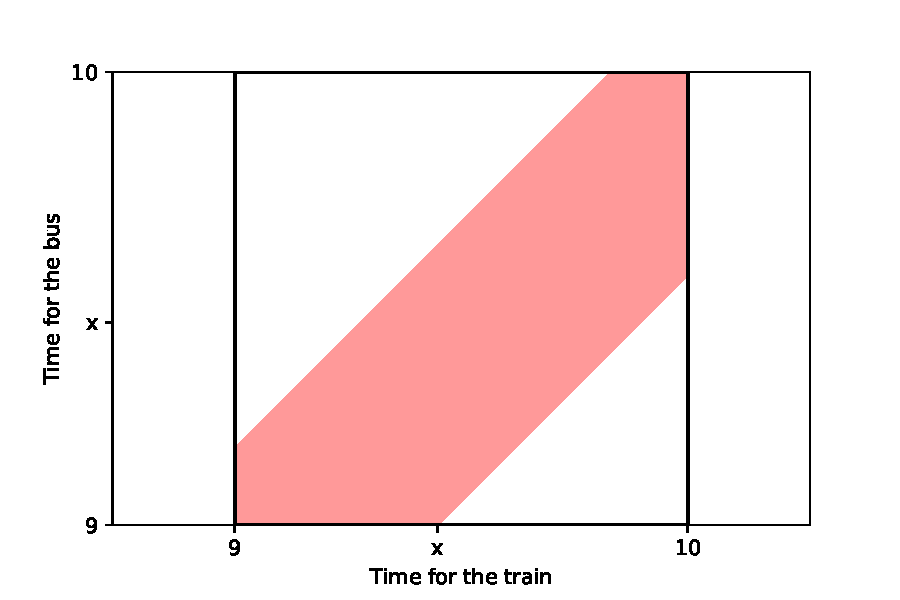
\includegraphics{HW2_Q.pdf}
\end{center}
مساحت ناحیه‌ی هاشور نخورده برابر است با
$$
{25\over 72}+{(1-x)^2\over2}
$$
این مساحت باید برابر $1\over 2$ باشد که در این‌صورت مقدار $x$ برابر 
$
1-{\sqrt{11}\over 6}\approx0.4472 \text{\lr{h}}\approx \text{\rl{27 دقیقه}}
$
 محاسبه می شود.

سوالات 13، 22 و 24 از کتاب مرجع (کتاب 
\lr{
Probability and Statistics
}
 از پاپولیس
)

سوال 13) این مسئله به کمک قانون احتمال کل و استفاده از تعریف احتمال شرطی به راحتی قابل حل است

سوال 22) مشابه سوال 22 از کتاب غیر مرجع.

سوال 24) رشته‌ی لامپ زمانی کار می‌کند که تمام لامپ های آن سالم باشند (تقسیم ولتاژ و خاصیت سری بودن؛ در حالت موازی، کافی است حداقل یکی از لامپ ها کار کند به دلیل تقسیم جریان) در اینصورت خواهیم داشت:
\eqn{
p=(1-0.01)^{50}\approx 0.61
}{}


سوال 1) 
\eqn{
&
P(F)=0.37
\\&
P(M)=0.43
\\&
P(D|M)=0.15
\\&
P(D|F)=0.25
}{}
مطلوب است 
$
P(D|M\cup F)
$.
 در اینصورت داریم
\eqn{
P(D|M\cup F)&=
{P(D\cap[M\cup F])\over P(M\cup F)}
\\&=
{P([D\cap M]\cup [D\cap F])\over P(M)+P(F)}
\\&=
{P(D\cap M)+P(D\cap F)\over P(M)+P(F)}
\\&=
{P(M)P(D|M)+P(F)P(D|F)\over P(M)+P(F)}
\\&=
{0.37\times 0.25+0.43\times 0.15\over 0.8}
\\&\approx 0.20
}{}
این مسئله را به گونه‌ی دیگری نیز می توان حل کرد. از آنجا که به طور کل کودکان در سوال مطرح نمی‌شوند نسبت جمعیت زنان و مردان بزرگسال را به کل بزرگسالان محاسبه می کنیم. به طور کل، 
$
53.75\%
$
 جمعیت بزرگسالان را مردان و
$
46.25\%
$
 را زنان تشکیل می دهند. بنابراین می توان نوشت
\eqn{
&
P(M)=0.5375
\\&
P(F)=0.4625
}{}
و مطلوب 
$
P(D)
$
 خواهد بود؛ در این صورت
\eqn{
P(D)&=
P(D\cap M)+P(D\cap F)
\\&=
P(D|M)P(M)+P(D|F)P(F)
\\&=
0.5375\times 0.15+0.4625\times 0.25
\\&\approx 0.20
}{}

سوال 2)
\eqn{
P(A|B\cap C)&=
{P([A\cap B]\cap [A\cap C])\over P(B)P(C)}
}{}
برای آنکه تساوی ارضا شود، یک شرط کافی مستقل بودن $A\cap B$ و $A\cap C$ است.

سوال 3) کران بالا به وضوح بنا به رابطه‌ی احتمال اجتماع برقرار است. این کران بسیار مهم، \textbf{\rl{کران اجتماع}}
\footnote{
\lr{Union Bound}
}
 نامیده می شود.

برای اثبات کران پایین، ابتدا به دلیل تقارن فرض می کنیم 
$
P(A)\le P(B)
$
. اکنون کافی است مد نظر قرار دهیم که نامساوی های زیر معادلند:
\eqn{
&
P(A)+P(B)-{1\over 4-4P(A)}\le P(A\cup B)
\\& \iff
{1\over 4-4P(A)}\ge P(A\cap B)
\\& \iff
P(A\cap B)(1-P(A))\le {1\over 4}
}{}
از آنجایی که $
P(A\cap B)\le P(A)
$
 و بیشینه مقدار $u-u^2$ به ازای $0<u<1$ در $u={1\over 2}$ رخ می‌دهد، اثبات کامل است

\QA

سوال 1) 

الف) اگر جایگذاری داشته باشیم، پس از برداشتن گلوله‌ی اول به 8 حالت، گلوله‌ی دوم را نیز می توانیم به 8 حالت برداریم. در این صورت از آنجا که ترتیب برداشتن فرقی نمی کند، برداشتن دو گلوله مجموعا به 
$
8\times 8\over 2
$
طریق ممکن است. همچنین اینکه یکی از گلوله ها سفید و دیگری آبی باشد، به 
$
5\times 3
$
راه ممکن است؛ پس احتمال مطلوب برابر است با
$$
P={15\over 32}
$$
\textbf{نکته مهم!!}
ممکن است این گونه برداشت شود که پاسخ اصلی در یک ضریب 2 با پاسخ بالا تفاوت می کند؛ به طور مثال یک راه حل (که البته نادرست است!) به صورت زیر است:

\textbf{
پیشامد اینکه \underline{گلوله‌ی اول سفید و دومی آبی باشد}، 15 حالت متفاوت دارد. چون هر گلوله را به 8 حالت مستقل از دیگری بر می داریم، پاسخ 
$
3\times 5\over 8\times 8
$
می شود.
}

ایراد استدلال بالا این است که رنگ گلوله ها در ترتیب برداشته شدن گلوله ها اثرگذار بوده است. برای اینکه مشکل این استدلال رفع شود، باید پیشامد عکس هم در نظر گرفته شود؛ یعنی حالتی که \underline{گلوله‌ی اول آبی و دومی سفید باشد} تا محور زمان دیده نشود.

نوع دیگر استدلال (درست) چنین است: هنگامی که جایگذاری داشته باشیم، برداشتن گلوله های اول و دوم کاملا از هم مستقل می شود. پس مسئله معادل است با اینکه:

\textit{
دو کیسه داریم که هر یک شامل 5 سفید و 3 آبی است. از هر یک، یک گلوله بر می داریم. با چه احتمالی یکی سفید و دیگری آبی می شود؟
}

مسئله ی فوق، بعد زمان را به فضا تبدیل کرده است؛ یعنی به جای دو بار برداشتن گلوله ها از یک کیسه در زمانهای مختلف، دوتا را از دو کیسه همزمان برداشته ایم. در اینصورت پیشامد اینکه یکی آبی و دیگری سفید باشد، اجتماع دو پیشامد هم احتمال است که هر یک با احتمال
$
15\over 64
$
رخ می دهد؛ پس پاسخ درست 
$
15\over 32
$
است.

ب) اگر جایگذاری مجاز نباشد، دو گلوله را به 
$
\binom{8}{2}=28
$
طریق ممکن می توان برداشت که فقط حالاتی که یکی سفید و دیگری آبی باشد مطلوب است. این حالات مجموعا به 
$
\binom{5}{1}\binom{3}{1}=15
$
طریق ممکن امکان پذیرند؛ پس احتمال مطلوب برابر است با
$$
P={15\over 28}
$$

سوال 2) الف) مکمل این پیشامد، حالتی است که حداکثر یک بار رو ظاهر شود که برابر است با حالاتی که در 10 پرتاب دقیقا 1 رو یا دقیقا صفر رو ظاهر شود (همگی به پشت ظاهر شوند). مجموع احتمالات برابر است با
$$
p'=10\times \left({1\over 2}\right)^9\times \left({1\over 2}\right)^1 +\left({1\over 2}\right)^{10}={11\over 1024}
$$
بنابراین احتمال مطلوب برابر است با
$$
p=1-p'={1013\over 1024}
$$

ب) مشابه قسمت بالا، از آنجا که پرتاب های سکه از هم مستقل هستند، داریم:
$$
p=3\times \left({1\over 2}\right)^2\times \left({1\over 2}\right)^1 +\left({1\over 2}\right)^{3}={1\over2}
$$

پ) احتمال اینکه در پرتاب های زوج نتیجه رو باشد با اینکه پشت باشد، به دلیل تقارن مسئله یکسان است. از طرفی برای محاسبه‌ی احتمال اینکه در پرتاب های زوج نتیجه رو باشد داریم:
$$
p'=\left({1\over 2}\right)^5
$$
بنابراین احتمال مطلوب برابر است با
$$
p=2p'={1\over 16}
$$

سوال 3) این دسته گل را به 
$
\binom{20}{5}=15504
$
راه ممکن می توان برگزید.

الف) اگر دسته گل بخواهد شامل 2 نسترن و 2 بنفشه باشد، باید گل باقیمانده را از بین لاله ها و اقاقیاها به 12 طریق ممکن برداریم. این کار به 
$
\binom{3}{2}\binom{5}{2}\binom{12}{1}=180
$
حالت ممکن امکان پذیر است؛ بنابراین احتمال مطلوب برابر است با
$$
p={180\over 15504}\approx0.01
$$
(اگر فرض کرده اید دسته گل شامل حداقل 2 نسترن یا 2 بنفشه است نیز راه حل مورد قبول است!)

ب) فقط می توان از بین 7 گل بنفشه و اقاقیا انتخاب کرد که این به 
$
\binom{7}{5}=21
$
حالت ممکن است؛ پس:
$$
p={21\over 15504}\approx0.0014
$$
پ) احتمال مطلوب عبارتست از
\[
\begin{split}
p&={1\over 15504}{\binom{10}{2}\binom{5}{1}\binom{3}{1}\binom{2}{1}}
\\&+{1\over 15504}{\binom{10}{1}\binom{5}{2}\binom{3}{1}\binom{2}{1}}
\\&+{1\over 15504}{\binom{10}{1}\binom{5}{1}\binom{3}{2}\binom{2}{1}}
\\&+{1\over 15504}{\binom{10}{1}\binom{5}{1}\binom{3}{1}\binom{2}{2}}
\\&={50\over 323}\approx0.15
\end{split}
\]

سوال 4) الف) هر مجموعه n عضوی شامل $2^n$ زیر مجموعه‌ی متمایز است که 
$
\binom{n}{k}
$
تا از آنها k عضوی اند. پس احتمال مطلوب برابر است با
$$
p={\binom{n}{k}\over 2^n}
$$

ب) از آنجا که مجموع تمام احتمالات فوق برابر 1 است، داریم:
$$
\sum_{k=0}^n{\binom{n}{k}\over 2^n}=1
$$
که معادل گزاره ای است که میخواستیم ثابت کنیم.



سوال 2)

الف)
$$
\binom{n}{m}\left({M\over N}\right)^m\left(1-{M\over N}\right)^{n-m}
$$
ب)
$$
\binom{M}{m}\binom{N-M}{n-m}\over \binom{N}{n}
$$
ج) در این حالت باید داشته باشیم $n=M+2$ در غیر این صورت احتمال برابر صفر است. با این فرض، پس از تمام شدن گلوله های سفید، حتما دو گلوله‌ی سیاه برداشته خواهند شد و این احتمال برابر یک است.
\eqn{
P&=\Pr[\text{\rl{برداشتن دو سیاه}}|\text{\rl{برداشتن تمام سفیدها}}]
\\&=
{
\Pr[\text{\rl{برداشتن دو سیاه}}\cap\text{\rl{برداشتن تمام سفیدها}}]
\over
\Pr[\text{\rl{برداشتن تمام سفیدها}}]
}
\\&=
{
1
}
}{}

سوال 3) این حالت زمانی رخ می دهد که تعداد قدم زدن های به سمت چپ فرد با تعداد قدم زدن های به سمت راست فرد برابر باشد؛ پس اولین شرط زوج بودن $k$ است در غیر این صورت احتمال برابر صفر خواهد بود. با فرض زوج بودن $k$ داریم:
$$
p=\binom{k}{{k\over2}}[p(1-p)]^{k\over 2}
$$

سوال 4) ابتدا، زیرمجموعه ها را با $A$ و $B$ و سپس پیشامد آن را که عدد $i$ در $A$ و $B$ باشد، به ترتیب با $X_i$ و $Y_i$ نمایش می دهیم. در این صورت احتمال زیر مطلوب است:
\eqn{
\Pr&\{\text{\rl{پیشامد قرار نداشتن عدد 1 در هر دو مجموعه}}
\\&\cap
\text{\rl{پیشامد قرار نداشتن عدد 2 در هر دو مجموعه}}
\\&\cap
\text{\rl{پیشامد قرار نداشتن عدد 3 در هر دو مجموعه}}
\\&\cap
\cdots
\\&\cap
\text{\rl{پیشامد قرار نداشتن عدد $n$ در هر دو مجموعه}}
\}
}{}
به زبان ریاضی:
\eqn{
\Pr\left\{\bigcap_{i=1}^{n} \left[X_i\cap Y_i\right]^c\right\}
}{}
به دلیل استقلال می توان نوشت:
\eqn{
\Pr\left\{\bigcap_{i=1}^{n} \left[X_i\cap Y_i\right]^c\right\}&=
\prod_{i=1}^{n}\Pr\left\{\left[X_i\cap Y_i\right]^c\right\}
\\&=
\prod_{i=1}^{n}1-\Pr\left\{X_i\cap Y_i\right\}
\\&=
\prod_{i=1}^{n}1-\Pr\left\{X_i\}\Pr\{Y_i\right\}
\\&=(1-p^2)^n
}{}



سوال 6) احتمال مطلوب عبارتست از:
\eqn{
&\Pr\{
\text{درست بودن پاسخ تمام دانشجویان}|\text{یکسان بودن پاسخ تمام دانشجویان}
\}
\\&=
{
\Pr\{
\text{درست بودن پاسخ تمام دانشجویان}\cap\text{یکسان بودن پاسخ تمام دانشجویان}
\}
\over
\Pr\{
\text{یکسان بودن پاسخ تمام دانشجویان}
\}
}
}{}
پیشامد آن که تمام دانشجویان مستقل از هم به پاسخ درست برسند، حالت خاصی از کوشش مکرر و احتمال آن برابر $p^n$ است. احتمال آن که دانشجویان به پاسخ یکسانی برسند طبق قاعده‌ی احتمال کل برابر احتمال پاسخ یکسان در دو حالت پاسخ درست یا نادرست است. احتمال آن که تمام دانشجویان به پاسخ نادرست رسیده باشند برابر $(1-p)^n$ و در نتیجه احتمال مطلوب برابر 
$$
{p^n\over p^n+(1-p)^n}={1\over 1+\left(1-{1\over p}\right)^n}
$$
خواهد بود. نسبت $1-{1\over p}$ را می توان معیاری از سختی سوال ارزیابی کرد. در حقیقت هر چه سوال به تعبیر ریاضی آن ``سخت تر'' باشد، احتمال درست پاسخ دادن تمام دانشجویانی که به پاسخ یکسان رسیده اند کمتر است. به علاوه هر چه تعداد دانشجویان بیشتری پس از امتحان به یک پاسخ رسیده باشند، احتمال آن که همه‌ی آنها اشتباه کنند بیشتر می شود. این وضعیت را می‌توان در نمودار زیر مشاهده کرد:
\begin{center}
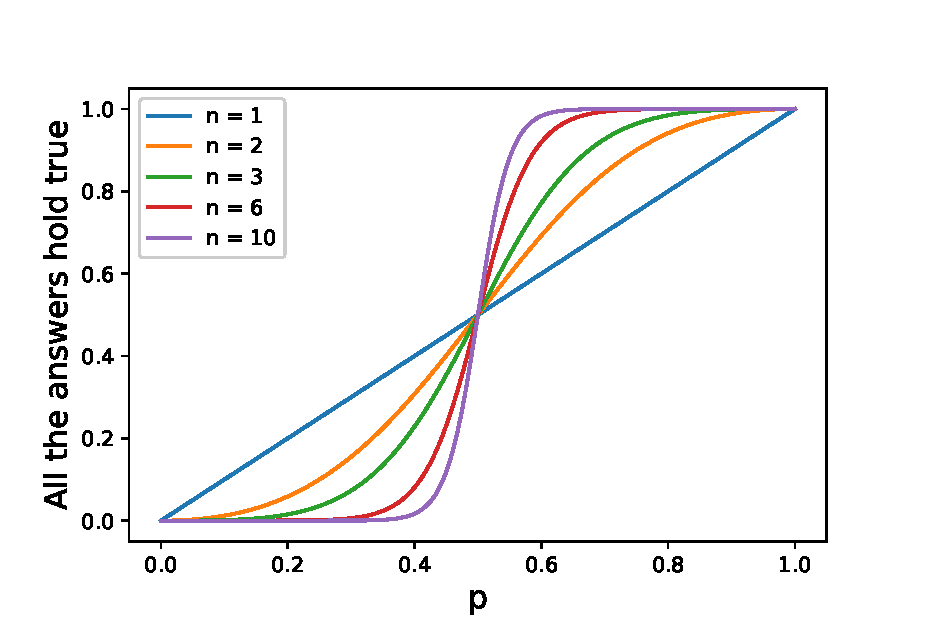
\includegraphics{HW3_Q6.eps}
\end{center}

\QA

سوال 1)
\[
\begin{split}
&\Pr\{\text{ابتلا به کرونا}|\text{ماسک زدن}\}=0.15
\\&\Pr\{\text{ابتلا به کرونا}|\text{ماسک نزدن}\}=0.7
\\&\Pr\{\text{ماسک زدن}\}=0.05
\end{split}
\]

\[
\begin{split}
\Pr\{\text{ابتلا به کرونا}\}&=
\Pr\{\text{ابتلا به کرونا}|\text{ماسک زدن}\}
\Pr\{\text{ماسک زدن}\}
\\&+
\Pr\{\text{ابتلا به کرونا}|\text{ماسک نزدن}\}
\Pr\{\text{ماسک نزدن}\}
\\&=0.7\times 0.95+0.15\times0.05=67.25\%
\end{split}
\]

سوال 2) 
$$
\Pr\{\text{هردو زوج}\}=\Pr\{\text{هردو زوج}\}={9\over 36}={1\over 4}\implies \Pr\{\text{جمع زوج}\}={1\over2}=0.5
$$

ب)
$$
\Pr\{\text{جمع بیشتر از 8}|\text{جمع زوج}\}=
{\Pr\{\text{جمع بیشتر از 8}\cap\text{جمع زوج}\}\over
\Pr\{\text{جمع زوج}\}
}
=
{{4\over 36}\over {1\over 2}}={2\over 9}\approx0.22
$$

سوال 3) 

\textbf{راه 1}

 اگر عناصر 1 و 2 را که در هر دو زیر مجموعه هستند کنار بگذاریم، سایر اعضا را به 
$
3^{n-2}
%\binom{2^{n-2}}{2}
$
طریق ممکن می توان بین دو زیرمجموعه پخش کرد. از طرفی برای آنکه اشتراک دو زیر مجموعه برابر 
$
\{1,2\}
$
باشد و اعضای 
$
3,4,5
$
داخل یکی از زیرمجموعه ها بیفتند، باید در هنگام انتخاب سایر اعضای زیرمجموعه ها از بین اعضای 
$
\{5,\cdots,n\}
$
ابتدا هر عضو مجموعه‌ی بالا را در نظر بگیریم. هر عضو سه حالت دارد: یا فقط داخل زیرمجموعه‌ی 1 است؛ یا فقط داخل زیر مجموعه‌ی 2 است و یا در هیچ یک از زیر مجموعه ها نیست. بنابراین این کار به 
$
3^{n-5}
$
طریق ممکن امکان پذیر می شود و احتمال مطلوب برابر است با
$$
{3^{n-5}\over 3^{n-2}}={1\over 27}
$$

\textbf{راه 2}

از آنجا که 1 و 2 در هر دو زیرمجموعه هستند، می توان آنها را نادیده گرفت و سایر اعضای هر دو زیرمجموعه را از اعضای 
$
\{3,4,\cdots,n\}
$
برگزید. با این شرط، تعداد کل حالاتی که می توان دو زیر مجموعه را برگزید عبارتست از اینکه ابتدا k عضو برداریم و سپس این k عضو را بین دو زیرمجموعه پخش کنیم؛ یعنی
$$
\sum_{k=0}^{n-2}\binom{n-2}{k}2^{k}=3^{n-2}
$$
تعداد حالاتی که یکی از زیر مجموعه های شامل عناصر $\{3,4,5\}$ باشد، این است که عناصر معلوم الحال را (یعنی $\{1,2,3,4,5\}$) در نظر بگیریم و سپس سایر اعضا را از بین 
$
\{6,\cdots,n\}
$
برگزینیم. این کار به طریق مشابه به 
$$
\sum_{k=0}^{n-5}\binom{n-5}{k}2^{k-1}=3^{n-5}
$$
امکان پذیر است؛ پس احتمال مطلوب می شود:
$$
{\sum_{k=0}^{n-5}\binom{n-5}{k}2^{k-1}\over
\sum_{k=0}^{n-2}\binom{n-2}{k}2^{k-1}
}={1\over 27}
$$

سوال 4) پیشامد معیوب بودن لامپ را با $C$ و انتخاب جعبه‌ی $i$ ام را با $B_i$ نشان می دهیم. در این صورت:

الف)
$$
P(C)=\sum_{i=1}^{3}P(C|B_i)P(B_i)
={1\over 3}\left({3\over 1000}+{3\over 10}+{0\over 3000}\right)=0.101
$$

ب)
$$
P(B_2|C)={P(B_2\cap C)\over P(C)}={P(C|B_2)P(B_2)\over P(C)}
={{3\over 10}\times {1\over 3}\over {101\over 1000}}={100\over 101}\approx0.99
$$

پ)
\[
\begin{split}
P(B_1\cup B_2|C')&=
{P([B_1\cup B_2]\cap C')\over P(C')}
\\&=
{P([B_1\cap C']\cup [B_2\cap C'])\over P(C')}
\\&=
{P(B_1\cap C')+P(B_2\cap C')\over P(C')}
\\&=
{P(C'|B_1)P(B_1)+P(C'|B_2)P(B_2)\over P(C')}
\\&=
{{1\over 3}\left({997\over 1000}+{7\over 10}\right)
\over
1-0.101
}
\approx0.63
\end{split}
\]

سوال 5)

$$
P(P_1|B)={P(P_1\cap B)\over P(B)}={P(B|P_1)P(P_1)\over P(B)}
={{20\over 100}\times{100\over 100+1000}\over {70\over 1100}}={2\over 7}\approx 0.29
$$

$$
P(P_2\cap B'|F)={P(P_2\cap B'\cap F)\over P(F)}
={{630\over 1100}\over {690\over 1100}}={21\over 23}\approx 0.91
$$

$$
P(B|M)={P(B\cap M)\over P(M)}={{40\over 1100}\over {410\over 1100}}
={4\over 41}\approx 0.10
$$

\QA

سوال 1)

الف) از آنجا که برای $n<a$ و $n>b$ به ترتیب داریم
$
F(n)=0
$
 و 
$
F(n)=1
$
 در نتیجه می توان نوشت:
$$
f(n)=\begin{cases}
{1\over b-a+1}&,\quad a\le n\le b
\\0&,\quad\text{\rl{
در غیر این صورت
}} 
\end{cases}
$$
بنابراین
\eqn{
\sum_{n=-\infty}^\infty nf(n)&=\sum_{n=a}^b {n\over b-a+1}
\\&=
\sum_{n=1}^b {n\over b-a+1}-
\sum_{n=1}^{a-1} {n\over b-a+1}
\\&={b^2+b-a^2+a\over 2(b-a+1)}
\\&={(b+a)(b-a+1)\over 2(b-a+1)}
\\&={b+a\over 2}
}{}
ب) 
\eqn{
f(n)=A^n-A^{n+1}=A^n(1-A)\quad,\quad n\ge 0
}{}
در نتیجه 
\eqn{
\sum_{n=-\infty}^\infty nf(n)&=
\sum_{n=0}^\infty nA^n(1-A)
\\&=
\sum_{n=1}^\infty nA^n(1-A)
\\&=
A(1-A)\sum_{n=1}^\infty nA^{n-1}
\\&=
A(1-A){d\over dA}\sum_{n=1}^\infty A^{n}
\\&=
A(1-A){d\over dA}{A\over 1-A}
\\&=
{A\over 1-A}
}{}
سوال 2)

الف)
\eqn{
f(x)=
{1\over \lambda}e^{-{1\over \lambda}x}\quad,\quad x>0
}{}
در نتیجه
\eqn{
\int_{-\infty}^\infty xf(x)dx&=\int_0^\infty {x\over \lambda}e^{-{1\over \lambda}x}dx
\\&=
-{x}e^{-{1\over \lambda}x}\Big|_{0}^{\infty}+
\int_0^\infty e^{-{1\over \lambda}x}dx
\\&=
\int_0^\infty e^{-{1\over \lambda}x}dx
\\&=
-\lambda e^{-{1\over \lambda}x}\Big|_0^\infty
\\&=\lambda
}{}
ب)
\[
f(x)={1\over b-a}\quad,\quad a<x<b
\]
بنابراین
\eqn{
\int_{-\infty}^\infty xf(x)dx&=\int_a^b {x\over b-a}dx
\\&={b^2-a^2\over 2(b-a)}
\\&={b+a\over 2}
}{}
پ)
\eqn{
f(x)&={1\over \sqrt{2\pi\sigma^2}}\exp\left({(t-\mu)^2\over 2\sigma^2}\right)\Big|_{t=x}-
{1\over \sqrt{2\pi\sigma^2}}\exp\left({(t-\mu)^2\over 2\sigma^2}\right)\Big|_{t=-\infty}
\\&={1\over \sqrt{2\pi\sigma^2}}\exp\left({(x-\mu)^2\over 2\sigma^2}\right)
}{}
بنابراین
\eqn{
\int_{-\infty}^\infty xf(x)dx&=
{1\over \sqrt{2\pi\sigma^2}}
\int_{-\infty}^\infty
x\cdot\exp\left({(x-\mu)^2\over 2\sigma^2}\right)
dx
\\&=
{1\over \sqrt{2\pi\sigma^2}}
\int_{-\infty}^\infty
(x-\mu+\mu)\cdot\exp\left({(x-\mu)^2\over 2\sigma^2}\right)
dx
\\&=
\underbrace{{1\over \sqrt{2\pi\sigma^2}}
\int_{-\infty}^\infty
(x-\mu)\cdot\exp\left({(x-\mu)^2\over 2\sigma^2}\right)
dx}_{\triangleq I_1}
\\&
+\underbrace{{1\over \sqrt{2\pi\sigma^2}}
\int_{-\infty}^\infty
\mu\cdot\exp\left({(x-\mu)^2\over 2\sigma^2}\right)
dx}_{\triangleq I_2}
}{}
انتگرال $I_1$ برابر است با $
{1\over \sqrt{2\pi\sigma^2}}
\int_{-\infty}^\infty
w\cdot\exp\left({w^2\over 2\sigma^2}\right)
dw
$
 که همگرا و برابر صفر است؛ زیرا این انتگرال، انتگرال یک تابع فرد را روی بازه‌ی متقارنی نشان می دهد به علاوه جمله ی نمایی میرا شونده باعث کاهش سریع تابع تحت انتگرال می گردد. برای انتگرال $I_2$ نیز با توجه به تابع $F(x)$ تعریف شده در صورت سوال می توان نوشت:
\eqn{
I_2=\mu{1\over \sqrt{2\pi\sigma^2}}
\int_{-\infty}^\infty
\exp\left({(x-\mu)^2\over 2\sigma^2}\right)
dx
=\mu F(\infty)=\mu
}{}
در مجموع خواهیم داشت:
\eqn{
\int_{-\infty}^\infty xf(x)dx=\mu
}{}
سوال 3) 

متغیر تصادفی برنولی، یک متغیر تصادفی دو مقداره است که تنها مقادیر صفر و یک را می پذیرد. به طور مثال برای متغیر تصادفی برنولی $X$ داریم
$$
\Pr\{X=1\}=p
$$
از آنجا که عملگر این قسمت یک \text{\lr{xor}} (یا جمع به پیمانه‌ی 2) است، متغیر تصادفی $Z$ نیز دو مقداره و دارای توزیع برنولی خواهد بود.
\eqn{
\Pr\{Z=1\}&=\Pr\{X\oplus Y\mod 2=1\}
\\&=\Pr\{X\text{\lr{xor}} Y=1\}
\\&=\Pr\{X=1,Y=0\text{\rl{ یا }}X=0,Y=1\}
\\&=\Pr\{X=1,Y=0\}+\Pr\{X=1,Y=0\}
\\&=\Pr\{X=1\}\Pr\{Y=0\}+\Pr\{X=0\}\Pr\{Y=1\}
\\&={1\over 2}\cdot (1-p)+{1\over 2}\cdot p
\\&={1\over 2}
}{}
سوال 4)

 با توضیحاتی مشابه سوال قبل، به سادگی دیده می شود که متغیر تصادفی $Z$ دو مقداره و دارای توزیع برنولی خواهد بود.
\eqn{
\Pr\{Z=1\}&=\Pr\{XY=1\}
\\&=\Pr\{X=1,Y=1\}
\\&=\Pr\{X=1\}\Pr\{Y=1\}
\\&={1\over 2}p
}{}
سوال 5)

متغیر تصادفی $X$ حاصل $n_1$ کوشش برنولی مستقل با پارامتر احتمالاتی $p$ و متغیر تصادفی $Y$ حاصل $n_2$ کوشش برنولی مستقل با پارامتر احتمالاتی $p$ است؛ در نتیجه می توان متغیر های تصادفی $X$ و $Y$ را به مانند تعداد شیرهای رو آمده در پرتاب به ترتیب $n_1$ و $n_2$ بار سکه‌ی ناسالم تعبیر نمود. با این تعبیر، متغیر تصادفی $X+Y$ تعداد شیرها را در $n_1+n_2$ بار پرتاب همان سکه‌ی ناسالم نشان می دهد؛ به عبارت دیگر فرقی نمی کند که ابتدا سکه را $n_1$ بار پرتاب کرده و تعداد شیر ها را یادداشت کنیم، سپس با تعداد شیرها در $n_2$ بار پرتاب جمع بزنیم یا از ابتدا سکه را $n_1+n_2$ بار پرتاب کنیم و سپس تعداد شیرها را یادداشت کنیم. این عدم تفاوت، به دلیل مستقل بودن پرتاب هاست و در صورت مستقل نبودن پرتاب ها، استدلال های فوق معتبر نخواهند بود.

الف) فضای نمونه عبارتست از مجموعه‌ی تمام برآمدها(رخدادها)یی که می‌توانند در یک مسئله‌ی احتمالاتی رخ دهند. به طور مثال، فضای نمونه‌ی پرتاب تاس،
$
\{1,2,3,4,5,6\}
$
است.


ب) به هر زیرمجموعه از فضای نمونه، یک پیشامد یا واقعه گفته می‌شود. در پرتاب تاس، واقعه‌ی روآمدن عدد زوج معادل مجموعه‌ی 
$
\{2,4,6\}
$
است.

پ) به هر زیرمجموعه‌ی تک عضوی از فضای نمونه، یک پیشامد ساده یا برآمد گفته می‌شود. در پرتاب تاس، 6 برآمد وجود دارد.

\QA

در صورتی که فضای نمونه متناهی باشد، پاسخ مثبت است؛ زیرا هر برآمد دارای احتمال مثبت است و در نتیجه، احتمال رخداد هر زیرمجموعه کمتر از 1 خواهد بود. در حالتی که فضای نمونه نامتناهی باشد، حذف یک برآمد با احتمال رخداد صفر از فضای نمونه، تغییر در احتمال آن ایجاد نمی‌کند. به طور مثال، فرض کنید بخواهیم عددی حقیقی را به تصادف کامل از بازه‌ی 
$
[0,1]
$
برگزینیم. در این صورت، احتمال اینکه این عدد برابر $0.5$ نباشد برابر 1 است.

\QA

الف)
\eqn{
A\times B=\{
&
(\text{H},1),
(\text{H},2),
(\text{H},3),
(\text{H},4),
(\text{H},5),
(\text{H},6),
\\&
(\text{T},1),
(\text{T},2),
(\text{T},3),
(\text{T},4),
(\text{T},5),
(\text{T},6)
\}
}

این مجموعه، فضای نمونه‌ی آزمایش پرتاب توأم تاس و سکه است (``یک سکه و یک تاس را به طور همزمان پرتاب میکنیم...'').

ب) به طور مثال
\eqn{
&S_1=\{(\text{T},2),(\text{H},5),(\text{T},6)\}
\\&S_2=\{(\text{H},2),(\text{T},5),(\text{H},6)\}
}

نمی‌توان همین کار را برای زیرمجموعه‌های 7 عضوی تکرار کرد؛ چرا که طبق اصل لانه‌ی کبوتری، حداقل دو عضو تکراری در این دو زیرمجموعه وجود خواهد داشت.



\QA

می‌دانیم
\eqn{
P\left\{
A\cap(B\cup C)
\right\}
&=
P\left\{
[A\cap B]\cup[A\cap C]
\right\}
}
از طرفی
\eqn{
[A\cap B]\cap[A\cap C]
=
A\cap B\cap C
=
A\cap [B\cap C]
=
A\cap \emptyset
=
\emptyset
}
بنابراین طبق اصل سوم کولموگروف،
\eqn{
P\left\{
A\cap(B\cup C)
\right\}
&=
P\left\{
[A\cap B]\cup[A\cap C]
\right\}
\\&=
P\left\{
A\cap B
\right\}
+
P\left\{
A\cap C
\right\}
.
}

اگر پیشامدهای ابتلا به کرونا و آنفلوآنزا را به ترتیب با 
$
A
$
و
$
B
$
نشان دهیم، طبق فرض مسئله داریم
\eqn{
&P(A)=0.07,
\\&P(B)=0.19,
\\&P(A\cup B)=0.2
.
}
در این صورت

الف) خواسته‌ی مسئله، 
$
P(A\cap B)
$
است که برابر است با
$$
P(A\cap B)=P(A)+P(B)-P(A\cup B)=0.07+0.19-0.2=0.06
$$

ب) مطلوبست 
$
P(A-B)
$
. در این صورت
$$
P(A-B)=P(A)-P(A\cap B)=0.07-0.06=0.01.
$$

\QA

الف)
$$
P(A)=P(2)+P(3)+P(5)+P(7)=0.1+0.1+0.1+0.1=0.4
$$

ب)
\eqn{
&A-B=\{2\}
\\&A\cap B=\{3,5,7\}
\\&\implies
\\&P(A-B)=0.1
\\&P(A\cap B)=0.3
}

پ) داریم
\eqn{
&P(A-B)=0.1
\\&P(A)=0.4
\\&P(A\cap B)=0.3
}
بنابراین درستی رابطه‎‌ی زیر مشاهده می‌شود:
\eqn{
P(A-B)=P(A)-P(A\cap B).
}
علت درستی این رابطه آن است که دو مجموعه‌ی 
$
A-B
$
و
$
A\cap B
$
ناسازگارند؛ در نتیجه طبق اصل سوم کولموگروف
$$
P(A\cap B)+P(A-B)=P([A\cap B]\cup[A-B])=P(A).
$$

\QA
نامساوی سمت راست به سادگی از 
$$
P(A\cap B)=P(A)+P(B)-P(A\cup B)
$$
و 
$
P(A\cap B)\ge 0
$
نتیجه می‌شود. برای نامساوی سمت چپ باید اثبات کنیم
\eqn{
P(A\cap B)\le\frac{1}{4\max\{1-P(A),1-P(B)\}}
}
به دلیل تقارن مسئله، فرض می‌کنیم
$
P(A)\ge P(B)
$.
در نتیجه
\eqn{
P(A\cap B)\le\frac{1}{4[1-P(B)]}.
}
از طرفی
\eqn{
&(\frac{1}{2}-P(B))^2\ge0\implies
\\&
4P^2(B)-4P(B)+1\ge0\implies
\\&
1\ge 4P(B)-4P^2(B)\implies
\\&
1\ge 4P(B)[1-P(B)]\implies
\\&
P(B)\le\frac{1}{4[1-P(B)]}.
}
همچنین می دانیم 
$
A\cap B\ \ \ \subseteq\ \ \  B
$
. در نتیجه
\eqn{
P(A\cap B)\le P(B)\le\frac{1}{4[1-P(B)]}
}
و اثبات کامل می شود
$
\blacksquare
$

اگر کتابهای هم نوع متمایز باشند، اینکه مثلا دو کتاب رمان نسبت به هم در چه موقعیتی قرار میگیرند مهم است. با این فرض، تمام کتابها متمایزند و مجموع حالات مطلوب،
$
(3+2+4)!=9!
$
خواهد بود.

اگر تمام کتابهای هم نوع نامتمایز باشند، در این صورت دو حالت که دو کتاب رمان در دو موقعیت متفاوت نسبت به هم باشند (مثلا رمان بینوایان سمت چپ یا راست رمان گوژپشت نتردام باشد!)، یکبار شمرده می‌شوند. ترتیب کتابهای فیزیک و روانشناسی نیز به 
$
3!
$
و
$
4!
$
حالت مختلف تعیین می شود. در این صورت، تعداد کل حالات مطلوب برابر
$
\frac{9!}{3!\times 2!\times 4!}
$
خواهد بود.

\QA

این دسته گل می تواند شامل حالات زیر باشد:

- 3 بنفشه

- 2 بنفشه و 1 رز

- 2 بنفشه و 1 اقاقیا

- 1 بنفشه و 2 رز

- 1 بنفشه و 2 اقاقیا

- 1 بنفشه، 1 رز و 1 اقاقیا

- 3 رز

- 2 رز و 1 اقاقیا

- 1 رز و 2 اقاقیا

در نتیجه، مجموع کل حالات مطلوب عبارتست از
\eqn{
&
\binom{3}{3}+
\binom{3}{2}\binom{4}{1}+
\binom{3}{2}\binom{2}{1}+
\binom{3}{1}\binom{4}{2}+
\binom{3}{1}\binom{2}{2}+
\\&
\binom{3}{1}\binom{2}{1}\binom{4}{1}+
\binom{4}{3}+
\binom{4}{2}\binom{2}{1}+
\binom{4}{1}\binom{2}{2}=
\\&
1+12+6+18+3+24+4+12+4=84.
}{}

\QA

در حل مسائلی که با افراد سروکار دارند، اگر مسئله از نوع کلان نباشد (مانند شیوع افسردگی در یک جامعه که به طور نسبی، به تعداد افراد مربوط است نه به تک تک آنها)، باید افراد را متمایز دانست. مسئله‌ی پیش رو چنین حالتی دارد. به دلیل اینکه نشست در یک میزگرد اتفاق می افتد، ابتدا یک نفر (مثلا مدیرعامل) را در یک صندلی می‌نشانیم و سپس حالات نشستن سایر افراد را بررسی می کنیم (چرا؟).

الف)اگر هر دو منشی کنار هم باشند، ابتدا هر دو نفر را یک نفر (به نام دو-منشی) به حساب می آوریم و تعداد حالات حاصله را می‌شماریم. سپس تعداد حالات را در تعداد ترتیبات نشستن دو منشی نسبت به هم ضرب می کنیم. با این رویکرد، دو-منشی دو صندلی کنار هم اختیار می‌کند که معادل این است که یک صندلی به او اختصاص داده و از تمام صندلی ها 1 واحد کم کنیم. در این صورت، دو-منشی و سایر اعضا (به غیر از مدیرعامل)، باید 7 صندلی از 9 صندلی باقیمانده را تصاحب کنند. این کار، به دلیل تمایز اعضا، به 
$
\binom{9}{7}\times 7!
$
طریق ممکن امکان پذیر است. چون دو-منشی شامل دو حالت ترتیب نشستن منشی ها نسبت به هم است، تعداد کل حالات ممکن برابر 
$
2\times 7!\times \binom{9}{7}=362880
$
خواهد بود.

ب) در این حالت باید تمام اعضای هیئت مدیره، 5 صندلی از 8 صندلی باقیمانده (غیرمجاور با مدیرعامل و خود مدیرعامل) را به 
$
5!\times \binom{8}{5}=6720
$
طریق تصاحب کنند. سپس منشی ها و حسابدار می‌توانند 3 صندلی از 5 صندلی باقیمانده را به 
$
3!\times\binom{5}{3}=60
$
راه انتخاب کنند. تعداد کل حالات طبق اصل ضرب برابر 
$
403200
$
خواهد بود.

پ) حسابدار به دو حالت کنار مدیرعامل می‌نشیند و تمام اعضای هیئت مدیره (به جز مدیرعامل) را که کنار هم می‌نشینند، یک نفر به نام پنج-مدیر در نظر می‌گیریم. پنج-مدیر، 5 صندلی کنار هم انتخاب می‌کند که در این صورت، معادلأ با 3 نفر روبرو هستیم که باید بر روی 5 صندلی بنشینند. مشابه بخش الف و به دلیل تمایز منشی ها و اعضای هیئت مدیره، تعداد کل حالات مطلوب برابر است با
$
\binom{5}{3}\times 3!\times 5!\times 2=14400
$.



\QA

الف) طبق اصل ضرب، ابن کار به 
$
7\times 10=70
$
طریق ممکن (بدون احتساب ترتیب) و 140 طریق ممکن (با احتساب ترتیب) امکان پذیر است.

ب) تعداد کل حالات ممکن برای برداشتن 2 توپ، برابر 
$
\binom{17}{2}=136
$
است و در نتیجه، احتمال مطلوب برابر 
$
\frac{70}{136}
$
خواهد بود.

پ) از آنجا که فقط یک توپ آبی مشخص و یک توپ قرمز مشخص مد نظر ماست، تنها به یک حالت می‌توانیم این دو توپ را برداریم (دقت کنید چه ترتیب انتخاب را محسوب کنیم چه نکنیم، تعداد حالات را عوض می‌کند ولی در مقدار احتمال تأثیری ندارد). در نتیجه احتمال مطلوب برابر 
$
\frac{1}{136}
$
خواهد بود.

ت) خیر؛ چرا که متمایز کردن توپ ها (به کمک شماره گذاری آنها)، جزو مطلوبات مسئله نبوده است.

\QA

ب) برداشتن دو توپ با جایگذاری، مانند این است که دو توپ از دو کیسه‌ی کاملا مشابه (یک توپ از هر کیسه) برداریم. از آنجا که ترتیب انتخاب نباید مهم باشد، حالتی که توپ کیسه‌ی اول قرمز و توپ کیسه‌ی دوم آبی است، هم ارزند و باید هر دو شمرده شوند. در این صورت، تعداد حالات برداشتن دو توپ به این روش که یکی آبی و دیگری قرمز باشد،
$
140
$
تا است و همچنین، این دو توپ به 
$
{17\times 17}=289
$
حالت ممکن برداشته می‌شوند (اگر ترتیب انتخاب مهم نباشد). در نتیجه، احتمال مطلوب برابر 
$
\frac{140}{289}
$
خواهد بود.

پ) به طریق مشابه قبل، دو حالت امکان پذیر است که توپ های شماره دار خاصی از هر رنگ برداشته شوند. در نتیجه، احتمال مطلوب برابر 
$
\frac{2}{289}
$
خواهد بود.

ت) خیر. دلیل مشابه است؛ زیرا متمایز بودن توپها جزو مطلوبات مسئله نبوده است.

\QA

مربع زیر را در نظر بگیرید:
\begin{figure}[h]
\centering
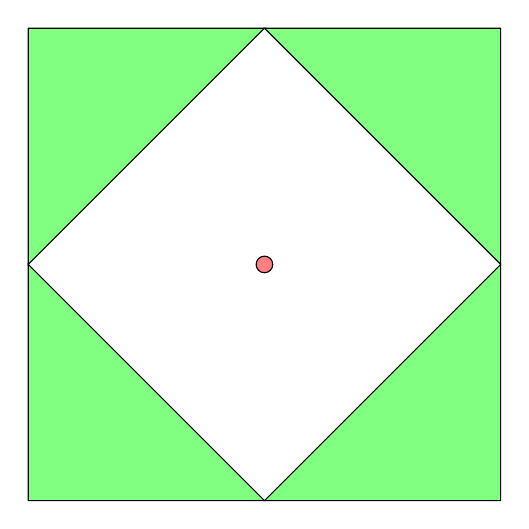
\begin{tikzpicture}
\draw (0,0)--(0,6)--(6,6)--(6,0)--(0,0);
\filldraw[fill=green!50!white] (0,0)--(0,3)--(3,0)--(0,0);
\filldraw[fill=green!50!white] (6,6)--(6,3)--(3,6)--(6,6);
\filldraw[fill=green!50!white] (0,6)--(0,3)--(3,6)--(0,6);
\filldraw[fill=green!50!white] (6,0)--(6,3)--(3,0)--(6,0);
\filldraw[fill=red!50!white] (3,3) circle (3pt);
\end{tikzpicture}
\end{figure}
اگر نقطه‌ی تصادفی مسئله، در یکی از نواحی سبز بیفتد، فاصله‌ی آن تا مرکز مربع از فاصله‌ی آن تا حداقل یکی از رئوس مربع بیشتر است. از آنجا که نواحی سبز، نصف مساحت مربع را اشغال می‌کنند در نتیجه احتمال مطلوب برابر 
$
\frac{1}{2}
$
خواهد بود.


\QA

الف) با قرار دادن رخ سفید، دقیقا 
$
2\times 8-2=14
$
خانه در معرض حمله‌ی رخ سفید قرار می‌گیرند (این موضوع، مستقل از مکان قرارگیری رخ سفید است). در نتیجه پیشامد مطلوب آن است که رخ سیاه، در یکی از این خانه‌ها قرار گیرد که این امر، با احتمال 
$
\frac{14}{63}=\frac{2}{9}
$
رخ می‌دهد.

ب) برای مات شدن شاه سفید، حتما باید حداقل یکی از رخ های سیاه، گوشه‌ای را که شاه سفید در آن قرار دارد تهدید کند. در نتیجه یکی از رخ ها باید در یکی از 14 خانه‌ی ممکن قرار داشته باشد. به دلیل تقارن مسئله، فرض می‌کنیم یک رخ سیاه، در پایینی ترین ردیف قرار دارد.

هنگامی که یک رخ، ردیف یا ستونی که شامل شاه است را تهدید می‌کند، برای مات کردن شاه، رخ دیگر باید ردیف یا ستون دیگری را که شاه می‌تواند حرکت کند، به طور کامل تهدید کند (شکل 2؛ دایره‌ی قرمز و مثل سبز به ترتیب نشان دهنده‌ی شاه سفید و رخ سیاه هستند). از طرفی، یکی از رخ ها نمی تواند خانه‌ی سیاه بالای شاه را اشغال کند؛ زیرا شاه با زدن آن مهره، از کیش و مات فرار میکند. همچنین اگر یکی از رخ‌ها در خانه‌ی مجاور شاه باشد، رخ دیگر نیز باید دقیقأ بالای آن قرار بگیرد و بالعکس؛ در غیر اینصورت، شاه با زدن رخ کنار خود یا رخی که در خانه‌ی همسایه‌ی قطری شاه قرار دارد، از کیش فرار می‌کند. در نتیجه، آرایش 2 تایی رخ ها به 
$
6\times 6+1=37
$
طریق ممکن امکان پذیر است. به دلیل تقارن، مات شدن می‌تواند به صورت ستونی نیز زخ دهد؛ در نتیجه تعداد کل حالات مطلوب برابر 
$
2\times 37=74
$
و احتمال مطلوب برابر 
$
\frac{74}{\binom{63}{2}}=\frac{74}{1953}
$
خواهد بود.

\begin{figure}[h]
\centering
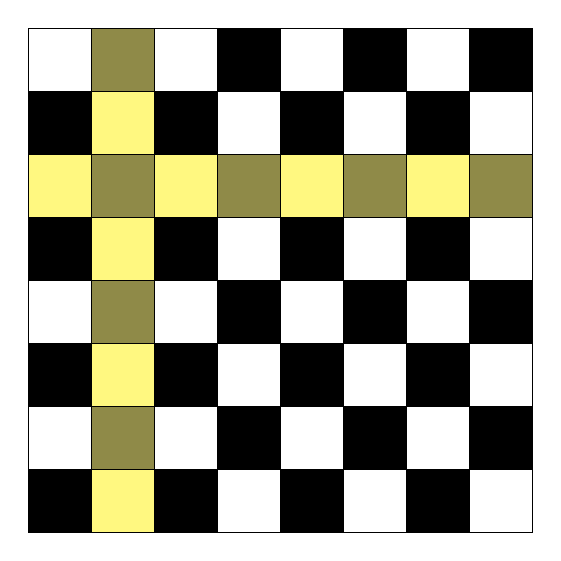
\begin{tikzpicture}
\filldraw[fill=black](-3.2,-3.2)--(-2.4000000000000004,-3.2)--(-2.4000000000000004,-2.4000000000000004)--(-3.2,-2.4000000000000004)--(-3.2,-3.2);
\filldraw[fill=white](-3.2,-2.4000000000000004)--(-2.4000000000000004,-2.4000000000000004)--(-2.4000000000000004,-1.6000000000000003)--(-3.2,-1.6000000000000003)--(-3.2,-2.4000000000000004);
\filldraw[fill=black](-3.2,-1.6)--(-2.4000000000000004,-1.6)--(-2.4000000000000004,-0.8)--(-3.2,-0.8)--(-3.2,-1.6);
\filldraw[fill=white](-3.2,-0.8)--(-2.4000000000000004,-0.8)--(-2.4000000000000004,0.0)--(-3.2,0.0)--(-3.2,-0.8);
\filldraw[fill=black](-3.2,0.0)--(-2.4000000000000004,0.0)--(-2.4000000000000004,0.8)--(-3.2,0.8)--(-3.2,0.0);
\filldraw[fill=yellow!50!white](-3.2,0.8)--(-2.4000000000000004,0.8)--(-2.4000000000000004,1.6)--(-3.2,1.6)--(-3.2,0.8);
\filldraw[fill=black](-3.2,1.6)--(-2.4000000000000004,1.6)--(-2.4000000000000004,2.4000000000000004)--(-3.2,2.4000000000000004)--(-3.2,1.6);
\filldraw[fill=white](-3.2,2.4000000000000004)--(-2.4000000000000004,2.4000000000000004)--(-2.4000000000000004,3.2)--(-3.2,3.2)--(-3.2,2.4000000000000004);
\filldraw[fill=yellow!50!white](-2.4000000000000004,-3.2)--(-1.6000000000000003,-3.2)--(-1.6000000000000003,-2.4000000000000004)--(-2.4000000000000004,-2.4000000000000004)--(-2.4000000000000004,-3.2);
\filldraw[fill=yellow!50!black](-2.4000000000000004,-2.4000000000000004)--(-1.6000000000000003,-2.4000000000000004)--(-1.6000000000000003,-1.6000000000000003)--(-2.4000000000000004,-1.6000000000000003)--(-2.4000000000000004,-2.4000000000000004);
\filldraw[fill=yellow!50!white](-2.4000000000000004,-1.6)--(-1.6000000000000003,-1.6)--(-1.6000000000000003,-0.8)--(-2.4000000000000004,-0.8)--(-2.4000000000000004,-1.6);
\filldraw[fill=yellow!50!black](-2.4000000000000004,-0.8)--(-1.6000000000000003,-0.8)--(-1.6000000000000003,0.0)--(-2.4000000000000004,0.0)--(-2.4000000000000004,-0.8);
\filldraw[fill=yellow!50!white](-2.4000000000000004,0.0)--(-1.6000000000000003,0.0)--(-1.6000000000000003,0.8)--(-2.4000000000000004,0.8)--(-2.4000000000000004,0.0);
\filldraw[fill=yellow!50!black](-2.4000000000000004,0.8)--(-1.6000000000000003,0.8)--(-1.6000000000000003,1.6)--(-2.4000000000000004,1.6)--(-2.4000000000000004,0.8);
\filldraw[fill=yellow!50!white](-2.4000000000000004,1.6)--(-1.6000000000000003,1.6)--(-1.6000000000000003,2.4000000000000004)--(-2.4000000000000004,2.4000000000000004)--(-2.4000000000000004,1.6);
\filldraw[fill=yellow!50!black](-2.4000000000000004,2.4000000000000004)--(-1.6000000000000003,2.4000000000000004)--(-1.6000000000000003,3.2)--(-2.4000000000000004,3.2)--(-2.4000000000000004,2.4000000000000004);
\filldraw[fill=black](-1.6,-3.2)--(-0.8,-3.2)--(-0.8,-2.4000000000000004)--(-1.6,-2.4000000000000004)--(-1.6,-3.2);
\filldraw[fill=white](-1.6,-2.4000000000000004)--(-0.8,-2.4000000000000004)--(-0.8,-1.6000000000000003)--(-1.6,-1.6000000000000003)--(-1.6,-2.4000000000000004);
\filldraw[fill=black](-1.6,-1.6)--(-0.8,-1.6)--(-0.8,-0.8)--(-1.6,-0.8)--(-1.6,-1.6);
\filldraw[fill=white](-1.6,-0.8)--(-0.8,-0.8)--(-0.8,0.0)--(-1.6,0.0)--(-1.6,-0.8);
\filldraw[fill=black](-1.6,0.0)--(-0.8,0.0)--(-0.8,0.8)--(-1.6,0.8)--(-1.6,0.0);
\filldraw[fill=yellow!50!white](-1.6,0.8)--(-0.8,0.8)--(-0.8,1.6)--(-1.6,1.6)--(-1.6,0.8);
\filldraw[fill=black](-1.6,1.6)--(-0.8,1.6)--(-0.8,2.4000000000000004)--(-1.6,2.4000000000000004)--(-1.6,1.6);
\filldraw[fill=white](-1.6,2.4000000000000004)--(-0.8,2.4000000000000004)--(-0.8,3.2)--(-1.6,3.2)--(-1.6,2.4000000000000004);
\filldraw[fill=white](-0.8,-3.2)--(0.0,-3.2)--(0.0,-2.4000000000000004)--(-0.8,-2.4000000000000004)--(-0.8,-3.2);
\filldraw[fill=black](-0.8,-2.4000000000000004)--(0.0,-2.4000000000000004)--(0.0,-1.6000000000000003)--(-0.8,-1.6000000000000003)--(-0.8,-2.4000000000000004);
\filldraw[fill=white](-0.8,-1.6)--(0.0,-1.6)--(0.0,-0.8)--(-0.8,-0.8)--(-0.8,-1.6);
\filldraw[fill=black](-0.8,-0.8)--(0.0,-0.8)--(0.0,0.0)--(-0.8,0.0)--(-0.8,-0.8);
\filldraw[fill=white](-0.8,0.0)--(0.0,0.0)--(0.0,0.8)--(-0.8,0.8)--(-0.8,0.0);
\filldraw[fill=yellow!50!black](-0.8,0.8)--(0.0,0.8)--(0.0,1.6)--(-0.8,1.6)--(-0.8,0.8);
\filldraw[fill=white](-0.8,1.6)--(0.0,1.6)--(0.0,2.4000000000000004)--(-0.8,2.4000000000000004)--(-0.8,1.6);
\filldraw[fill=black](-0.8,2.4000000000000004)--(0.0,2.4000000000000004)--(0.0,3.2)--(-0.8,3.2)--(-0.8,2.4000000000000004);
\filldraw[fill=black](0.0,-3.2)--(0.8,-3.2)--(0.8,-2.4000000000000004)--(0.0,-2.4000000000000004)--(0.0,-3.2);
\filldraw[fill=white](0.0,-2.4000000000000004)--(0.8,-2.4000000000000004)--(0.8,-1.6000000000000003)--(0.0,-1.6000000000000003)--(0.0,-2.4000000000000004);
\filldraw[fill=black](0.0,-1.6)--(0.8,-1.6)--(0.8,-0.8)--(0.0,-0.8)--(0.0,-1.6);
\filldraw[fill=white](0.0,-0.8)--(0.8,-0.8)--(0.8,0.0)--(0.0,0.0)--(0.0,-0.8);
\filldraw[fill=black](0.0,0.0)--(0.8,0.0)--(0.8,0.8)--(0.0,0.8)--(0.0,0.0);
\filldraw[fill=yellow!50!white](0.0,0.8)--(0.8,0.8)--(0.8,1.6)--(0.0,1.6)--(0.0,0.8);
\filldraw[fill=black](0.0,1.6)--(0.8,1.6)--(0.8,2.4000000000000004)--(0.0,2.4000000000000004)--(0.0,1.6);
\filldraw[fill=white](0.0,2.4000000000000004)--(0.8,2.4000000000000004)--(0.8,3.2)--(0.0,3.2)--(0.0,2.4000000000000004);
\filldraw[fill=white](0.8,-3.2)--(1.6,-3.2)--(1.6,-2.4000000000000004)--(0.8,-2.4000000000000004)--(0.8,-3.2);
\filldraw[fill=black](0.8,-2.4000000000000004)--(1.6,-2.4000000000000004)--(1.6,-1.6000000000000003)--(0.8,-1.6000000000000003)--(0.8,-2.4000000000000004);
\filldraw[fill=white](0.8,-1.6)--(1.6,-1.6)--(1.6,-0.8)--(0.8,-0.8)--(0.8,-1.6);
\filldraw[fill=black](0.8,-0.8)--(1.6,-0.8)--(1.6,0.0)--(0.8,0.0)--(0.8,-0.8);
\filldraw[fill=white](0.8,0.0)--(1.6,0.0)--(1.6,0.8)--(0.8,0.8)--(0.8,0.0);
\filldraw[fill=yellow!50!black](0.8,0.8)--(1.6,0.8)--(1.6,1.6)--(0.8,1.6)--(0.8,0.8);
\filldraw[fill=white](0.8,1.6)--(1.6,1.6)--(1.6,2.4000000000000004)--(0.8,2.4000000000000004)--(0.8,1.6);
\filldraw[fill=black](0.8,2.4000000000000004)--(1.6,2.4000000000000004)--(1.6,3.2)--(0.8,3.2)--(0.8,2.4000000000000004);
\filldraw[fill=black](1.6,-3.2)--(2.4000000000000004,-3.2)--(2.4000000000000004,-2.4000000000000004)--(1.6,-2.4000000000000004)--(1.6,-3.2);
\filldraw[fill=white](1.6,-2.4000000000000004)--(2.4000000000000004,-2.4000000000000004)--(2.4000000000000004,-1.6000000000000003)--(1.6,-1.6000000000000003)--(1.6,-2.4000000000000004);
\filldraw[fill=black](1.6,-1.6)--(2.4000000000000004,-1.6)--(2.4000000000000004,-0.8)--(1.6,-0.8)--(1.6,-1.6);
\filldraw[fill=white](1.6,-0.8)--(2.4000000000000004,-0.8)--(2.4000000000000004,0.0)--(1.6,0.0)--(1.6,-0.8);
\filldraw[fill=black](1.6,0.0)--(2.4000000000000004,0.0)--(2.4000000000000004,0.8)--(1.6,0.8)--(1.6,0.0);
\filldraw[fill=yellow!50!white](1.6,0.8)--(2.4000000000000004,0.8)--(2.4000000000000004,1.6)--(1.6,1.6)--(1.6,0.8);
\filldraw[fill=black](1.6,1.6)--(2.4000000000000004,1.6)--(2.4000000000000004,2.4000000000000004)--(1.6,2.4000000000000004)--(1.6,1.6);
\filldraw[fill=white](1.6,2.4000000000000004)--(2.4000000000000004,2.4000000000000004)--(2.4000000000000004,3.2)--(1.6,3.2)--(1.6,2.4000000000000004);
\filldraw[fill=white](2.4000000000000004,-3.2)--(3.2,-3.2)--(3.2,-2.4000000000000004)--(2.4000000000000004,-2.4000000000000004)--(2.4000000000000004,-3.2);
\filldraw[fill=black](2.4000000000000004,-2.4000000000000004)--(3.2,-2.4000000000000004)--(3.2,-1.6000000000000003)--(2.4000000000000004,-1.6000000000000003)--(2.4000000000000004,-2.4000000000000004);
\filldraw[fill=white](2.4000000000000004,-1.6)--(3.2,-1.6)--(3.2,-0.8)--(2.4000000000000004,-0.8)--(2.4000000000000004,-1.6);
\filldraw[fill=black](2.4000000000000004,-0.8)--(3.2,-0.8)--(3.2,0.0)--(2.4000000000000004,0.0)--(2.4000000000000004,-0.8);
\filldraw[fill=white](2.4000000000000004,0.0)--(3.2,0.0)--(3.2,0.8)--(2.4000000000000004,0.8)--(2.4000000000000004,0.0);
\filldraw[fill=yellow!50!black](2.4000000000000004,0.8)--(3.2,0.8)--(3.2,1.6)--(2.4000000000000004,1.6)--(2.4000000000000004,0.8);
\filldraw[fill=white](2.4000000000000004,1.6)--(3.2,1.6)--(3.2,2.4000000000000004)--(2.4000000000000004,2.4000000000000004)--(2.4000000000000004,1.6);
\filldraw[fill=black](2.4000000000000004,2.4000000000000004)--(3.2,2.4000000000000004)--(3.2,3.2)--(2.4000000000000004,3.2)--(2.4000000000000004,2.4000000000000004);
\end{tikzpicture}
\vspace{10mm}
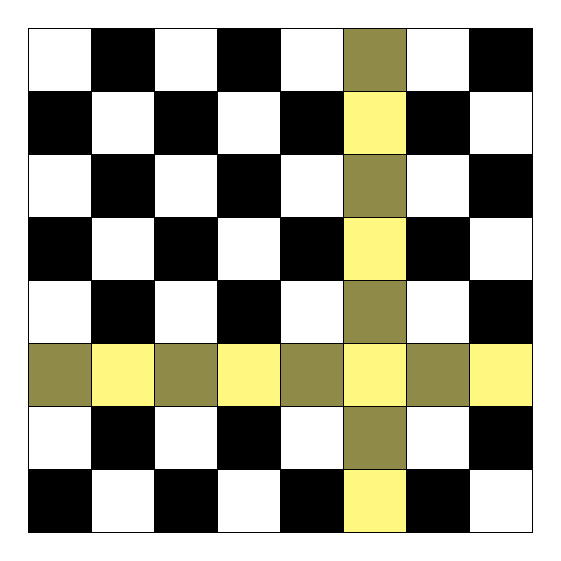
\begin{tikzpicture}
\filldraw[fill=black](-3.2,-3.2)--(-2.4000000000000004,-3.2)--(-2.4000000000000004,-2.4000000000000004)--(-3.2,-2.4000000000000004)--(-3.2,-3.2);
\filldraw[fill=white](-3.2,-2.4000000000000004)--(-2.4000000000000004,-2.4000000000000004)--(-2.4000000000000004,-1.6000000000000003)--(-3.2,-1.6000000000000003)--(-3.2,-2.4000000000000004);
\filldraw[fill=yellow!50!black](-3.2,-1.6)--(-2.4000000000000004,-1.6)--(-2.4000000000000004,-0.8)--(-3.2,-0.8)--(-3.2,-1.6);
\filldraw[fill=white](-3.2,-0.8)--(-2.4000000000000004,-0.8)--(-2.4000000000000004,0.0)--(-3.2,0.0)--(-3.2,-0.8);
\filldraw[fill=black](-3.2,0.0)--(-2.4000000000000004,0.0)--(-2.4000000000000004,0.8)--(-3.2,0.8)--(-3.2,0.0);
\filldraw[fill=white](-3.2,0.8)--(-2.4000000000000004,0.8)--(-2.4000000000000004,1.6)--(-3.2,1.6)--(-3.2,0.8);
\filldraw[fill=black](-3.2,1.6)--(-2.4000000000000004,1.6)--(-2.4000000000000004,2.4000000000000004)--(-3.2,2.4000000000000004)--(-3.2,1.6);
\filldraw[fill=white](-3.2,2.4000000000000004)--(-2.4000000000000004,2.4000000000000004)--(-2.4000000000000004,3.2)--(-3.2,3.2)--(-3.2,2.4000000000000004);
\filldraw[fill=white](-2.4000000000000004,-3.2)--(-1.6000000000000003,-3.2)--(-1.6000000000000003,-2.4000000000000004)--(-2.4000000000000004,-2.4000000000000004)--(-2.4000000000000004,-3.2);
\filldraw[fill=black](-2.4000000000000004,-2.4000000000000004)--(-1.6000000000000003,-2.4000000000000004)--(-1.6000000000000003,-1.6000000000000003)--(-2.4000000000000004,-1.6000000000000003)--(-2.4000000000000004,-2.4000000000000004);
\filldraw[fill=yellow!50!white](-2.4000000000000004,-1.6)--(-1.6000000000000003,-1.6)--(-1.6000000000000003,-0.8)--(-2.4000000000000004,-0.8)--(-2.4000000000000004,-1.6);
\filldraw[fill=black](-2.4000000000000004,-0.8)--(-1.6000000000000003,-0.8)--(-1.6000000000000003,0.0)--(-2.4000000000000004,0.0)--(-2.4000000000000004,-0.8);
\filldraw[fill=white](-2.4000000000000004,0.0)--(-1.6000000000000003,0.0)--(-1.6000000000000003,0.8)--(-2.4000000000000004,0.8)--(-2.4000000000000004,0.0);
\filldraw[fill=black](-2.4000000000000004,0.8)--(-1.6000000000000003,0.8)--(-1.6000000000000003,1.6)--(-2.4000000000000004,1.6)--(-2.4000000000000004,0.8);
\filldraw[fill=white](-2.4000000000000004,1.6)--(-1.6000000000000003,1.6)--(-1.6000000000000003,2.4000000000000004)--(-2.4000000000000004,2.4000000000000004)--(-2.4000000000000004,1.6);
\filldraw[fill=black](-2.4000000000000004,2.4000000000000004)--(-1.6000000000000003,2.4000000000000004)--(-1.6000000000000003,3.2)--(-2.4000000000000004,3.2)--(-2.4000000000000004,2.4000000000000004);
\filldraw[fill=black](-1.6,-3.2)--(-0.8,-3.2)--(-0.8,-2.4000000000000004)--(-1.6,-2.4000000000000004)--(-1.6,-3.2);
\filldraw[fill=white](-1.6,-2.4000000000000004)--(-0.8,-2.4000000000000004)--(-0.8,-1.6000000000000003)--(-1.6,-1.6000000000000003)--(-1.6,-2.4000000000000004);
\filldraw[fill=yellow!50!black](-1.6,-1.6)--(-0.8,-1.6)--(-0.8,-0.8)--(-1.6,-0.8)--(-1.6,-1.6);
\filldraw[fill=white](-1.6,-0.8)--(-0.8,-0.8)--(-0.8,0.0)--(-1.6,0.0)--(-1.6,-0.8);
\filldraw[fill=black](-1.6,0.0)--(-0.8,0.0)--(-0.8,0.8)--(-1.6,0.8)--(-1.6,0.0);
\filldraw[fill=white](-1.6,0.8)--(-0.8,0.8)--(-0.8,1.6)--(-1.6,1.6)--(-1.6,0.8);
\filldraw[fill=black](-1.6,1.6)--(-0.8,1.6)--(-0.8,2.4000000000000004)--(-1.6,2.4000000000000004)--(-1.6,1.6);
\filldraw[fill=white](-1.6,2.4000000000000004)--(-0.8,2.4000000000000004)--(-0.8,3.2)--(-1.6,3.2)--(-1.6,2.4000000000000004);
\filldraw[fill=white](-0.8,-3.2)--(0.0,-3.2)--(0.0,-2.4000000000000004)--(-0.8,-2.4000000000000004)--(-0.8,-3.2);
\filldraw[fill=black](-0.8,-2.4000000000000004)--(0.0,-2.4000000000000004)--(0.0,-1.6000000000000003)--(-0.8,-1.6000000000000003)--(-0.8,-2.4000000000000004);
\filldraw[fill=yellow!50!white](-0.8,-1.6)--(0.0,-1.6)--(0.0,-0.8)--(-0.8,-0.8)--(-0.8,-1.6);
\filldraw[fill=black](-0.8,-0.8)--(0.0,-0.8)--(0.0,0.0)--(-0.8,0.0)--(-0.8,-0.8);
\filldraw[fill=white](-0.8,0.0)--(0.0,0.0)--(0.0,0.8)--(-0.8,0.8)--(-0.8,0.0);
\filldraw[fill=black](-0.8,0.8)--(0.0,0.8)--(0.0,1.6)--(-0.8,1.6)--(-0.8,0.8);
\filldraw[fill=white](-0.8,1.6)--(0.0,1.6)--(0.0,2.4000000000000004)--(-0.8,2.4000000000000004)--(-0.8,1.6);
\filldraw[fill=black](-0.8,2.4000000000000004)--(0.0,2.4000000000000004)--(0.0,3.2)--(-0.8,3.2)--(-0.8,2.4000000000000004);
\filldraw[fill=black](0.0,-3.2)--(0.8,-3.2)--(0.8,-2.4000000000000004)--(0.0,-2.4000000000000004)--(0.0,-3.2);
\filldraw[fill=white](0.0,-2.4000000000000004)--(0.8,-2.4000000000000004)--(0.8,-1.6000000000000003)--(0.0,-1.6000000000000003)--(0.0,-2.4000000000000004);
\filldraw[fill=yellow!50!black](0.0,-1.6)--(0.8,-1.6)--(0.8,-0.8)--(0.0,-0.8)--(0.0,-1.6);
\filldraw[fill=white](0.0,-0.8)--(0.8,-0.8)--(0.8,0.0)--(0.0,0.0)--(0.0,-0.8);
\filldraw[fill=black](0.0,0.0)--(0.8,0.0)--(0.8,0.8)--(0.0,0.8)--(0.0,0.0);
\filldraw[fill=white](0.0,0.8)--(0.8,0.8)--(0.8,1.6)--(0.0,1.6)--(0.0,0.8);
\filldraw[fill=black](0.0,1.6)--(0.8,1.6)--(0.8,2.4000000000000004)--(0.0,2.4000000000000004)--(0.0,1.6);
\filldraw[fill=white](0.0,2.4000000000000004)--(0.8,2.4000000000000004)--(0.8,3.2)--(0.0,3.2)--(0.0,2.4000000000000004);
\filldraw[fill=yellow!50!white](0.8,-3.2)--(1.6,-3.2)--(1.6,-2.4000000000000004)--(0.8,-2.4000000000000004)--(0.8,-3.2);
\filldraw[fill=yellow!50!black](0.8,-2.4000000000000004)--(1.6,-2.4000000000000004)--(1.6,-1.6000000000000003)--(0.8,-1.6000000000000003)--(0.8,-2.4000000000000004);
\filldraw[fill=yellow!50!white](0.8,-1.6)--(1.6,-1.6)--(1.6,-0.8)--(0.8,-0.8)--(0.8,-1.6);
\filldraw[fill=yellow!50!black](0.8,-0.8)--(1.6,-0.8)--(1.6,0.0)--(0.8,0.0)--(0.8,-0.8);
\filldraw[fill=yellow!50!white](0.8,0.0)--(1.6,0.0)--(1.6,0.8)--(0.8,0.8)--(0.8,0.0);
\filldraw[fill=yellow!50!black](0.8,0.8)--(1.6,0.8)--(1.6,1.6)--(0.8,1.6)--(0.8,0.8);
\filldraw[fill=yellow!50!white](0.8,1.6)--(1.6,1.6)--(1.6,2.4000000000000004)--(0.8,2.4000000000000004)--(0.8,1.6);
\filldraw[fill=yellow!50!black](0.8,2.4000000000000004)--(1.6,2.4000000000000004)--(1.6,3.2)--(0.8,3.2)--(0.8,2.4000000000000004);
\filldraw[fill=black](1.6,-3.2)--(2.4000000000000004,-3.2)--(2.4000000000000004,-2.4000000000000004)--(1.6,-2.4000000000000004)--(1.6,-3.2);
\filldraw[fill=white](1.6,-2.4000000000000004)--(2.4000000000000004,-2.4000000000000004)--(2.4000000000000004,-1.6000000000000003)--(1.6,-1.6000000000000003)--(1.6,-2.4000000000000004);
\filldraw[fill=yellow!50!black](1.6,-1.6)--(2.4000000000000004,-1.6)--(2.4000000000000004,-0.8)--(1.6,-0.8)--(1.6,-1.6);
\filldraw[fill=white](1.6,-0.8)--(2.4000000000000004,-0.8)--(2.4000000000000004,0.0)--(1.6,0.0)--(1.6,-0.8);
\filldraw[fill=black](1.6,0.0)--(2.4000000000000004,0.0)--(2.4000000000000004,0.8)--(1.6,0.8)--(1.6,0.0);
\filldraw[fill=white](1.6,0.8)--(2.4000000000000004,0.8)--(2.4000000000000004,1.6)--(1.6,1.6)--(1.6,0.8);
\filldraw[fill=black](1.6,1.6)--(2.4000000000000004,1.6)--(2.4000000000000004,2.4000000000000004)--(1.6,2.4000000000000004)--(1.6,1.6);
\filldraw[fill=white](1.6,2.4000000000000004)--(2.4000000000000004,2.4000000000000004)--(2.4000000000000004,3.2)--(1.6,3.2)--(1.6,2.4000000000000004);
\filldraw[fill=white](2.4000000000000004,-3.2)--(3.2,-3.2)--(3.2,-2.4000000000000004)--(2.4000000000000004,-2.4000000000000004)--(2.4000000000000004,-3.2);
\filldraw[fill=black](2.4000000000000004,-2.4000000000000004)--(3.2,-2.4000000000000004)--(3.2,-1.6000000000000003)--(2.4000000000000004,-1.6000000000000003)--(2.4000000000000004,-2.4000000000000004);
\filldraw[fill=yellow!50!white](2.4000000000000004,-1.6)--(3.2,-1.6)--(3.2,-0.8)--(2.4000000000000004,-0.8)--(2.4000000000000004,-1.6);
\filldraw[fill=black](2.4000000000000004,-0.8)--(3.2,-0.8)--(3.2,0.0)--(2.4000000000000004,0.0)--(2.4000000000000004,-0.8);
\filldraw[fill=white](2.4000000000000004,0.0)--(3.2,0.0)--(3.2,0.8)--(2.4000000000000004,0.8)--(2.4000000000000004,0.0);
\filldraw[fill=black](2.4000000000000004,0.8)--(3.2,0.8)--(3.2,1.6)--(2.4000000000000004,1.6)--(2.4000000000000004,0.8);
\filldraw[fill=white](2.4000000000000004,1.6)--(3.2,1.6)--(3.2,2.4000000000000004)--(2.4000000000000004,2.4000000000000004)--(2.4000000000000004,1.6);
\filldraw[fill=black](2.4000000000000004,2.4000000000000004)--(3.2,2.4000000000000004)--(3.2,3.2)--(2.4000000000000004,3.2)--(2.4000000000000004,2.4000000000000004);
\end{tikzpicture}
\caption{
دو نمودار مربوط به سوال 2 قسمت الف
}
\end{figure}

\begin{figure}[h]
\centering
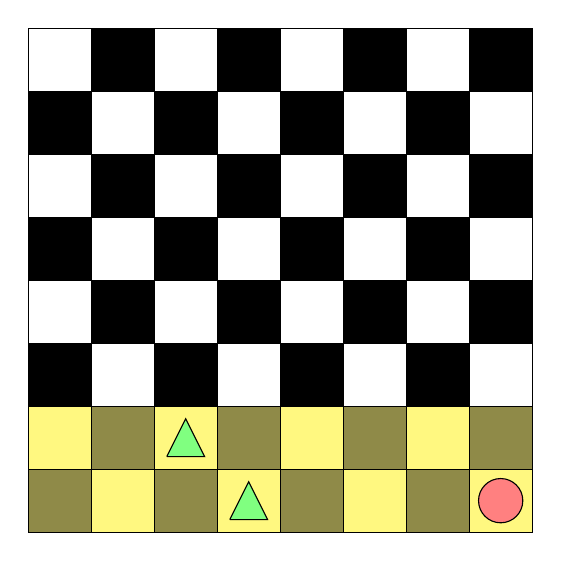
\begin{tikzpicture}
\filldraw[fill=yellow!50!black](0.8,0.8)--(1.6,0.8)--(1.6,1.6)--(0.8,1.6)--(0.8,0.8);
\filldraw[fill=yellow!50!white](0.8,1.6)--(1.6,1.6)--(1.6,2.4000000000000004)--(0.8,2.4000000000000004)--(0.8,1.6);
\filldraw[fill=black](0.8,2.4000000000000004)--(1.6,2.4000000000000004)--(1.6,3.2)--(0.8,3.2)--(0.8,2.4000000000000004);
\filldraw[fill=white](0.8,3.2)--(1.6,3.2)--(1.6,4.0)--(0.8,4.0)--(0.8,3.2);
\filldraw[fill=black](0.8,4.0)--(1.6,4.0)--(1.6,4.8)--(0.8,4.8)--(0.8,4.0);
\filldraw[fill=white](0.8,4.800000000000001)--(1.6,4.800000000000001)--(1.6,5.6000000000000005)--(0.8,5.6000000000000005)--(0.8,4.800000000000001);
\filldraw[fill=black](0.8,5.6000000000000005)--(1.6,5.6000000000000005)--(1.6,6.4)--(0.8,6.4)--(0.8,5.6000000000000005);
\filldraw[fill=white](0.8,6.4)--(1.6,6.4)--(1.6,7.2)--(0.8,7.2)--(0.8,6.4);
\filldraw[fill=yellow!50!white](1.6,0.8)--(2.4000000000000004,0.8)--(2.4000000000000004,1.6)--(1.6,1.6)--(1.6,0.8);
\filldraw[fill=yellow!50!black](1.6,1.6)--(2.4000000000000004,1.6)--(2.4000000000000004,2.4000000000000004)--(1.6,2.4000000000000004)--(1.6,1.6);
\filldraw[fill=white](1.6,2.4000000000000004)--(2.4000000000000004,2.4000000000000004)--(2.4000000000000004,3.2)--(1.6,3.2)--(1.6,2.4000000000000004);
\filldraw[fill=black](1.6,3.2)--(2.4000000000000004,3.2)--(2.4000000000000004,4.0)--(1.6,4.0)--(1.6,3.2);
\filldraw[fill=white](1.6,4.0)--(2.4000000000000004,4.0)--(2.4000000000000004,4.8)--(1.6,4.8)--(1.6,4.0);
\filldraw[fill=black](1.6,4.800000000000001)--(2.4000000000000004,4.800000000000001)--(2.4000000000000004,5.6000000000000005)--(1.6,5.6000000000000005)--(1.6,4.800000000000001);
\filldraw[fill=white](1.6,5.6000000000000005)--(2.4000000000000004,5.6000000000000005)--(2.4000000000000004,6.4)--(1.6,6.4)--(1.6,5.6000000000000005);
\filldraw[fill=black](1.6,6.4)--(2.4000000000000004,6.4)--(2.4000000000000004,7.2)--(1.6,7.2)--(1.6,6.4);
\filldraw[fill=yellow!50!black](2.4000000000000004,0.8)--(3.2,0.8)--(3.2,1.6)--(2.4000000000000004,1.6)--(2.4000000000000004,0.8);
\filldraw[fill=yellow!50!white](2.4000000000000004,1.6)--(3.2,1.6)--(3.2,2.4000000000000004)--(2.4000000000000004,2.4000000000000004)--(2.4000000000000004,1.6);
\filldraw[fill=green!50!white] (2.5600000000000005,1.7600000000000002)--(3.04,1.7600000000000002)--(2.8000000000000003,2.2399999999999998)--(2.5600000000000005,1.7600000000000002);
\filldraw[fill=black](2.4000000000000004,2.4000000000000004)--(3.2,2.4000000000000004)--(3.2,3.2)--(2.4000000000000004,3.2)--(2.4000000000000004,2.4000000000000004);
\filldraw[fill=white](2.4000000000000004,3.2)--(3.2,3.2)--(3.2,4.0)--(2.4000000000000004,4.0)--(2.4000000000000004,3.2);
\filldraw[fill=black](2.4000000000000004,4.0)--(3.2,4.0)--(3.2,4.8)--(2.4000000000000004,4.8)--(2.4000000000000004,4.0);
\filldraw[fill=white](2.4000000000000004,4.800000000000001)--(3.2,4.800000000000001)--(3.2,5.6000000000000005)--(2.4000000000000004,5.6000000000000005)--(2.4000000000000004,4.800000000000001);
\filldraw[fill=black](2.4000000000000004,5.6000000000000005)--(3.2,5.6000000000000005)--(3.2,6.4)--(2.4000000000000004,6.4)--(2.4000000000000004,5.6000000000000005);
\filldraw[fill=white](2.4000000000000004,6.4)--(3.2,6.4)--(3.2,7.2)--(2.4000000000000004,7.2)--(2.4000000000000004,6.4);
\filldraw[fill=yellow!50!white](3.2,0.8)--(4.0,0.8)--(4.0,1.6)--(3.2,1.6)--(3.2,0.8);
\filldraw[fill=green!50!white] (3.3600000000000003,0.96)--(3.84,0.96)--(3.6,1.4400000000000002)--(3.3600000000000003,0.96);
\filldraw[fill=yellow!50!black](3.2,1.6)--(4.0,1.6)--(4.0,2.4000000000000004)--(3.2,2.4000000000000004)--(3.2,1.6);
\filldraw[fill=white](3.2,2.4000000000000004)--(4.0,2.4000000000000004)--(4.0,3.2)--(3.2,3.2)--(3.2,2.4000000000000004);
\filldraw[fill=black](3.2,3.2)--(4.0,3.2)--(4.0,4.0)--(3.2,4.0)--(3.2,3.2);
\filldraw[fill=white](3.2,4.0)--(4.0,4.0)--(4.0,4.8)--(3.2,4.8)--(3.2,4.0);
\filldraw[fill=black](3.2,4.800000000000001)--(4.0,4.800000000000001)--(4.0,5.6000000000000005)--(3.2,5.6000000000000005)--(3.2,4.800000000000001);
\filldraw[fill=white](3.2,5.6000000000000005)--(4.0,5.6000000000000005)--(4.0,6.4)--(3.2,6.4)--(3.2,5.6000000000000005);
\filldraw[fill=black](3.2,6.4)--(4.0,6.4)--(4.0,7.2)--(3.2,7.2)--(3.2,6.4);
\filldraw[fill=yellow!50!black](4.0,0.8)--(4.8,0.8)--(4.8,1.6)--(4.0,1.6)--(4.0,0.8);
\filldraw[fill=yellow!50!white](4.0,1.6)--(4.8,1.6)--(4.8,2.4000000000000004)--(4.0,2.4000000000000004)--(4.0,1.6);
\filldraw[fill=black](4.0,2.4000000000000004)--(4.8,2.4000000000000004)--(4.8,3.2)--(4.0,3.2)--(4.0,2.4000000000000004);
\filldraw[fill=white](4.0,3.2)--(4.8,3.2)--(4.8,4.0)--(4.0,4.0)--(4.0,3.2);
\filldraw[fill=black](4.0,4.0)--(4.8,4.0)--(4.8,4.8)--(4.0,4.8)--(4.0,4.0);
\filldraw[fill=white](4.0,4.800000000000001)--(4.8,4.800000000000001)--(4.8,5.6000000000000005)--(4.0,5.6000000000000005)--(4.0,4.800000000000001);
\filldraw[fill=black](4.0,5.6000000000000005)--(4.8,5.6000000000000005)--(4.8,6.4)--(4.0,6.4)--(4.0,5.6000000000000005);
\filldraw[fill=white](4.0,6.4)--(4.8,6.4)--(4.8,7.2)--(4.0,7.2)--(4.0,6.4);
\filldraw[fill=yellow!50!white](4.800000000000001,0.8)--(5.6000000000000005,0.8)--(5.6000000000000005,1.6)--(4.800000000000001,1.6)--(4.800000000000001,0.8);
\filldraw[fill=yellow!50!black](4.800000000000001,1.6)--(5.6000000000000005,1.6)--(5.6000000000000005,2.4000000000000004)--(4.800000000000001,2.4000000000000004)--(4.800000000000001,1.6);
\filldraw[fill=white](4.800000000000001,2.4000000000000004)--(5.6000000000000005,2.4000000000000004)--(5.6000000000000005,3.2)--(4.800000000000001,3.2)--(4.800000000000001,2.4000000000000004);
\filldraw[fill=black](4.800000000000001,3.2)--(5.6000000000000005,3.2)--(5.6000000000000005,4.0)--(4.800000000000001,4.0)--(4.800000000000001,3.2);
\filldraw[fill=white](4.800000000000001,4.0)--(5.6000000000000005,4.0)--(5.6000000000000005,4.8)--(4.800000000000001,4.8)--(4.800000000000001,4.0);
\filldraw[fill=black](4.800000000000001,4.800000000000001)--(5.6000000000000005,4.800000000000001)--(5.6000000000000005,5.6000000000000005)--(4.800000000000001,5.6000000000000005)--(4.800000000000001,4.800000000000001);
\filldraw[fill=white](4.800000000000001,5.6000000000000005)--(5.6000000000000005,5.6000000000000005)--(5.6000000000000005,6.4)--(4.800000000000001,6.4)--(4.800000000000001,5.6000000000000005);
\filldraw[fill=black](4.800000000000001,6.4)--(5.6000000000000005,6.4)--(5.6000000000000005,7.2)--(4.800000000000001,7.2)--(4.800000000000001,6.4);
\filldraw[fill=yellow!50!black](5.6000000000000005,0.8)--(6.4,0.8)--(6.4,1.6)--(5.6000000000000005,1.6)--(5.6000000000000005,0.8);
\filldraw[fill=yellow!50!white](5.6000000000000005,1.6)--(6.4,1.6)--(6.4,2.4000000000000004)--(5.6000000000000005,2.4000000000000004)--(5.6000000000000005,1.6);
\filldraw[fill=black](5.6000000000000005,2.4000000000000004)--(6.4,2.4000000000000004)--(6.4,3.2)--(5.6000000000000005,3.2)--(5.6000000000000005,2.4000000000000004);
\filldraw[fill=white](5.6000000000000005,3.2)--(6.4,3.2)--(6.4,4.0)--(5.6000000000000005,4.0)--(5.6000000000000005,3.2);
\filldraw[fill=black](5.6000000000000005,4.0)--(6.4,4.0)--(6.4,4.8)--(5.6000000000000005,4.8)--(5.6000000000000005,4.0);
\filldraw[fill=white](5.6000000000000005,4.800000000000001)--(6.4,4.800000000000001)--(6.4,5.6000000000000005)--(5.6000000000000005,5.6000000000000005)--(5.6000000000000005,4.800000000000001);
\filldraw[fill=black](5.6000000000000005,5.6000000000000005)--(6.4,5.6000000000000005)--(6.4,6.4)--(5.6000000000000005,6.4)--(5.6000000000000005,5.6000000000000005);
\filldraw[fill=white](5.6000000000000005,6.4)--(6.4,6.4)--(6.4,7.2)--(5.6000000000000005,7.2)--(5.6000000000000005,6.4);
\filldraw[fill=yellow!50!white](6.4,0.8)--(7.2,0.8)--(7.2,1.6)--(6.4,1.6)--(6.4,0.8);
\filldraw[fill=red!50!white] (6.800000000000001,1.2000000000000002) circle (8pt);
\filldraw[fill=yellow!50!black](6.4,1.6)--(7.2,1.6)--(7.2,2.4000000000000004)--(6.4,2.4000000000000004)--(6.4,1.6);
\filldraw[fill=white](6.4,2.4000000000000004)--(7.2,2.4000000000000004)--(7.2,3.2)--(6.4,3.2)--(6.4,2.4000000000000004);
\filldraw[fill=black](6.4,3.2)--(7.2,3.2)--(7.2,4.0)--(6.4,4.0)--(6.4,3.2);
\filldraw[fill=white](6.4,4.0)--(7.2,4.0)--(7.2,4.8)--(6.4,4.8)--(6.4,4.0);
\filldraw[fill=black](6.4,4.800000000000001)--(7.2,4.800000000000001)--(7.2,5.6000000000000005)--(6.4,5.6000000000000005)--(6.4,4.800000000000001);
\filldraw[fill=white](6.4,5.6000000000000005)--(7.2,5.6000000000000005)--(7.2,6.4)--(6.4,6.4)--(6.4,5.6000000000000005);
\filldraw[fill=black](6.4,6.4)--(7.2,6.4)--(7.2,7.2)--(6.4,7.2)--(6.4,6.4);
\end{tikzpicture}
\caption{
مثالی از مات شدن شاه سفید
}
\end{figure}

\begin{figure}[h]
\centering
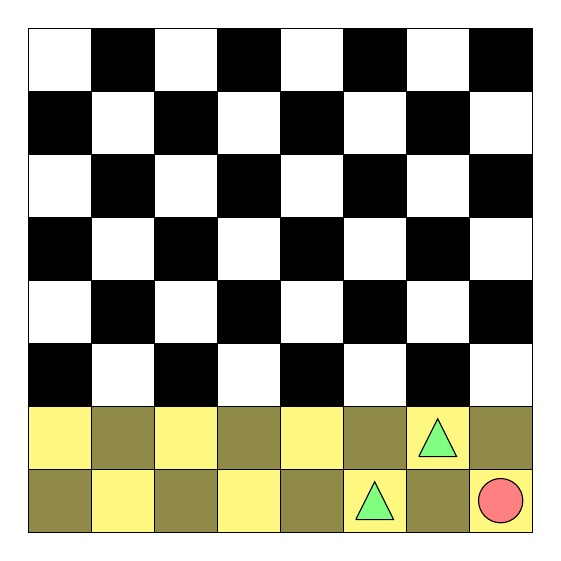
\begin{tikzpicture}
\filldraw[fill=yellow!50!black](0.8,0.8)--(1.6,0.8)--(1.6,1.6)--(0.8,1.6)--(0.8,0.8);
\filldraw[fill=yellow!50!white](0.8,1.6)--(1.6,1.6)--(1.6,2.4000000000000004)--(0.8,2.4000000000000004)--(0.8,1.6);
\filldraw[fill=black](0.8,2.4000000000000004)--(1.6,2.4000000000000004)--(1.6,3.2)--(0.8,3.2)--(0.8,2.4000000000000004);
\filldraw[fill=white](0.8,3.2)--(1.6,3.2)--(1.6,4.0)--(0.8,4.0)--(0.8,3.2);
\filldraw[fill=black](0.8,4.0)--(1.6,4.0)--(1.6,4.8)--(0.8,4.8)--(0.8,4.0);
\filldraw[fill=white](0.8,4.800000000000001)--(1.6,4.800000000000001)--(1.6,5.6000000000000005)--(0.8,5.6000000000000005)--(0.8,4.800000000000001);
\filldraw[fill=black](0.8,5.6000000000000005)--(1.6,5.6000000000000005)--(1.6,6.4)--(0.8,6.4)--(0.8,5.6000000000000005);
\filldraw[fill=white](0.8,6.4)--(1.6,6.4)--(1.6,7.2)--(0.8,7.2)--(0.8,6.4);
\filldraw[fill=yellow!50!white](1.6,0.8)--(2.4000000000000004,0.8)--(2.4000000000000004,1.6)--(1.6,1.6)--(1.6,0.8);
\filldraw[fill=yellow!50!black](1.6,1.6)--(2.4000000000000004,1.6)--(2.4000000000000004,2.4000000000000004)--(1.6,2.4000000000000004)--(1.6,1.6);
\filldraw[fill=white](1.6,2.4000000000000004)--(2.4000000000000004,2.4000000000000004)--(2.4000000000000004,3.2)--(1.6,3.2)--(1.6,2.4000000000000004);
\filldraw[fill=black](1.6,3.2)--(2.4000000000000004,3.2)--(2.4000000000000004,4.0)--(1.6,4.0)--(1.6,3.2);
\filldraw[fill=white](1.6,4.0)--(2.4000000000000004,4.0)--(2.4000000000000004,4.8)--(1.6,4.8)--(1.6,4.0);
\filldraw[fill=black](1.6,4.800000000000001)--(2.4000000000000004,4.800000000000001)--(2.4000000000000004,5.6000000000000005)--(1.6,5.6000000000000005)--(1.6,4.800000000000001);
\filldraw[fill=white](1.6,5.6000000000000005)--(2.4000000000000004,5.6000000000000005)--(2.4000000000000004,6.4)--(1.6,6.4)--(1.6,5.6000000000000005);
\filldraw[fill=black](1.6,6.4)--(2.4000000000000004,6.4)--(2.4000000000000004,7.2)--(1.6,7.2)--(1.6,6.4);
\filldraw[fill=yellow!50!black](2.4000000000000004,0.8)--(3.2,0.8)--(3.2,1.6)--(2.4000000000000004,1.6)--(2.4000000000000004,0.8);
\filldraw[fill=yellow!50!white](2.4000000000000004,1.6)--(3.2,1.6)--(3.2,2.4000000000000004)--(2.4000000000000004,2.4000000000000004)--(2.4000000000000004,1.6);
\filldraw[fill=black](2.4000000000000004,2.4000000000000004)--(3.2,2.4000000000000004)--(3.2,3.2)--(2.4000000000000004,3.2)--(2.4000000000000004,2.4000000000000004);
\filldraw[fill=white](2.4000000000000004,3.2)--(3.2,3.2)--(3.2,4.0)--(2.4000000000000004,4.0)--(2.4000000000000004,3.2);
\filldraw[fill=black](2.4000000000000004,4.0)--(3.2,4.0)--(3.2,4.8)--(2.4000000000000004,4.8)--(2.4000000000000004,4.0);
\filldraw[fill=white](2.4000000000000004,4.800000000000001)--(3.2,4.800000000000001)--(3.2,5.6000000000000005)--(2.4000000000000004,5.6000000000000005)--(2.4000000000000004,4.800000000000001);
\filldraw[fill=black](2.4000000000000004,5.6000000000000005)--(3.2,5.6000000000000005)--(3.2,6.4)--(2.4000000000000004,6.4)--(2.4000000000000004,5.6000000000000005);
\filldraw[fill=white](2.4000000000000004,6.4)--(3.2,6.4)--(3.2,7.2)--(2.4000000000000004,7.2)--(2.4000000000000004,6.4);
\filldraw[fill=yellow!50!white](3.2,0.8)--(4.0,0.8)--(4.0,1.6)--(3.2,1.6)--(3.2,0.8);
\filldraw[fill=yellow!50!black](3.2,1.6)--(4.0,1.6)--(4.0,2.4000000000000004)--(3.2,2.4000000000000004)--(3.2,1.6);
\filldraw[fill=white](3.2,2.4000000000000004)--(4.0,2.4000000000000004)--(4.0,3.2)--(3.2,3.2)--(3.2,2.4000000000000004);
\filldraw[fill=black](3.2,3.2)--(4.0,3.2)--(4.0,4.0)--(3.2,4.0)--(3.2,3.2);
\filldraw[fill=white](3.2,4.0)--(4.0,4.0)--(4.0,4.8)--(3.2,4.8)--(3.2,4.0);
\filldraw[fill=black](3.2,4.800000000000001)--(4.0,4.800000000000001)--(4.0,5.6000000000000005)--(3.2,5.6000000000000005)--(3.2,4.800000000000001);
\filldraw[fill=white](3.2,5.6000000000000005)--(4.0,5.6000000000000005)--(4.0,6.4)--(3.2,6.4)--(3.2,5.6000000000000005);
\filldraw[fill=black](3.2,6.4)--(4.0,6.4)--(4.0,7.2)--(3.2,7.2)--(3.2,6.4);
\filldraw[fill=yellow!50!black](4.0,0.8)--(4.8,0.8)--(4.8,1.6)--(4.0,1.6)--(4.0,0.8);
\filldraw[fill=yellow!50!white](4.0,1.6)--(4.8,1.6)--(4.8,2.4000000000000004)--(4.0,2.4000000000000004)--(4.0,1.6);
\filldraw[fill=black](4.0,2.4000000000000004)--(4.8,2.4000000000000004)--(4.8,3.2)--(4.0,3.2)--(4.0,2.4000000000000004);
\filldraw[fill=white](4.0,3.2)--(4.8,3.2)--(4.8,4.0)--(4.0,4.0)--(4.0,3.2);
\filldraw[fill=black](4.0,4.0)--(4.8,4.0)--(4.8,4.8)--(4.0,4.8)--(4.0,4.0);
\filldraw[fill=white](4.0,4.800000000000001)--(4.8,4.800000000000001)--(4.8,5.6000000000000005)--(4.0,5.6000000000000005)--(4.0,4.800000000000001);
\filldraw[fill=black](4.0,5.6000000000000005)--(4.8,5.6000000000000005)--(4.8,6.4)--(4.0,6.4)--(4.0,5.6000000000000005);
\filldraw[fill=white](4.0,6.4)--(4.8,6.4)--(4.8,7.2)--(4.0,7.2)--(4.0,6.4);
\filldraw[fill=yellow!50!white](4.800000000000001,0.8)--(5.6000000000000005,0.8)--(5.6000000000000005,1.6)--(4.800000000000001,1.6)--(4.800000000000001,0.8);
\filldraw[fill=green!50!white] (4.960000000000001,0.96)--(5.44,0.96)--(5.2,1.4400000000000002)--(4.960000000000001,0.96);
\filldraw[fill=yellow!50!black](4.800000000000001,1.6)--(5.6000000000000005,1.6)--(5.6000000000000005,2.4000000000000004)--(4.800000000000001,2.4000000000000004)--(4.800000000000001,1.6);
\filldraw[fill=white](4.800000000000001,2.4000000000000004)--(5.6000000000000005,2.4000000000000004)--(5.6000000000000005,3.2)--(4.800000000000001,3.2)--(4.800000000000001,2.4000000000000004);
\filldraw[fill=black](4.800000000000001,3.2)--(5.6000000000000005,3.2)--(5.6000000000000005,4.0)--(4.800000000000001,4.0)--(4.800000000000001,3.2);
\filldraw[fill=white](4.800000000000001,4.0)--(5.6000000000000005,4.0)--(5.6000000000000005,4.8)--(4.800000000000001,4.8)--(4.800000000000001,4.0);
\filldraw[fill=black](4.800000000000001,4.800000000000001)--(5.6000000000000005,4.800000000000001)--(5.6000000000000005,5.6000000000000005)--(4.800000000000001,5.6000000000000005)--(4.800000000000001,4.800000000000001);
\filldraw[fill=white](4.800000000000001,5.6000000000000005)--(5.6000000000000005,5.6000000000000005)--(5.6000000000000005,6.4)--(4.800000000000001,6.4)--(4.800000000000001,5.6000000000000005);
\filldraw[fill=black](4.800000000000001,6.4)--(5.6000000000000005,6.4)--(5.6000000000000005,7.2)--(4.800000000000001,7.2)--(4.800000000000001,6.4);
\filldraw[fill=yellow!50!black](5.6000000000000005,0.8)--(6.4,0.8)--(6.4,1.6)--(5.6000000000000005,1.6)--(5.6000000000000005,0.8);
\filldraw[fill=yellow!50!white](5.6000000000000005,1.6)--(6.4,1.6)--(6.4,2.4000000000000004)--(5.6000000000000005,2.4000000000000004)--(5.6000000000000005,1.6);
\filldraw[fill=green!50!white] (5.760000000000001,1.7600000000000002)--(6.24,1.7600000000000002)--(6.0,2.2399999999999998)--(5.760000000000001,1.7600000000000002);
\filldraw[fill=black](5.6000000000000005,2.4000000000000004)--(6.4,2.4000000000000004)--(6.4,3.2)--(5.6000000000000005,3.2)--(5.6000000000000005,2.4000000000000004);
\filldraw[fill=white](5.6000000000000005,3.2)--(6.4,3.2)--(6.4,4.0)--(5.6000000000000005,4.0)--(5.6000000000000005,3.2);
\filldraw[fill=black](5.6000000000000005,4.0)--(6.4,4.0)--(6.4,4.8)--(5.6000000000000005,4.8)--(5.6000000000000005,4.0);
\filldraw[fill=white](5.6000000000000005,4.800000000000001)--(6.4,4.800000000000001)--(6.4,5.6000000000000005)--(5.6000000000000005,5.6000000000000005)--(5.6000000000000005,4.800000000000001);
\filldraw[fill=black](5.6000000000000005,5.6000000000000005)--(6.4,5.6000000000000005)--(6.4,6.4)--(5.6000000000000005,6.4)--(5.6000000000000005,5.6000000000000005);
\filldraw[fill=white](5.6000000000000005,6.4)--(6.4,6.4)--(6.4,7.2)--(5.6000000000000005,7.2)--(5.6000000000000005,6.4);
\filldraw[fill=yellow!50!white](6.4,0.8)--(7.2,0.8)--(7.2,1.6)--(6.4,1.6)--(6.4,0.8);
\filldraw[fill=red!50!white] (6.800000000000001,1.2000000000000002) circle (8pt);
\filldraw[fill=yellow!50!black](6.4,1.6)--(7.2,1.6)--(7.2,2.4000000000000004)--(6.4,2.4000000000000004)--(6.4,1.6);
\filldraw[fill=white](6.4,2.4000000000000004)--(7.2,2.4000000000000004)--(7.2,3.2)--(6.4,3.2)--(6.4,2.4000000000000004);
\filldraw[fill=black](6.4,3.2)--(7.2,3.2)--(7.2,4.0)--(6.4,4.0)--(6.4,3.2);
\filldraw[fill=white](6.4,4.0)--(7.2,4.0)--(7.2,4.8)--(6.4,4.8)--(6.4,4.0);
\filldraw[fill=black](6.4,4.800000000000001)--(7.2,4.800000000000001)--(7.2,5.6000000000000005)--(6.4,5.6000000000000005)--(6.4,4.800000000000001);
\filldraw[fill=white](6.4,5.6000000000000005)--(7.2,5.6000000000000005)--(7.2,6.4)--(6.4,6.4)--(6.4,5.6000000000000005);
\filldraw[fill=black](6.4,6.4)--(7.2,6.4)--(7.2,7.2)--(6.4,7.2)--(6.4,6.4);
\end{tikzpicture}
\vspace{10mm}
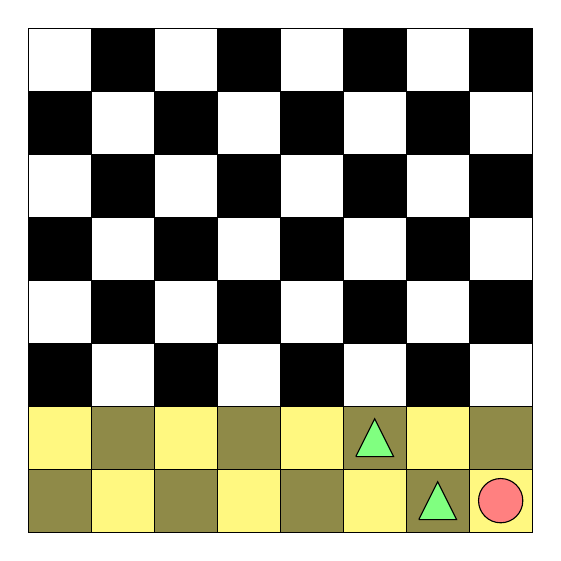
\begin{tikzpicture}
\filldraw[fill=yellow!50!black](0.8,0.8)--(1.6,0.8)--(1.6,1.6)--(0.8,1.6)--(0.8,0.8);
\filldraw[fill=yellow!50!white](0.8,1.6)--(1.6,1.6)--(1.6,2.4000000000000004)--(0.8,2.4000000000000004)--(0.8,1.6);
\filldraw[fill=black](0.8,2.4000000000000004)--(1.6,2.4000000000000004)--(1.6,3.2)--(0.8,3.2)--(0.8,2.4000000000000004);
\filldraw[fill=white](0.8,3.2)--(1.6,3.2)--(1.6,4.0)--(0.8,4.0)--(0.8,3.2);
\filldraw[fill=black](0.8,4.0)--(1.6,4.0)--(1.6,4.8)--(0.8,4.8)--(0.8,4.0);
\filldraw[fill=white](0.8,4.800000000000001)--(1.6,4.800000000000001)--(1.6,5.6000000000000005)--(0.8,5.6000000000000005)--(0.8,4.800000000000001);
\filldraw[fill=black](0.8,5.6000000000000005)--(1.6,5.6000000000000005)--(1.6,6.4)--(0.8,6.4)--(0.8,5.6000000000000005);
\filldraw[fill=white](0.8,6.4)--(1.6,6.4)--(1.6,7.2)--(0.8,7.2)--(0.8,6.4);
\filldraw[fill=yellow!50!white](1.6,0.8)--(2.4000000000000004,0.8)--(2.4000000000000004,1.6)--(1.6,1.6)--(1.6,0.8);
\filldraw[fill=yellow!50!black](1.6,1.6)--(2.4000000000000004,1.6)--(2.4000000000000004,2.4000000000000004)--(1.6,2.4000000000000004)--(1.6,1.6);
\filldraw[fill=white](1.6,2.4000000000000004)--(2.4000000000000004,2.4000000000000004)--(2.4000000000000004,3.2)--(1.6,3.2)--(1.6,2.4000000000000004);
\filldraw[fill=black](1.6,3.2)--(2.4000000000000004,3.2)--(2.4000000000000004,4.0)--(1.6,4.0)--(1.6,3.2);
\filldraw[fill=white](1.6,4.0)--(2.4000000000000004,4.0)--(2.4000000000000004,4.8)--(1.6,4.8)--(1.6,4.0);
\filldraw[fill=black](1.6,4.800000000000001)--(2.4000000000000004,4.800000000000001)--(2.4000000000000004,5.6000000000000005)--(1.6,5.6000000000000005)--(1.6,4.800000000000001);
\filldraw[fill=white](1.6,5.6000000000000005)--(2.4000000000000004,5.6000000000000005)--(2.4000000000000004,6.4)--(1.6,6.4)--(1.6,5.6000000000000005);
\filldraw[fill=black](1.6,6.4)--(2.4000000000000004,6.4)--(2.4000000000000004,7.2)--(1.6,7.2)--(1.6,6.4);
\filldraw[fill=yellow!50!black](2.4000000000000004,0.8)--(3.2,0.8)--(3.2,1.6)--(2.4000000000000004,1.6)--(2.4000000000000004,0.8);
\filldraw[fill=yellow!50!white](2.4000000000000004,1.6)--(3.2,1.6)--(3.2,2.4000000000000004)--(2.4000000000000004,2.4000000000000004)--(2.4000000000000004,1.6);
\filldraw[fill=black](2.4000000000000004,2.4000000000000004)--(3.2,2.4000000000000004)--(3.2,3.2)--(2.4000000000000004,3.2)--(2.4000000000000004,2.4000000000000004);
\filldraw[fill=white](2.4000000000000004,3.2)--(3.2,3.2)--(3.2,4.0)--(2.4000000000000004,4.0)--(2.4000000000000004,3.2);
\filldraw[fill=black](2.4000000000000004,4.0)--(3.2,4.0)--(3.2,4.8)--(2.4000000000000004,4.8)--(2.4000000000000004,4.0);
\filldraw[fill=white](2.4000000000000004,4.800000000000001)--(3.2,4.800000000000001)--(3.2,5.6000000000000005)--(2.4000000000000004,5.6000000000000005)--(2.4000000000000004,4.800000000000001);
\filldraw[fill=black](2.4000000000000004,5.6000000000000005)--(3.2,5.6000000000000005)--(3.2,6.4)--(2.4000000000000004,6.4)--(2.4000000000000004,5.6000000000000005);
\filldraw[fill=white](2.4000000000000004,6.4)--(3.2,6.4)--(3.2,7.2)--(2.4000000000000004,7.2)--(2.4000000000000004,6.4);
\filldraw[fill=yellow!50!white](3.2,0.8)--(4.0,0.8)--(4.0,1.6)--(3.2,1.6)--(3.2,0.8);
\filldraw[fill=yellow!50!black](3.2,1.6)--(4.0,1.6)--(4.0,2.4000000000000004)--(3.2,2.4000000000000004)--(3.2,1.6);
\filldraw[fill=white](3.2,2.4000000000000004)--(4.0,2.4000000000000004)--(4.0,3.2)--(3.2,3.2)--(3.2,2.4000000000000004);
\filldraw[fill=black](3.2,3.2)--(4.0,3.2)--(4.0,4.0)--(3.2,4.0)--(3.2,3.2);
\filldraw[fill=white](3.2,4.0)--(4.0,4.0)--(4.0,4.8)--(3.2,4.8)--(3.2,4.0);
\filldraw[fill=black](3.2,4.800000000000001)--(4.0,4.800000000000001)--(4.0,5.6000000000000005)--(3.2,5.6000000000000005)--(3.2,4.800000000000001);
\filldraw[fill=white](3.2,5.6000000000000005)--(4.0,5.6000000000000005)--(4.0,6.4)--(3.2,6.4)--(3.2,5.6000000000000005);
\filldraw[fill=black](3.2,6.4)--(4.0,6.4)--(4.0,7.2)--(3.2,7.2)--(3.2,6.4);
\filldraw[fill=yellow!50!black](4.0,0.8)--(4.8,0.8)--(4.8,1.6)--(4.0,1.6)--(4.0,0.8);
\filldraw[fill=yellow!50!white](4.0,1.6)--(4.8,1.6)--(4.8,2.4000000000000004)--(4.0,2.4000000000000004)--(4.0,1.6);
\filldraw[fill=black](4.0,2.4000000000000004)--(4.8,2.4000000000000004)--(4.8,3.2)--(4.0,3.2)--(4.0,2.4000000000000004);
\filldraw[fill=white](4.0,3.2)--(4.8,3.2)--(4.8,4.0)--(4.0,4.0)--(4.0,3.2);
\filldraw[fill=black](4.0,4.0)--(4.8,4.0)--(4.8,4.8)--(4.0,4.8)--(4.0,4.0);
\filldraw[fill=white](4.0,4.800000000000001)--(4.8,4.800000000000001)--(4.8,5.6000000000000005)--(4.0,5.6000000000000005)--(4.0,4.800000000000001);
\filldraw[fill=black](4.0,5.6000000000000005)--(4.8,5.6000000000000005)--(4.8,6.4)--(4.0,6.4)--(4.0,5.6000000000000005);
\filldraw[fill=white](4.0,6.4)--(4.8,6.4)--(4.8,7.2)--(4.0,7.2)--(4.0,6.4);
\filldraw[fill=yellow!50!white](4.800000000000001,0.8)--(5.6000000000000005,0.8)--(5.6000000000000005,1.6)--(4.800000000000001,1.6)--(4.800000000000001,0.8);
\filldraw[fill=yellow!50!black](4.800000000000001,1.6)--(5.6000000000000005,1.6)--(5.6000000000000005,2.4000000000000004)--(4.800000000000001,2.4000000000000004)--(4.800000000000001,1.6);
\filldraw[fill=green!50!white] (4.960000000000001,1.7600000000000002)--(5.44,1.7600000000000002)--(5.2,2.2399999999999998)--(4.960000000000001,1.7600000000000002);
\filldraw[fill=white](4.800000000000001,2.4000000000000004)--(5.6000000000000005,2.4000000000000004)--(5.6000000000000005,3.2)--(4.800000000000001,3.2)--(4.800000000000001,2.4000000000000004);
\filldraw[fill=black](4.800000000000001,3.2)--(5.6000000000000005,3.2)--(5.6000000000000005,4.0)--(4.800000000000001,4.0)--(4.800000000000001,3.2);
\filldraw[fill=white](4.800000000000001,4.0)--(5.6000000000000005,4.0)--(5.6000000000000005,4.8)--(4.800000000000001,4.8)--(4.800000000000001,4.0);
\filldraw[fill=black](4.800000000000001,4.800000000000001)--(5.6000000000000005,4.800000000000001)--(5.6000000000000005,5.6000000000000005)--(4.800000000000001,5.6000000000000005)--(4.800000000000001,4.800000000000001);
\filldraw[fill=white](4.800000000000001,5.6000000000000005)--(5.6000000000000005,5.6000000000000005)--(5.6000000000000005,6.4)--(4.800000000000001,6.4)--(4.800000000000001,5.6000000000000005);
\filldraw[fill=black](4.800000000000001,6.4)--(5.6000000000000005,6.4)--(5.6000000000000005,7.2)--(4.800000000000001,7.2)--(4.800000000000001,6.4);
\filldraw[fill=yellow!50!black](5.6000000000000005,0.8)--(6.4,0.8)--(6.4,1.6)--(5.6000000000000005,1.6)--(5.6000000000000005,0.8);
\filldraw[fill=green!50!white] (5.760000000000001,0.96)--(6.24,0.96)--(6.0,1.4400000000000002)--(5.760000000000001,0.96);
\filldraw[fill=yellow!50!white](5.6000000000000005,1.6)--(6.4,1.6)--(6.4,2.4000000000000004)--(5.6000000000000005,2.4000000000000004)--(5.6000000000000005,1.6);
\filldraw[fill=black](5.6000000000000005,2.4000000000000004)--(6.4,2.4000000000000004)--(6.4,3.2)--(5.6000000000000005,3.2)--(5.6000000000000005,2.4000000000000004);
\filldraw[fill=white](5.6000000000000005,3.2)--(6.4,3.2)--(6.4,4.0)--(5.6000000000000005,4.0)--(5.6000000000000005,3.2);
\filldraw[fill=black](5.6000000000000005,4.0)--(6.4,4.0)--(6.4,4.8)--(5.6000000000000005,4.8)--(5.6000000000000005,4.0);
\filldraw[fill=white](5.6000000000000005,4.800000000000001)--(6.4,4.800000000000001)--(6.4,5.6000000000000005)--(5.6000000000000005,5.6000000000000005)--(5.6000000000000005,4.800000000000001);
\filldraw[fill=black](5.6000000000000005,5.6000000000000005)--(6.4,5.6000000000000005)--(6.4,6.4)--(5.6000000000000005,6.4)--(5.6000000000000005,5.6000000000000005);
\filldraw[fill=white](5.6000000000000005,6.4)--(6.4,6.4)--(6.4,7.2)--(5.6000000000000005,7.2)--(5.6000000000000005,6.4);
\filldraw[fill=yellow!50!white](6.4,0.8)--(7.2,0.8)--(7.2,1.6)--(6.4,1.6)--(6.4,0.8);
\filldraw[fill=red!50!white] (6.800000000000001,1.2000000000000002) circle (8pt);
\filldraw[fill=yellow!50!black](6.4,1.6)--(7.2,1.6)--(7.2,2.4000000000000004)--(6.4,2.4000000000000004)--(6.4,1.6);
\filldraw[fill=white](6.4,2.4000000000000004)--(7.2,2.4000000000000004)--(7.2,3.2)--(6.4,3.2)--(6.4,2.4000000000000004);
\filldraw[fill=black](6.4,3.2)--(7.2,3.2)--(7.2,4.0)--(6.4,4.0)--(6.4,3.2);
\filldraw[fill=white](6.4,4.0)--(7.2,4.0)--(7.2,4.8)--(6.4,4.8)--(6.4,4.0);
\filldraw[fill=black](6.4,4.800000000000001)--(7.2,4.800000000000001)--(7.2,5.6000000000000005)--(6.4,5.6000000000000005)--(6.4,4.800000000000001);
\filldraw[fill=white](6.4,5.6000000000000005)--(7.2,5.6000000000000005)--(7.2,6.4)--(6.4,6.4)--(6.4,5.6000000000000005);
\filldraw[fill=black](6.4,6.4)--(7.2,6.4)--(7.2,7.2)--(6.4,7.2)--(6.4,6.4);
\end{tikzpicture}
\caption{
حالت هایی که به مات شدن منجر نمی شوند.
}
\end{figure}

\newpage

\QA

هر مجموعه‌ی $n$ عضوی، 
$
2^n
$
زیرمجموعه دارد. ابتدا یکی از زیرمجموعه‌های 
$
k
$
عضوی را به تصادف بر می‌داریم. این کار به 
$
\binom{n}{k}
$
طریق امکان دارد. برای آن که زیرمجموعه‌ی دیگر، با زیرمجموعه‌ی انتخاب شده ناسازگار باشد، باید اعضای آن از بین 
$
n-k
$
عضو باقیمانده به 
$
2^{n-k}
$
طریق ممکن انتخاب شوند. در نتیجه تعداد حالات مطلوب (برای هر زیرمجموعه با هر تعداد عضو)، طبق اصل ضرب برابر
$
\sum_{k=0}^n\binom{n}{k}2^{n-k}
$
خواهد بود. با این حال، باید دقت شود که تعدادی از حالات تکراری اند. به طور مثال، امکان دارد زیرمجموعه‌ی 
$
\{1,3,n\}
$
، در دفعه‌ی اول و زیرمجموعه‌ی 
$
\{2,4,n-1\}
$
در دفعه‌ی دوم از بین اعضای باقیمانده انتخاب شود؛ یا بالعکس. همچنین، حالتی که هر دو زیرمجموعه تهی باشند، شمرده شده است که با وجود ناسازگاری، متمایز نیستند. پس باید از تعداد کل حالات مطلوب کنار گذاشته شوند. در نتیجه، حالات مطلوب برداشتن دو زیرمجموعه‌ی ناسازگار متمایز، برابر
$
\frac{
[\sum_{k=0}^n\binom{n}{k}2^{n-k}]-1
}{2}
$
و احتمال مطلوب، برابر
$
\frac{
\frac{
[\sum_{k=0}^n\binom{n}{k}2^{n-k}]-1
}{2}
}{
\binom{2^n}{2}
}
$
خواهد بود.

(با ساده سازی، می توان احتمال را به صورت زیر نیز نوشت
$$
\frac{
3^n-1
}{
2^n(2^n-1)
}
$$
)

\QA

از آنجا که هر رخداد سکه (پشت یا رو) معادل با پرتاب یک یا دو تاس است، پیشامد های زیر را تعریف می‌کنیم:
\eqn{
&
A=\text{
پیشامد رو آمدن سکه (پرتاب 1 تاس)
}
\\&
B=\text{
پیشامد پشت آمدن سکه (پرتاب 2 تاس)
}
\\&
C_n=\text{
پیشامد رو آمدن عدد $n$
}
}{}
می‌دانیم
$$
P(A)=P(B)=0.5.
$$
از طرفی
\eqn{
&
P(C_n|A)=\begin{cases}
\frac{1}{6}&,\quad n=1,2,\cdots,6\\
0&,\quad n=7,8,\cdots,12
\end{cases}
}{}
و
\eqn{
&
P(C_n|B)=\begin{cases}
0&,\quad n=1\\
\frac{6-|n-7|}{36}&,\quad n=2,\cdots,12
\end{cases}
}{}
مطلوبست $P(C_n)$. در نتیجه طبق قاعده‌ی احتمال کل
\eqn{
P(C_n)&=P(A)P(C_n|A)+P(B)P(C_n|B)
\\&=\frac{1}{2}P(C_n|A)+\frac{1}{2}P(C_n|B)
\\&=
\begin{cases}
\frac{1}{12}&,\quad n=1,2,\cdots,6\\
0&,\quad n=7,8,\cdots,12
\end{cases}
\\&+
\begin{cases}
0&,\quad n=1\\
\frac{6-|n-7|}{72}&,\quad n=2,\cdots,12
\end{cases}
}{}

با ساده سازی خواهیم داشت
$$
P(C_n)=
\begin{cases}
\frac{1}{12}&,\quad n=1\\
\frac{5+n}{72}&,\quad n=2,\cdots,6\\
\frac{13-n}{72}&,\quad n=7,\cdots,12
\end{cases}
$$
\QA

راه اول)

پیشامدهای زیر را تعریف می‌کنیم:
\eqn{
&
A_n=\text{
پیشامد سیاه بودن $n$ توپ از 3 توپ بیرون آمده در بار اول
}
\\&
B=\text{
پیشامد سفید بودن توپ انتخابی از 3 توپ بیرون آمده در بار اول
}
}{}
در نتیجه
\eqn{
P(A_n)=\frac{\binom{10}{3-n}\binom{7}{n}}{\binom{17}{3}}
}{}
همچنین
\eqn{
P(B|A_n)=\frac{3-n}{3}
}{}

مطلوبست
$
P(B|A_1\cup A_2\cup A_3)
$.
در نتیجه
\eqn{
&
P(B|A_1\cup A_2\cup A_3)
=
\frac{
P(B\cap[A_1\cup A_2\cup A_3])
}{
P(A_1\cup A_2\cup A_3)
}
\\&=
\frac{
P(B\cap A_1)+P(B\cap A_2)+P(B\cap A_3)
}{
P(A_1)+P(A_2)+P(A_3)
}
\\&=
\frac{
P(B|A_1)P(A_1)+P(B|A_2)P(A_2)+P(B|A_3)P(A_3)
}{
1-P(A_0)
}
\\&=
\frac{
\frac{2}{3}\times \frac{\binom{10}{2}\binom{7}{1}}{\binom{17}{3}}+
\frac{1}{3}\times \frac{\binom{10}{1}\binom{7}{2}}{\binom{17}{3}}+0\times P(A_3)
}{
1-\frac{\binom{10}{3}}{\binom{17}{3}}
}
\\&=\frac{1}{2}
}{}

راه دوم)

پیشامدهای زیر را تعریف می‌کنیم:
\eqn{
&
A=\text{
پیشامد سیاه بودن دست کم یک توپ از 3 توپ بیرون آمده در بار اول
}
\\&
B=\text{
پیشامد سفید بودن توپ انتخابی از 3 توپ بیرون آمده در بار اول
}
}{}

در نتیجه
\eqn{
&P(A)=1-P(A')=P(\text{
پیشامد سیاه بودن هیچ توپ از 3 توپ بیرون آمده در بار اول
})
\\&=
P(\text{
پیشامد سفید بودن هر سه توپ بیرون آمده در بار اول
})
\\&=
1-\frac{\binom{10}{3}}{\binom{17}{3}}
\\&=
1-\frac{10\times 9\times 8}{17\times 16\times 15}
\\&=
\frac{14}{17}
}{}
مطلوبست
$
P(B|A)
$
. در نتیجه
\eqn{
P(B|A)&=\frac{P(B\cap A)}{P(A)}
\\&=\frac{P(B\cap A)+P(B\cap A')-P(B\cap A')}{P(A)}
\\&=\frac{P(B)-P(B|A')P(A')}{P(A)}
\\&=\frac{P(B)-P(A')}{P(A)}
}{}
از طرفی، پیشامد $B$ معادل با این است که توپی از کیسه برداریم و سفید باشد (به عبارت دیگر، از 3 توپ برداشته شده‌ی مرحله‌ی قبل، به طور مثال با بستن چشم بی خبر باشیم). در نتیجه
$$
P(B)=\frac{10}{17}
$$
و با جایگذاری خواهیم داشت
\eqn{
P(B|A)=\frac{P(B)-P(A')}{P(A)}
=\frac{\frac{10}{17}-\frac{3}{17}}{\frac{14}{17}}=\frac{1}{2}.
}{}















\QA

پیشامدهای زیر را تعریف می‌کنیم:
\eqn{
&
A=\text{
پیشامد انتخاب کیسه‌ی 1
}
\\&
B=\text{
پیشامد انتخاب کیسه‌ی 2
}
\\&
C=\text{
پیشامد سفید نبودن توپ انتخابی
}
}{}
در نتیجه خواهیم داشت
\eqn{
P(A)=P(B)=0.5
}{}
و
\eqn{
P(C|A)=\frac{7}{17}\quad,\quad P(C|B)=\frac{7}{9}
}{}
مطلوب است 
$P(B|C)$
. در نتیجه طبق قاعده‌ی احتمال بیز
\eqn{
P(B|C)&=\frac{P(C|B)P(B)}{P(C|A)P(A)+P(C|B)P(B)}
\\&=
\frac{
\frac{7}{9}\times \frac{1}{2}
}{
\frac{7}{9}\times \frac{1}{2}
+
\frac{7}{17}\times \frac{1}{2}
}=\frac{17}{26}
}{}

مکمل پیشامد مطلوب آن است که خانواده، دارای هیچ فرزند پسر یا هیچ فرزند دختری نباشد. احتمال پیشامد اخیر برابر است با
$$
(\frac{1}{2})^n+(\frac{1}{2})^n=(\frac{1}{2})^{n-1}؛
$$
در نتیجه، احتمال مطلوب برابر است با
$$
1-(\frac{1}{2})^{n-1}
$$
که باید بیشتر از یا مساوی با $0.95$ باشد. در نتیجه
\eqn{
&1-(\frac{1}{2})^{n-1}\ge 0.95
\\&\implies
(\frac{1}{2})^{n-1}\le 0.05
\\&\implies
2^{n-1}\ge 20
\\&\implies
n-1\ge \log_220
\\&\implies
n\ge 6
}{}



\chapter{آزمایش های تکراری}

\QA

الف) پیشامد مطلوب، عبارتست از آنکه دقیقا 2 بار عدد زوج یا دقیقا 3 بار عدد زوج بیاید. احتمال عدد زوج آمدن برابر $0.5$ است. در نتیجه احتمال مطلوب برابر است با
$$
\binom{3}{2}(\frac{1}{2})^3+\binom{3}{3}(\frac{1}{2})^3=\frac{1}{2}.
$$

ب) مجموع اعداد رو آمده در این 3 پرتاب، در حالات زیر برابر 5 می شود:

- دو بار 1 و یکبار 3 بیاید.

- دوبار 2 و یکبار 1 بیاید.

هر یک از حالات فوق، دارای احتمال
$$
\binom{3}{1}(\frac{1}{6})^3=\frac{1}{72}
$$
هستند؛ در نتیجه احتمال مطلوب، برابر 
$
\frac{1}{72}+\frac{1}{72}=\frac{1}{36}
$
خواهد بود.

پ) برای رو آمدن مضرب 3، باید اعداد 3 و 6 ظاهر شوند. احتمال این موضوع برابر 
$
\frac{1}{3}
$
است و چون نتیجه‌ی سایر پرتاب ها مهم نیست، احتمال مطلوب نیز 
$
\frac{1}{3}
$
خواهد بود.

سوال 5) الف) این حالت زمانی ممکن است که تیم $A$ پس از 6 دست، در حداقل 5 دست پیروز شده باشد که این احتمال برابر با احتمال پیروزی در دقیقا 5 دست یا دقیقا 6 دست از 6 دست اول است؛ بنابراین
$$
p=\binom{6}{5}p^5(1-p)+\binom{6}{6}p^6=p^5(6-5p)
$$
ب) 
\eqn{
&\Pr\{
\text{\rl{باخت در حداقل یک دست به تیم $B$}}|\text{\rl{برد تیم $A$}}
\}
\\&=
{
\Pr\{
\text{\rl{باخت در حداقل یک دست به تیم $B$}}\cap\text{\rl{برد تیم $A$}}
\}
\over
\Pr\{
\text{\rl{برد تیم $A$}}
\}
}
}{}
احتمال آن که تیم \lr{A} بازی را ببرد و هیچ دستی را به تیم \lr{B} نبازد برابر $p^9$ است. هم چنین احتمال برد تیم $A$ نیز برابر 
$
\sum_{k=5}^{9}\binom{9}{k}p^k(1-p)^{9-k}
$
 خواهد بود. در نتیجه احتمال مطلوب به شکل زیر محاسبه می‌شود:
$$
1-{p^9\over \sum_{k=5}^{9}\binom{9}{k}p^k(1-p)^{9-k}}
$$
ج) تیم $A$ در صورتی بازی را می برد که حداقل 4 دست از 8 دست باقی مانده را ببرد. این احتمال برابرست با:
$$
{\sum_{k=4}^{8}\binom{8}{k}\over 2^8}\approx 0.6367
$$

سوال 5)

الف) در رشته متوالی لامپ ها، لامپ ها به صورت پشت سر هم به یکدیگر وصل شده اند؛ پس رشته زمانی روشن است که تمام لامپ ها سالم باشند. احتمال این امر برابر 
$
(1-p)^n
$
است.

ب) در رشته‌ی موازی لامپ ها، یکی از سرهای همه‌ی لامپ ها به یک نقطه و سر دیگر تمام لامپ ها به نقطه‌ی دیگر وصل شده اند؛ پس رشته زمانی خراب می شود که همه ی لامپ های آن خراب باشند. بنابراین احتمال روشن شدن رشته برابر 
$
1-p^n
$
است.

\QA

سوال 1) قضیه‌ی دوموآو - لاپلاس اذعان می کند:
\eqn{
\binom{n}{k}p^k(1-p)^{n-k}\approx
{1\over \sqrt{2\pi np(1-p)}}e^{-{(k-np)^2\over 2np(1-p)}}
}{}
هنگامی که $k$ نزدیک به $np$ باشد. در اینجا می خواهیم شهودی از میزان این نزدیکی پیدا کنیم. به ازای $k$ های مختلف داریم:
$$
\begin{cases}
k=1&,\quad \text{\rl{خطای نسبی}}\sim 10^{80}
\\
k=300&,\quad \text{\rl{خطای نسبی}}\approx 7.99
\\
k=490&,\quad \text{\rl{خطای نسبی}}\approx 6.34\times 10^{-5}
\end{cases}
$$
شایان گفتن است که در دو حالت اول، مقدارهای دقیق و تقریبی احتمال تقریبا برابر صفر هستند.

سوال 1) الف) به دلیل استقلال پرتاب ها، می توان تنها دو پرتاب اول و آخر را در نظر گرفت. بنابراین احتمال اینکه در هر دو پرتاب سکه رو یا پشت بیاید برابر $0.5$ است.

ب)
\eqn{
\{
\text{
پیشامد حداقل 2 رو و 3 پشت
}\}
&=
\{
\text{
پیشامد 2 رو و 5 پشت
}\}
\\&\cup
\{
\text{
پیشامد 3 رو و 4 پشت
}\}
\\&\cup
\{
\text{
پیشامد 4 رو و 3 پشت
}\}
\\&=
\binom{7}{2}\left({1\over 2}\right)^7
+\binom{7}{3}\left({1\over 2}\right)^7
+\binom{7}{4}\left({1\over 2}\right)^7
\\&={91\over 128}\approx 0.71
}{}

پ) تعریف می کنیم:
\eqn{
&
A=
\text{
پیشامد رو آمدن در سه پرتاب اول
}
\\&
B=
\text{
پیشامد پشت آمدن در سه پرتاب اول
}
\\&
C=\text{
دقیقا 4 بار رو آمدن سکه در 7 پرتاب
}
}{}
با تعاریف فوق مطلوب است:
$$
\Pr(
C|A\cup B
)
$$
بنابراین
\eqn{
\Pr(
C|A\cup B
)
&={p(C\cap[A\cup B])\over p(A\cup B)}
\\&={p(C\cap A)+p(C\cap B)\over p(A)+p(B)}
\\&={p(C|A)p(A)+\left({1\over 2}\right)^7\over {1\over 8}+{1\over 8}}
\\&={\binom{4}{1}\left({1\over 2}\right)^4\cdot{1\over 8}+\left({1\over 2}\right)^7\over {1\over 4}}
\\&={5\over 32}\approx 0.16
}{}

سوال 2) الف) پیشامد مطلوب برابر است با:
\eqn{
\text{
پیشامد جمع 7
}
&=
\text{
یک بار رو آمدن عدد 3 و چهار بار رو آمدن عدد 1
}
\\&\cup
\text{
دو بار رو آمدن عدد 2 و سه بار رو آمدن عدد 1
}
\\&=
\binom{5}{1}\left({1\over 6}\right)^1\left({1\over 6}\right)^4
\\&+
\binom{5}{2}\left({1\over 6}\right)^2\left({1\over 6}\right)^3
\\&={5\over 2592}\approx 0.002
}{}

ب) 
\eqn{
\text{
پیشامد مطلوب
}
&=
\text{
رو آمدن 4 در پرتاب آخر و 1 در چهار پرتاب اول
}
\\&\cup
\text{
رو آمدن 5 در پرتاب آخر، سه تا 1 و یک 2 در چهار پرتاب اول
}
\\&\cup
\text{
رو آمدن 6 در پرتاب آخر و سه تا 1 و یک 3 در چهار پرتاب اول
}
\\&\cup
\text{
رو آمدن 6 در پرتاب آخر و دو تا 2 و دو تا 1 در چهار پرتاب اول
}
\\&=
\left({1\over 6}\right)^5
+
\binom{4}{3}\left({1\over 6}\right)^4\times {1\over 6}
+
\binom{4}{3}\left({1\over 6}\right)^4\times {1\over 6}
+
\binom{4}{2}\left({1\over 6}\right)^4\times {1\over 6}
\\&={5\over 2592}\approx 0.002
}{}

سوال 3) الف) این اتفاق تنها زمان می افتد که حداکثر 8 ماشین وارد بزرگراه شوند. مکمل این پیشامد حالتی است که هر 9 ماشین همزمان وارد بزرگراه شوند که این رخداد دارای احتمال 
$
p^9
$
است. پس احتمال مطلوب، 
$
1-p^9
$
خواهد بود.

ب) $p$ چقدر باشد تا احتمال قسمت الف بیشتر از $0.99$ باشد؟
$$
1-p^9>0.99\iff p^9<0.01\iff p<0.6
$$

سوال 4) الف) زمانی تیم A پس از 6 دست موفق به بردن بازی می شود که در دست ششم، برد پنجم خود را کسب کند. در این صورت باید در 4 دست از 5 دست پیش پیروز شده باشد. این رخداد با احتمال
$$
\binom{5}{4}p^4(1-p)\times p=5p^5(1-p)
$$
رخ می دهد.

ب) با توجه به رابطه‌ی 
$
P(A'|B)+P(A|B)=1
$
داریم:
\eqn{
&\Pr\{
\text{\rl{باخت در حداقل یک دست به تیم $B$}}|\text{\rl{برد تیم $A$}}
\}
\\&=
1-\Pr\{
\text{\rl{باخت در هیچ دستی به تیم $B$}}|\text{\rl{برد تیم $A$}}
\}
\\&=
1-{
\Pr\{
\text{\rl{باخت در هیچ دستی به تیم $B$}}\cap\text{\rl{برد تیم $A$}}
\}
\over
\Pr\{
\text{\rl{برد تیم $A$}}
\}
}
}{}
احتمال آن که تیم \lr{A} بازی را ببرد و هیچ دستی را به تیم \lr{B} نبازد برابر $p^9$ است. هم چنین احتمال برد تیم $A$ نیز برابر 
$
\sum_{k=5}^{9}\binom{9}{k}p^k(1-p)^{9-k}
$
 خواهد بود. در نتیجه احتمال مطلوب به شکل زیر محاسبه می‌شود:
$$
1-{p^9\over \sum_{k=5}^{9}\binom{9}{k}p^k(1-p)^{9-k}}
$$
ج) تیم $A$ در صورتی بازی را می برد که حداقل 4 دست از 8 دست باقی مانده را ببرد. این احتمال برابرست با:
$$
{\sum_{k=4}^{8}\binom{8}{k}\over 2^8}\approx 0.6367
$$
سوال 5) قضیه ی دوموآو-لاپلاس بیان می دارد:
\eqn{
\binom{n}{k}p^k(1-p)^{n-k}\approx G\left({k-np\over\sqrt{np(1-p)}}\right)
}{}
زمانی که $k$ بسیار به $n$ نزدیک و $n$ بسیار بزرگ باشد. از جمله نتایجی که می توان از این قضیه گرفت، عبارتست از:
\eqn{
\sum_{k=k_1}^{k_2}\binom{n}{k}p^k(1-p)^{n-k}\approx
G\left({k_2-np\over\sqrt{np(1-p)}}\right)
-
G\left({k_1-np\over\sqrt{np(1-p)}}\right)
}{}
در این سوال:
$$
p={1\over 2}
$$
بنابراین
\eqn{
\Pr\left\{0.49\le{k\over n}\le0.51\right\}&=
\sum_{0.49n}^{0.51n}\binom{n}{k}p^k(1-p)^{n-k}
\\&\approx
G\left({0.01n\over\sqrt{n\over 4}}\right)
-
G\left({-0.01n\over\sqrt{n\over 4}}\right)
\\&=
2G\left({0.02\sqrt n}\right)-1
>0.95
}{}
در نتیجه
$$
G\left({0.02\sqrt n}\right)>0.975
$$
{\color{red}
(پیدا کردن دقیق کران $n$ اختیاری است)
}
$$
G\left({0.02\sqrt n}\right)>0.975\iff {0.02\sqrt n}>G^{-1}(0.975)\iff n\ge 9604\quad(!!)
$$

سوال 1) الف)
\eqn{
\Pr\{
\text{\rl{
ظاهر شدن عدد 3
}}
\}
&=
\Pr\{
\text{\rl{
ظاهر شدن عدد 3
}}
|
\text{\rl{
پرتاب دو تاس
}}
\}
\Pr\{
\text{\rl{
پرتاب دو تاس
}}
\}
\\&+
\Pr\{
\text{\rl{
ظاهر شدن عدد 3
}}
|
\text{\rl{
پرتاب یک تاس
}}
\}\Pr\{
\text{\rl{
پرتاب یک تاس
}}
\}
\\&=
{2\over 36}\times {1\over 2}+
{1\over 6}\times {1\over 2}
\\&=
{1\over9}
}{}
ب)
\eqn{
\Pr\{
\text{\rl{
ظاهر شدن عدد 8
}}
\}
&=
\Pr\{
\text{\rl{
ظاهر شدن عدد 8
}}
|
\text{\rl{
پرتاب دو تاس
}}
\}
\Pr\{
\text{\rl{
پرتاب دو تاس
}}
\}
\\&+
\Pr\{
\text{\rl{
ظاهر شدن عدد 8
}}
|
\text{\rl{
پرتاب یک تاس
}}
\}\Pr\{
\text{\rl{
پرتاب یک تاس
}}
\}
\\&=
{5\over 36}\times {1\over 2}+
0\times {1\over 2}
\\&=
{5\over72}
}{}
سوال 2) 

الف) تابع \lr{CDF} باید در بینهایت به سمت یک میل کند. بنابراین $k=1$. شکل \lr{CDF} به صورت زیر است:
\begin{center}
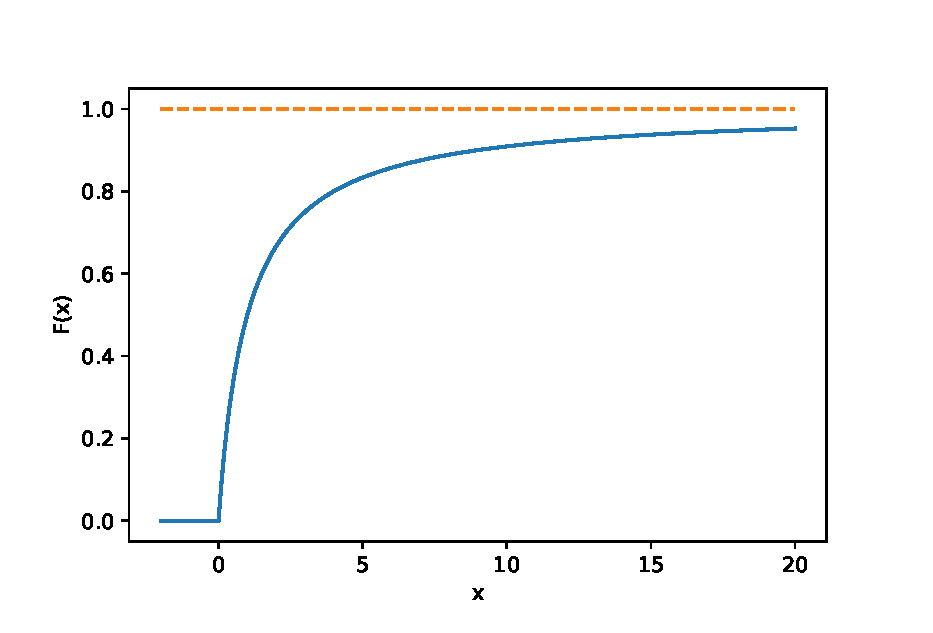
\includegraphics[width=120mm]{Q2A.eps}
\end{center}
ب) تابع \lr{CDF} باید از راست پیوسته باشد؛ در نتیجه $k=1$ و در این صورت تابع مورد نظر، به فرم توزیع تجمعی در می آید.

پ) برای تایع توزیع تجمعی $F$ باید داشته باشیم:
$$
F(-\infty)=0\quad,\quad F(\infty)=1
$$
برای تابع 
$
{e^x+k\over e^x+1}
$
داریم:
$$
F(-\infty)=k\quad,\quad F(\infty)=1
$$
در نتیجه $k=0$. بنابراین تابع \lr{CDF} به صورت زیر است:
\begin{center}
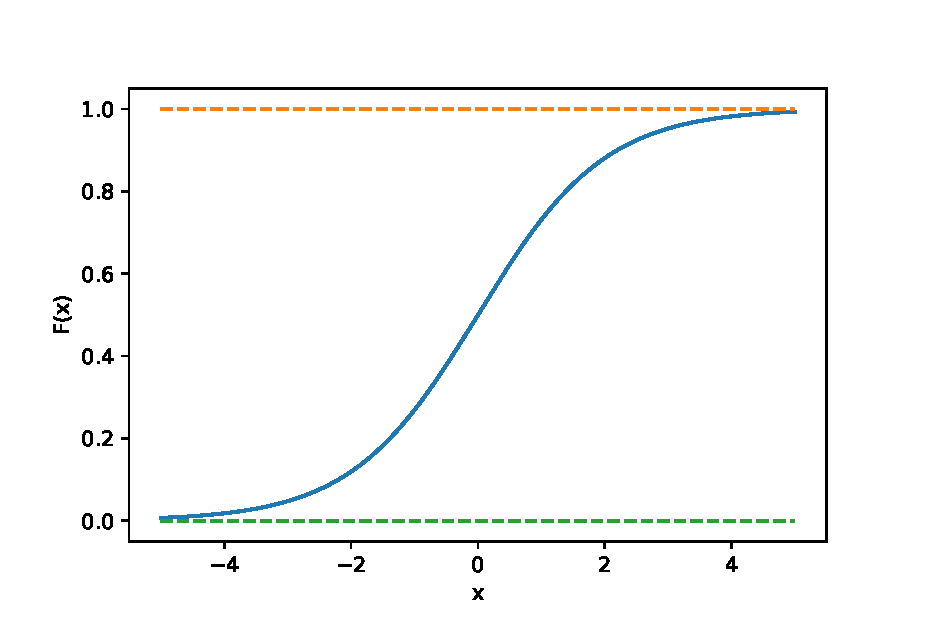
\includegraphics[width=120mm]{Q2B.eps}
\end{center}
ت) یا استدلالی مشابه قسمت قبل و با میل دادن $x$ به $+\infty$ خواهیم داشت $k=1$. در این صورت شکل تابع، به صورت زیر است:
\begin{center}
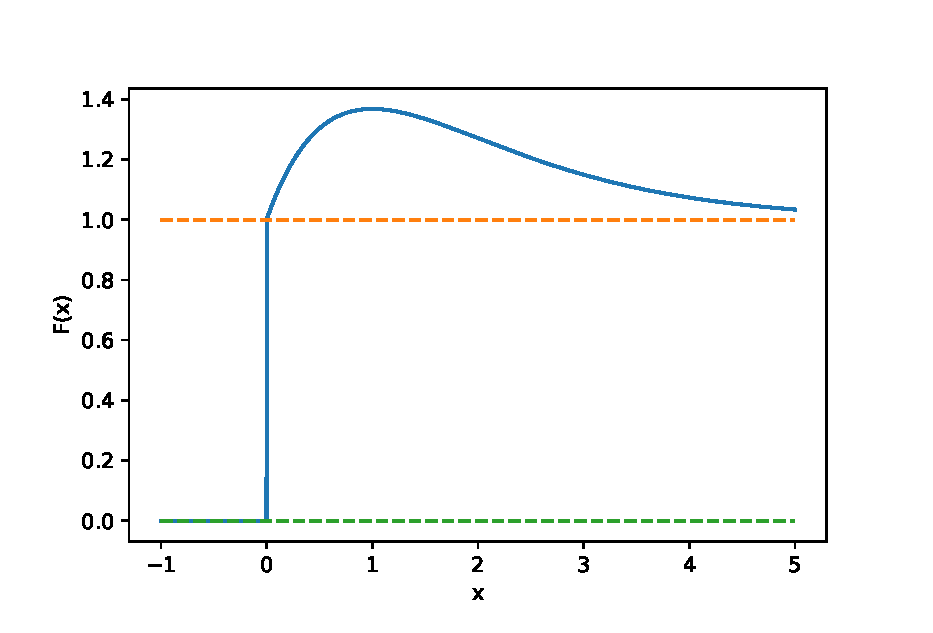
\includegraphics[width=120mm]{Q2C.eps}
\end{center}
مشاهده می شود که تابع به ازای مقادیر مثبت، مقادیر بیشتر از یک را اختیار می کند. در نتیجه تابع نمی تواند \lr{CDF} باشد.

سوال 3) طبق تعریف، میانه صدک 50 محسوب می شود و برای پیدا کردن آن، نیازمند حل معادله ی زیر هستیم:
$$
F(x)={1\over 2}
$$
 که مقدار $x=\ln2$ را برای میانه به دست می دهد.

سوال 4) طبق تعریف
$$
\Pr\{X=x\}=F(x)-F(x^-)
$$
الف)
\eqn{
&F(1)={3\over 4}
\\&F(1^-)={1\over 2}
\\&\implies
\\&\Pr\{X=1\}=F(1)-F(1^-)={1\over 4}
}{}
ب)
\eqn{
&F(1)={1\over 2}
\\&F(1^-)={1\over 2}
\\&\implies
\\&\Pr\{X=1\}=F(1)-F(1^-)=0
}{}
سوال 5) \lr{CDF} را با $G(x)$ و \lr{PDF} را با $g(x)$ نشان می دهیم.

الف)
\eqn{
G(x)&=\Pr\{X+1\le x\}
\\&=\Pr\{X\le x-1\}
\\&=F(x-1)
}{}
در نتیجه
$$
g(x)=f(x-1)
$$
ب)
\eqn{
G(x)&=\Pr\{2X\le x\}
\\&=\Pr\left\{X\le {x\over 2}\right\}
\\&=F\left({x\over 2}\right)
}{}
در نتیجه
$$
g(x)={1\over 2}f\left({x\over 2}\right)
$$
پ)
\eqn{
G(x)&=\Pr\{-X\le x\}
\\&=\Pr\left\{X\ge -x\right\}
\\&=1-\Pr\left\{X< -x\right\}
\\&=1-\Pr\left\{X\le-x\right\}+\Pr\left\{X=-x\right\}
\\&=1-F(-x)+\Pr\left\{X=-x\right\}
}{}
بنابراین
$$
g(x)=f(-x)+{d\over dx}\Pr\left\{X=-x\right\}
$$
جمله ی ${d\over dx}\Pr\left\{X=-x\right\}$ شامل مشتق تابع توزیع تجمعی در ناپیوستگی هاست.

ت)
\eqn{
G(x)&=\Pr\{X^2\le x\}
\\&=\Pr\left\{-\sqrt x\le X\le \sqrt x\right\}
\\&=\Pr\left\{X\le \sqrt x\right\}-\Pr\left\{X<-\sqrt x\right\}
\\&=\Pr\left\{X\le \sqrt x\right\}-\Pr\left\{X\le-\sqrt x\right\}
\\&+\Pr\left\{X=-\sqrt x\right\}
\\&=F(\sqrt x)-F(-\sqrt x)+\Pr\left\{X=-\sqrt x\right\}
}{}
که از روی آن می توان \lr{PDF} را به صورت زیر به دست آورد:
$$
g(x)={1\over 2\sqrt x}\left[f(\sqrt x)+f(-\sqrt x)\right]+{d\over dx}\Pr\left\{X=-\sqrt x\right\}
$$
سوال 6)

الف) خودروها زمانی بدون مشکل از بزرگراه رد می شوند که هر 9 تای آنها بخواهند رد شوند. این احتمال برابر $p^9$ است؛ لذا احتمال مطلوب برابر $1-p^9$ خواهد بود.

ب) 
$$
1-p^9<0.002\implies p\gtrapprox 0.9998
$$
سوال 7) قضیه ی دوموآو-لاپلاس بیان می دارد:
\eqn{
\binom{n}{k}p^k(1-p)^{n-k}\approx G\left({k-np\over\sqrt{np(1-p)}}\right)
}{}
زمانی که $k$ بسیار به $n$ نزدیک و $n$ بسیار بزرگ باشد. از جمله نتایجی که می توان از این قضیه گرفت، عبارتست از:
\eqn{
\sum_{k=k_1}^{k_2}\binom{n}{k}p^k(1-p)^{n-k}\approx
G\left({k_2-np\over\sqrt{np(1-p)}}\right)
-
G\left({k_1-np\over\sqrt{np(1-p)}}\right)
}{}
در این سوال:
$$
p={1\over 2}
$$
بنابراین
\eqn{
\Pr\left\{0.49\le{k\over n}\le0.51\right\}&=
\sum_{0.49n}^{0.51n}\binom{n}{k}p^k(1-p)^{n-k}
\\&\approx
G\left({0.01n\over\sqrt{n\over 4}}\right)
-
G\left({-0.01n\over\sqrt{n\over 4}}\right)
\\&=
2G\left({0.02\sqrt n}\right)-1
\\&>0.95
}{}
در نتیجه
$$
G\left({0.02\sqrt n}\right)>0.975
$$

\QA

دو حالت در نظر می‌گیریم:

حالت 1) لینک DZ خراب باشد. در این صورت، احتمال وجود مسیر بین A و Z برابر است با
$$
p[1-(1-p)(1-p^2)^2]=p-p(1-p)(1-p^2)^2
$$

حالت 2) لینک DZ سالم باشد. در این صورت، می‌توان نودهای D و Z را یکی در نظر گرفت (چرا که رسیدن به D، رسیدن به Z را نتیجه می‌دهد). در این صورت، احتمال وجود مسیر بین A و Z برابر است با
\eqn{
&1-(1-p)\left\{1-\left[1-(1-p)^2\right]\left[1-(1-p)(1-p^2)\right]\right\}
\\&=1-(1-p)\left\{1-(2p-p^2)(p+p^2-p^3)\right\}
\\&=p+p^2(1-p)(2-p)(1+p-p^2)
}{}
در نتیجه، احتمال وجود داشتن مسیر از A تا Z برابر است با
\eqn{
&
(1-p)[p+p^2(1-p)(2-p)(1+p-p^2)]+p^2+p^3(1-p)(2-p)^2
\\&=
p+p^2(1-p)^2(2-p)(1+p-p^2)+p^3(1-p)(2-p)^2
}{}

%حالت 1) لینک CD خراب باشد. در این صورت، احتمال وجود مسیر بین A و Z برابر است با
%$$
%1-(1-p^2)\left[1-p(1-p)(1-p^2)\right]
%$$
%
%اگر هر دو لینک CZ و DZ خراب باشند، مسیری از A تا Z وجود ندارد. در نتیجه، باید حداقل یک لینک از این 2 لینک سالم باشد. سه حالت ممکن است:
%
%1) لینک CZ سالم و لینک DZ خراب باشد.
%
%2) لینک CZ خراب و لینک DZ سالم باشد.
%
%3) لینک CZ سالم و لینک DZ سالم باشد.
%
%در حالت اول، پیشامد وجود داشتن مسیر از A تا Z، معادل با وجود داشتن مسیر از A تا C است. مکمل پیشامد اخیر، وجود نداشتن مسیر از A تا C است. چون از A تا C سه مسیر وجود دارد، هر سه باید خراب باشند. خراب بودن هر مسیر، مکمل سالم بودن آن است که سالم بودن هر مسیر نیز، سالم بودن تمام لینک‌های آن را می‌طلبد. با توضیحات پیش، برای محاسبه‌ی احتمال وجود داشتن مسیر از A تا C، مشروط بر اینکه لینک CZ سالم و لینک DZ خراب باشد، برابر است با
%$$
%1-(1-p^2)(1-p)(1-p^2).
%$$
%
%در حالت دوم، پیشامد وجود داشتن مسیر از A تا Z، معادل با وجود داشتن مسیر از A تا D است. احتمال این پیشامد، به طریق مشابه برابر است با
%$$
%1-(1-p)\left\{1-p\left[1-(1-p)(1-p^2)\right]\right\}.
%$$
%
%حالت سوم، معادل این است که دو نود C و D را به هم بچسبانیم (و لینک CD را از بین ببریم). در این صورت، احتمال وجود مسیر از A تا نود C (که همان D است) برابر است با
%$$
%1-(1-p)^2(1-p^2).
%$$
%
%در نتیجه، احتمال وجود مسیر از A تا Z به صورت زیر است:
%\eqn{
%p(1-p)[1-(1-p^2)(1-p)(1-p^2)+1-(1-p)\left\{1-p\left[1-(1-p)(1-p^2)\right]\right\}]
%}{}
%
%ابتدا باید تمام پیشامدها (مسیرها)ی ممکن از A تا Z را پیدا کنیم. با شمارش ساده‌ای، این مسیرها عبارتند از:
%
%ABCZ
%
%ACZ
%
%ADCZ
%
%ABCDZ
%
%ACDZ
%
%ADZ
%
%احتمال سالم بودن این مسیرها، به ترتیب برابراست با
%
%$
%p^3
%$
%
%$
%p^2
%$
%
%$
%p^3
%$
%
%$
%p^4
%$
%
%$
%p^3
%$
%
%$
%p^2
%$
%
%و احتمال مطلوب (معادل با سالم بودن حداقل یک مسیر از )

%\begin{figure}[h]
%\centering
%\includegraphics[width=50mm]{PS7_ProbStat_Q1.eps}
%\end{figure}

\QA

الف)
$$
\binom{10}{3}(\frac{1}{2})^3(\frac{1}{2})^7=\frac{120}{1024}
$$

ب) مکمل پیشامد مطلوب، آن است که دقیقا 1 یا صفر بار خط بیاید. در نتیجه احتمال مطلوب برابر است با
$$
1-\binom{10}{0}(\frac{1}{2})^0(\frac{1}{2})^{10}-\binom{10}{1}(\frac{1}{2})^1(\frac{1}{2})^9=1-\frac{1}{1024}-\frac{10}{1024}=\frac{1013}{1024}
$$

پ) اگر بدانیم در 5 پرتاب اول خط آمده است، احتمال مطلوب، معادل با احتمال رو آمدن دقیقأ دو خط در 5 پرتاب باقیمانده است. در نتیجه احتمال مطلوب برابر است با
$$
\binom{5}{2}(\frac{1}{2})^2(\frac{1}{2})^3=\frac{10}{32}
.
$$
از روش احتمال شرطی نیز به همین پاسخ می‌رسیم.

\QA

الف) جمع این 6 پرتاب زمانی 8 می‌شود که یا دقیقأ دو بار 2 و 4 بار 1 یا دقیقا یک بار 3 و 5 بار 1 داشته باشیم. در این صورت، احتمال مطلوب برابر است با
$$
\binom{6}{2}(\frac{1}{6})^2(\frac{1}{6})^4
+
\binom{6}{1}(\frac{1}{6})^1(\frac{1}{6})^5
=\frac{21}{46656}
$$

ب)
$$
\frac{6!}{6^6}=\frac{5!}{6^5}=\frac{5}{324}
$$

\QA

احتمال آبی بودن توپ در هر آزمایش، برابر
$
0.7
$
است. چون توپ در هر مرحله به کیسه باز می‌گردد، آزمایش ها مستقلند و در نتیجه، احتمال مطلوب برابر است با
$$
\binom{11}{7}(0.7)^7(0.3)^4
$$

\QA

چنانچه حداکثر 10 کاربر بخواهند به طور همزمان از کانال استفاده کنند، کمبود پهنای باند نخواهیم داشت. بنابراین احتمال مطلوب برابر است با
\eqn{
\sum_{k=0}^{10} \binom{12}{k}(0.6)^k(0.4)^{12-k}&=
1-\sum_{k=11}^{12} \binom{12}{k}(0.6)^k(0.4)^{12-k}
\\&=
1-12(0.6)^{11}(0.4)-(0.6)^{12}
\\&\approx0.9804
}

\QA

مطلوب آن است که مقدار 
$
P\left\{\frac{97}{300}<\frac{k}{n}<\frac{103}{300}\right\}
$،
حداقل $99\%$ باشد. با تقریب دموآور لاپلاس خواهیم داشت:
$$
2G(\epsilon\sqrt{\frac{n}{p(1-p)}})-1\ge 0.99
$$
که در آن
$
\epsilon=0.01
$
و
$
p=\frac{1}{3}
$.
در نتیجه
\eqn{
&\quad\quad\quad G(0.01\sqrt{\frac{n}{\frac{2}{9}}})\ge 0.995
\\&\implies
0.01\sqrt{\frac{n}{\frac{2}{9}}}\ge G^{-1}(0.995)
\\&\implies
0.01\sqrt{\frac{n}{\frac{2}{9}}}\gtrapprox 2.5758
\\&\implies
n\ge 14745
}

\chapter{متغیرهای تصادفی}

سوال 1) الف) 
$$
\binom{n}{k}p^k(1-p)^{n-k}=0.2668\quad,\quad e^{-np}{(np)^k\over k!}=0.1490\quad,\quad \text{Rel. Err.}= 44.16\%
$$

ب)
$$
\binom{n}{k}p^k(1-p)^{n-k}=0.1573\quad,\quad e^{-np}{(np)^k\over k!}=0.1318\quad,\quad \text{Rel. Err.}= 16.23\%
$$

پ)
$$
\binom{n}{k}p^k(1-p)^{n-k}=0.3716\quad,\quad e^{-np}{(np)^k\over k!}=0.3679\quad,\quad \text{Rel. Err.}= 1\%
$$

مشاهده می شود که در حالت سوم، خطای تقریب از همه کم تر است؛ زیرا شرایطی که باعث افزایش دقت تقریب می شوند ($n>>1$ و $k\approx np$)، در این حالت به خوبی مراعات شده اند.

سوال 2) در پرتاب دو تاس سالم، اگر متغیر تصادفی $X$ را برابر تعداد اعداد زوج رو آمده در هر دو تاس در نظر بگیریم:

الف) 
$$
\Omega=\{0,1,2\}
$$

ب) با توجه به فضای شدنی X، داریم:
$$
\Pr\{X\le1.5\}=\Pr\{X=0\text{ یا } X=1\}=\Pr\{X=0\}+\Pr\{X=1\}
$$
و
$$
\Pr\{X\le0.5\}=\Pr\{X=0\}
$$
بنابراین 
$$
\Pr\{X\le1.5\}-\Pr\{X\le0.5\}=\Pr\{X=1\}=\binom{2}{1}\times {3\over 6}\times {3\over 6}={1\over 2}
$$

پ)
$$
p_X(x)=\Pr\{X=x\}=
\begin{cases}
{1\over 4}&,\quad x=0,2\\
{1\over 2}&,\quad x=1
\end{cases}
$$

سوال 3) فرض کنید یک سکه سالم را n بار پرتاب کرده ایم. در اینصورت pmf متغیر تصادفی X را در حالت های زیر بیابید.

الف) متغیر تصادفی X برابر تعداد روها در پرتاب های زوج است. 

$$
\Pr\{X=x\}=\binom{\lfloor{n\over 2}\rfloor}{x}\left({1\over 2}\right)^{\lfloor{n\over 2}\rfloor}
$$

ب) متغیر تصادفی X فقط 5 مقدار 
$
\{0,1,2,3,4\}
$
را با احتمال غیرصفر اختیار می کند؛ بنابراین
$$
p_X(x)=\Pr\{X=x\}=
\binom{4}{x}{1\over 16}
$$

پ) اگر n فرد باشد، تعداد روها و پشت ها هرگز برابر نمی شوند؛ پس 
$$
\Pr\{X=x\}=\begin{cases}
1&,\quad x=0\\
0&,\quad x=1
\end{cases}
$$
و برای n زوج
$$
\Pr\{X=x\}=\begin{cases}
1-\binom{n}{{n\over 2}}\left({1\over 2}\right)^n&,\quad x=0\\
\binom{n}{{n\over 2}}\left({1\over 2}\right)^n&,\quad x=1
\end{cases}
$$

سوال 1) الف)
\eqn{
E\{X\}&=\int_{-\infty}^{\infty}{xf(x)}dx
\\&=
\int_{a}^{b}{x\over b-a}dx
\\&=
{1\over b-a}{b^2-a^2\over 2}
\\&=
{b+a\over 2}
}{}
هم چنین
\eqn{
\sigma_X^2=E\{X^2\}-E^2\{X\}
}{}
و
\eqn{
E\{X^2\}&=\int_{-\infty}^{\infty}{x^2f(x)}dx
\\&=
\int_{a}^{b}{x^2\over b-a}dx
\\&=
{1\over b-a}{b^3-a^3\over 3}
\\&=
{b^2+a^2+ab\over 3}
}{}
در نتیجه
\eqn{
\sigma_X^2&={b^2+a^2+ab\over 3}-{b^2+a^2+2ab\over 4}
\\&
={1\over 12}(4a^2+4b^2+4ab-3a^2-3b^2-6ab)
\\&
={(b-a)^2\over 12}
}{}
ب)
\eqn{
E\{X\}&=\int_0^\infty {x\over \lambda}e^{-{x\over \lambda}}dx
\\&=
\lambda\int_0^\infty xe^{-x}dx
\\&=
\lambda\left[-xe^{-x}\Big|_0^\infty+\int_0^\infty e^{-x}dx\right]
\\&=
\lambda
}{}
همچنین به کمک انتگرال جزء به جزء
\eqn{
E\{X^2\}&=\int_0^\infty {x^2\over \lambda}e^{-{x\over \lambda}}dx
\\&=
\lambda^2\int_0^\infty x^2e^{-x}dx
\\&=
\lambda^2\left[-x^2e^{-x}\Big|_0^\infty+2\int_0^\infty xe^{-x}dx\right]
\\&=
2\lambda^2
}{}
بنابراین
\eqn{
\sigma_X^2=\lambda^2
}{}
پ)
\eqn{
E\{X\}=\sum nf(n)=p\times 0+(1-p)\times 1=1-p
}{}
هم چنین
\eqn{
E\{X^2\}=\sum n^2f(n)=p\times 0^2+(1-p)\times 1^2=1-p
}{}
بنابراین
$$\sigma_X^2=p(1-p)$$
ت) ابتدا می دانیم
$$
\sum_{n=0}^\infty e^{-\lambda}{\lambda^n\over n!}=1
$$
بنابراین
\eqn{
E\{X\}&=
\sum_{n=0}^\infty n\cdot e^{-\lambda}{\lambda^n\over n!}
\\&=
\sum_{n=1}^\infty n\cdot e^{-\lambda}{\lambda^n\over n!}
\\&=
\sum_{n=1}^\infty e^{-\lambda}{\lambda^n\over (n-1)!}
\\&=
\sum_{n=0}^\infty e^{-\lambda}{\lambda^{n+1}\over n!}
\\&=
\lambda\sum_{n=0}^\infty e^{-\lambda}{\lambda^{n}\over n!}
\\&=\lambda
}{}
هم چنین
\eqn{
E\{X^2\}&=
\sum_{n=0}^\infty n^2\cdot e^{-\lambda}{\lambda^n\over n!}
\\&=
\sum_{n=1}^\infty n^2\cdot e^{-\lambda}{\lambda^n\over n!}
\\&=
\sum_{n=1}^\infty n\cdot e^{-\lambda}{\lambda^n\over (n-1)!}
\\&=
\sum_{n=1}^\infty (n-1+1)\cdot e^{-\lambda}{\lambda^n\over (n-1)!}
\\&=
\sum_{n=1}^\infty (n-1)\cdot e^{-\lambda}{\lambda^n\over (n-1)!}
+
\sum_{n=1}^\infty e^{-\lambda}{\lambda^n\over (n-1)!}
\\&=
\sum_{n=2}^\infty (n-1)\cdot e^{-\lambda}{\lambda^n\over (n-1)!}
+
\lambda
\\&=
\sum_{n=2}^\infty e^{-\lambda}{\lambda^n\over (n-2)!}
+
\lambda
\\&=
\lambda^2\sum_{n=0}^\infty e^{-\lambda}{\lambda^n\over n!}
+
\lambda
\\&=
\lambda+\lambda^2
}{}
بنابراین
\eqn{
\sigma_X^2=\mu_X=\lambda
}{}

سوال 2) فرض کنیم متغیر تصادفی $X$، تعداد پرتاب ها تا رخداد $k$ امین موفقیت  باشد. بنابراین پیشامد $X=n$ معادل است با اینکه بگوییم در $n$ امین پرتاب، به $k$ امین موفقیت می رسیم. همچنین می توان گفت که در $n-1$ پرتاب قبلی، دقیقا به $k-1$ موفقیت دست یافته ایم که این، طبق توزیع دو جمله ای با احتمال 
$
\binom{n-1}{k-1}p^{k-1}(1-p)^{n-k}
$
 رخ می دهد. چون احتمال موفقیت در پرتاب $n$ ام نیز برابر $p$ است، داریم
\eqn{
\Pr\{X=n\}=\binom{n-1}{k-1}p^{k}(1-p)^{n-k}\quad,\quad n\ge k
}{}
اکنون متوسط تعداد پرتاب ها را حساب می کنیم.

الف) $k=1$
\eqn{
\Pr\{X=n\}=p(1-p)^{n-1}\quad,\quad n\ge 1
}{}
از یک اتحاد ساده استفاده می کنیم (که به کمک مشتق می توان آن را نشان داد. در اینجا آن را بدون اثبات رها می کنیم)
\eqn{
\sum_{n=1}^\infty n\cdot u^{n-1}={1\over (1-u)^2}
}{}
بنابراین
\eqn{
E\{X\}=\sum_{n=1}^\infty np(1-p)^{n-1}={1\over p}
}{}
ب) $k=2$
\eqn{
\Pr\{X=n\}=(n-1)p^2(1-p)^{n-2}\quad,\quad n\ge 2
}{}
این بار به کمک اتحاد زیر (با مشتق گیری از اتحاد قبلی!)
\eqn{
\sum_{n=2}^\infty n(n-1)\cdot u^{n-2}={2\over (1-u)^3}
}{}
خواهیم داشت
\eqn{
E\{X\}=\sum_{n=2}^\infty n(n-1)p^2(1-p)^{n-2}={2\over p}
}{}

سوال 3) هنگامی که به طور متوسط از معیارهای کمی برای ارزیابی یک جامعه ی بزرگ استفاده می شود، می توان گفت که میانگین، مهم ترین معیار کمی ارزیابی است؛ به عبارت دیگر اگر به هریک از افراد یک جامعه، نمره‌ی مخصوصی داده شود، ارزیابی کلی جامعه مستلزم محاسبه کرد میانگین نمرات تکی افراد است. البته که میانگین، تنها کمیت ارزیابی مهم نیست و به طور مثال واریانس نیز معیار بسیار مهم دیگری به شمار می رود. به طور شهودی میانگین، میزان برتری نسبی یک جامعه را به دیگری نشان می دهد. واریانس، نشان دهنده ی میزان یکنواختی افراد جامعه است. طبق این توضیحات، 
\textbf{
افراد جامعه ای با متوسط نمرات 73 به لحاظ سطح علمی بالاترند؛ اما جامعه ای با میانگین 59 و واریانس 9، دارای افراد هم سطح تری است.
}

سوال 4) الف) مسلما دامنه‌ی تعریف چنین چگالی احتمالی متقارن است و داریم
$$
\forall x\in D\quad,\quad f(-x)=-f(x)
$$
چون تابع چگالی احتمال نامنفی است، در نتیجه باید الزاما داشته باشیم
$$
\forall x\in D\quad,\quad f(x)=0
$$
می توان گفت چنین توزیعی وجود ندارد؛ اما در بسیاری از متون ریاضی، از آن به عنوان 
\textbf{
توزیع گوسی با واریانس بینهایت
}
 نام می برند.

ب)
\eqn{
E\{X^n\}&=\int_{-\infty}^\infty {x^n}f(x)dx
\\&=\int_{a}^b {x^n\over b-a}dx
\\&={b^{n+1}-a^{n+1}\over nb-na}
}{}

سوال 5)
 الف) بررسی درستی این موضوع کار ساده ای است؛ زیرا پیشامد های 
$
e^{sX}\ge e^{sa}
$
 و 
$
X\ge a
$
 معادلند؛ به عبارت دیگر از هر یک می توان دیگری را نتیجه گرفت.

ب) طبق فرایند مارکوف برای یک متغیر تصادفی مثبت $Y$ و $b>0$
$$
\Pr\{Y\ge b\}\le{E\{Y\}\over b}
$$
بنابراین با تعریف $Y=e^{sX}$ و $b=e^{sa}$ خواهیم داشت:
$$
\Pr\{X\ge a\}=\Pr\{e^{sX}\ge e^{sa}\}\le{E\{e^{sX}\}\over e^{sa}}
$$
به کمک تعریف تابع مولد گشتاور به صورت 
$
\phi_X(s)\triangleq E\{e^{sX}\}
$،
 نتیجه ی مورد نظر فورا حاصل می شود.

سوال 1) هر CDF باید سه خاصیت داشته باشد:
\[
\begin{split}
&F(-\infty)=0
\\&F(\infty)=1
\\&F(x) \text{صعودی}
\end{split}
\]
الف) شرط 
$
F(\infty)=1
$
هنگامی برآورده می شود که 
$$
\lim_{x\to \infty}1-e^{-kx^2}=1\implies k>0
$$
از طرفی به ازای هر 
$
k>0
$
، تابع 
$
1-e^{-kx^2}
$
روی مقادیر 
$
x>0
$
صعودی است؛ پس محدوده‌ی مناسب $k$، 
$
(0,\infty)
$
خواهد بود.

ب) صعودی بودن $F(x)$ الزام می دارد که 
$
k\ge 0
$. از طرفی، نباید مقدار CDF هیچ کجا از بازه‌ی $[0,1]$ تجاوز کند. در این صورت 
$
k\le 1
$
. 
همچنان یک شرط دیگر باید برآورده شود و آن پیوستگی از راست CDF در تمام نقاط است. این نوع پیوستگی در $x=1$ تنها زمانی رخ می دهد که $k=1$. پس بازه‌ی مناسب $k$ برابر 
$
\{1\}
$
است.

پ) از آنجا که 
$
F(\infty)=1
$
، باید داشته باشیم 
$
k=1
$
؛ ولی صعودی بودن $F(x)$ نقض می شود؛ زیرا
$$
0<x<{1\over 2}\implies x-x^2 \text{صعودی اکید}\implies e^{x-x^2}\text{صعودی اکید}\implies 1-e^{x-x^2}\text{نزولی اکید}
$$
پس در این مورد، k هیچ مقداری را نمی تواند داشته باشد.

ت) شرایط 
$
F(-\infty)=0
$
و
$
F(\infty)=1
$
به ازای 
$
k\ne0
$
برآورده می شوند. صعودی بودن نیز به ازای 
$
k\ge0
$
رخ می دهد؛ پس بازه‌ی مناسب برابر است با 
$
(0,\infty)
$
.

ث) با توجه به اینکه 
$
F(-\infty)=\cos{\pi\over k}=0
$
باید داشته باشیم
$$
{\pi\over k}=l\pi+{\pi\over 2}\implies k={2\over 2l+1}\quad,\quad l\in \Bbb Z
$$
از طرفی چون به ازای 
$
k<0
$
، تابع 
$
{\pi\over e^x+k}
$
دارای مجانب عمودی خواهد بود، بنابراین باید داشته باشیم
$$
k={2\over 2l+1}\quad,\quad l\in \Bbb Z^{\ge 0}
$$
%$
%
%$

سوال 2) الف) $F(x^2)$ در $-\infty$ دارای مقدار 1 (بجای 0) می شود؛ پس نمی‌تواند CDF باشد.

ب، پ، ت و ث) این توابع تمام شرایط CDF را برآورده می کنند.

سوال 3) با توجه به جبر مجموعه ها، با تعریف
$$
A=(-\infty,2]
$$
$$
B=(-\infty,1]
$$
خواهیم داشت
$$
\Pr\{1<x\le 2\}=\Pr\{A-B\}=\Pr\{A\}-\Pr\{B\}=F(2)-F(1)
$$
الف)
$$
\Pr\{1<x\le 2\}=e^{-k}-e^{-4k}
$$
ب)
$$
\Pr\{1<x\le 2\}=0
$$
پ) (!!)

ت) 
$$
\Pr\{1<x\le 2\}={e^2\over e^2+k}-{e\over e+k}
$$
ث)
$$
\Pr\{1<x\le 2\}=\cos {\pi\over e^2+k}-\cos {\pi\over e+k}
$$

{\color{red}
نکته مهم:
$$
\int_a^b\delta(x-c)dx=\begin{cases}
1&,\quad a<c<b\\
0&,\quad \text{در غیر این صورت}
\end{cases}
$$
}

سوال 1) الف) به وضوح باید $k$ مثبت باشد در غیر این صورت این تابع همواره سطح زیر نامحدود خواهد داشت. از طرفی
$$
\int_{-\infty}^\infty f(x)dx=\int_1^\infty {1\over x^k}dx=\begin{cases}
\infty&,\quad0<k\le1\\
{1\over k-1}&,\quad k>1
\end{cases}
$$
پس $k=2$.

ب) این تابع نیز تمام شرایط pdf را برآورده می کند؛ به شرط آن که سطح زیر آن واحد باشد. در این صورت:
$$
\int_{-\infty}^\infty f(x)dx=\int_0^\infty kxe^{-x}dx=-k(x+1)e^{-x}|_0^\infty=k=1
$$
پس k فقط باید برابر 1 باشد.

پ) به ازای $k>\pi$، pdf مقادیر منفی را نیز اختیار می کند؛ پس $k\le \pi$. از طرفی
$$
\int_{-\infty}^\infty f(x)dx=\int_0^k\sin xdx=1-\cos k=1
$$
پس $k={\pi\over 2}$.

ت)
$
f(x)=\begin{cases}
k\delta(x-1)&,\quad x=1\\
x&,\quad 0<x<1\\
0&,\quad \text{سایر جاها}
\end{cases}
$
(به عبارت دیگر، تابع در نقطه‌ی $x=1$ دارای ضربه‌ای به مساحت k است)
ابتدا باید $k$ مثبت باشد تا مقدار چگالی احتمال همواره نامنفی باشد. همچنین
$$
\int_{-\infty}^\infty f(x)dx=\int_{1^-}^{1^+} k\delta(x-1)dx+\int_0^1 xdx=k+0.5=1
$$
پس مقدار k باید برابر $0.5$ باشد.

ث) سطح زیر این چگالی همواره برابر 1 است و فقط هنگامی نامنفی می شود که 
$
0\le k\le 1
$.

سوال 2) مکمل این حالت زمانی رخ می دهد که بیش از 65 قطعه خراب شوند. احتمال خرابی هر قطعه در بازه‌ی $
\left(0,{T\over 4}\right)
$
برابر است با:
$$
p=\int_{-\infty}^{T\over 4}f(x)dx=
\int_{0}^{T\over 4}{1\over T}e^{-{x\over T}}dx=
\int_{0}^{1\over 4}e^{-x}dx=1-e^{-0.25}
$$
بنابراین احتمال پیشامد مطلوب برابر است با:
\[
\begin{split}
P&=1-[\binom{70}{66}p^{66}(1-p)^4\\&+\binom{70}{67}p^{67}(1-p)^3
+\binom{70}{68}p^{68}(1-p)^2
\\&+\binom{70}{69}p^{69}(1-p)
+\binom{70}{70}p^{70}
]
\end{split}
\]

سوال 3) اگر تابع توزیع تجمعی را با $F(x)$ نشان دهیم در این صورت:
$$
\Pr\{X=1\}=F(1)-F(1^-)
$$
\[
\begin{split}
\Pr\{X<{1\over 2}\}&=\Pr\{X\le{1\over 2}\}-\Pr\{X={1\over 2}\}\\&=F(0.5)-[F(0.5)-F(0.5^-)]=F(0.5^-)
\end{split}
\]
الف)
$$
\Pr\left\{X<{1\over 2}\right\}=0\quad ,\quad \Pr\{X=1\}=0
$$
ب)
$$
\Pr\left\{X<{1\over 2}\right\}=1-{3\over 2}e^{-{1\over 2}}\quad ,\quad \Pr\{X=1\}=0
$$
پ)
$$
\Pr\left\{X<{1\over 2}\right\}=1-\cos{1\over 2}\quad ,\quad \Pr\{X=1\}=0
$$
ت)
$$
\Pr\left\{X<{1\over 2}\right\}={1\over 8}\quad ,\quad \Pr\{X=1\}={1\over 2}
$$
ث)
$$
\Pr\left\{X<{1\over 2}\right\}=1-k\quad ,\quad \Pr\{X=1\}=k
$$

سوال 4) طبق تعریف، برای صدک-u داریم:
$$
x_u=\inf\{x\ \ |\ \ F(x)=y\}
$$
که $F(x)$ تابع توزیع تجمعی متغیر تصادفی است. به طور ساده تر، باید معادله‌ی 
$
F(x_u)=u
$
را حل کنیم. بنابراین:

الف)
$$
F(x)=\begin{cases}
1&,\quad 0\le x\le 1\\
x&,\quad x>1\\
0&,\quad x<0
\end{cases}
$$
و در نتیجه
$
x_u=u
$
.

ب)
$$
F(x)=\begin{cases}
0&,\quad x<0\\
1-e^{-2x}&,\quad x\ge 0
\end{cases}
$$
پس
$
x_u={1\over 2}\ln {1\over 1-u}
$

{\color{red}
نکته مهم:
$$
\int_a^b\delta(x-c)dx=\begin{cases}
1&,\quad a<c<b\\
0&,\quad \text{در غیر این صورت}
\end{cases}
$$
}

سوال 1) الف) 
$$
P=\int_0^{2\lambda}{1\over \lambda}e^{-{x\over\lambda}}dx
=\int_0^{2}e^{-x}dx=1-e^{-2}\approx0.86
$$

ب) 
$$
P=\int_{3\lambda}^{3.5\lambda}{1\over \lambda}e^{-{x\over\lambda}}dx
=\int_3^{3.5}e^{-x}dx=e^{-3}-e^{-3.5}\approx0.02
$$

سوال 2) الف)
$$
\int_{-\infty}^\infty f_X(x)dx=\int_0^16x^2(1-x)dx+\int_{-\infty}^{\infty}k\delta(x+1)dx={1\over2}+k=1
$$
پس
$
k={1\over 2}
$
.

ب)
$$
F(x)=\int_{-\infty}^xf(u)du=\begin{cases}
0&,\quad x<-1\\
{1\over 2}&,\quad -1\le x<0\\
{1\over 2}+2x^3-{3\over 2}x^4&,\quad 0\le x<1\\
1&,\quad 1\le x
\end{cases}
$$
\begin{figure}[htbp]
\centering
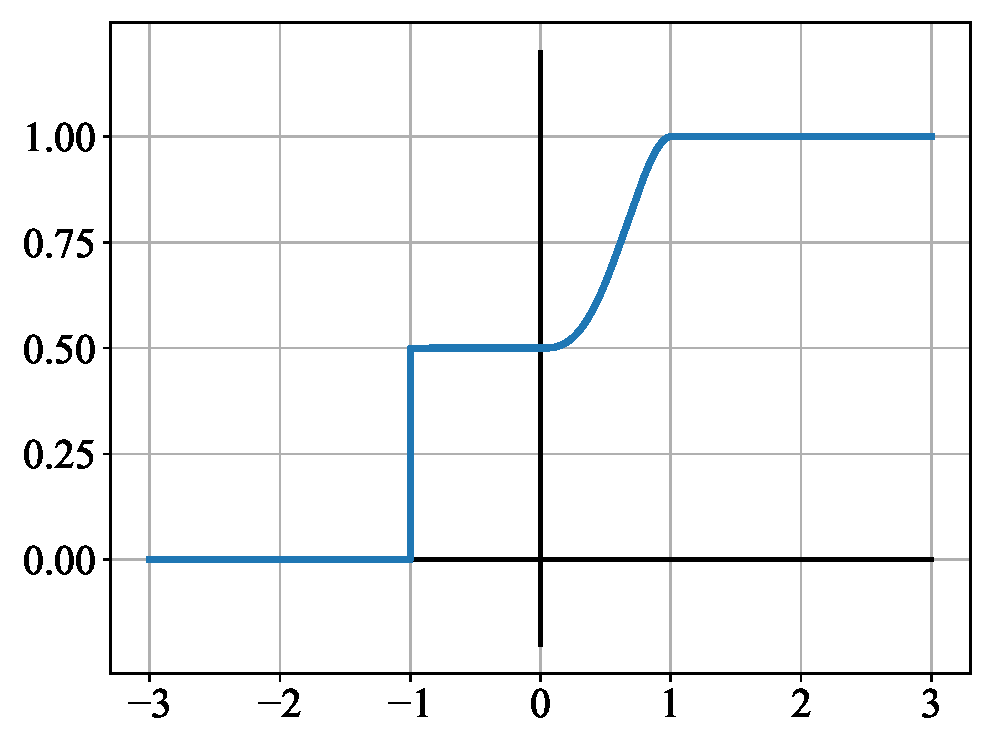
\includegraphics[width=80mm]{CDF_HW9.eps}
\end{figure}

پ)
$$
\Pr\{-2< X\le {1\over2}\}=F(0.5)-F(-2)={21\over 32}\approx0.66
$$
و
$$
\Pr\{0< X\le {1\over2}\}=F(0.5)-F(0)={5\over 32}\approx0.16
$$

سوال 3) الف) اگر $y<0$، در اینصورت مقدار 
$
\Pr\{Y\le y\}
$
همواره برابر صفر است؛ زیرا 
$
Y=X^2
$
نمی تواند منفی باشد. به ازای 
$
y\ge 0
$
:
\[
\begin{split}
\Pr\{Y\le y\}&=\Pr\{X^2\le y\}
=\Pr\{-\sqrt y\le X\le \sqrt y\}
\\&=\Pr\{0\le X\le \sqrt y\}=\begin{cases}
\sqrt y&,\quad y<1\\
1&,\quad y\ge1
\end{cases}
\end{split}
\]
در نتیجه
$$
F_Y(y)=\begin{cases}
0&,\quad y<0\\
\sqrt y&,\quad 0\le y<1\\
1&,\quad y\ge1
\end{cases}
$$
و
$$
f_Y(y)=\begin{cases}
\frac{1}{2\sqrt y}&,\quad 0<y<1\\
0&,\quad \text{سایر جاها}
\end{cases}
$$

ب)
\[
\begin{split}
&\Pr\{Y\le y\}=\Pr\{-\ln(1-X)\le y\}
=\Pr\{\ln (1-X)\ge -y\}
\\&=\Pr\{1-X\ge e^{-y}\}
=\Pr\{X\le 1-e^{-y}\}
=\begin{cases}
0&,\quad 1-e^{-y}\le0\\
1-e^{-y}&,\quad 0<1-e^{-y}<1\\
1&,\quad 1-e^{-y}\ge1
\end{cases}
\\&=\begin{cases}
0&,\quad y\le0\\
1-e^{-y}&,\quad 0<y\\
1&,\quad e^{-y}\le0 {\color{red}\text{(هرگز رخ نمی دهد)}}
\end{cases}
=\begin{cases}
0&,\quad y\le0\\
1-e^{-y}&,\quad 0<y
\end{cases}
\end{split}
\]
عبارت فوق، رابطه‌ی CDF بوده و PDF از مشتق CDF به صورت زیر به دست می آید:
$$
f_Y(y)=
\begin{cases}
0&,\quad y\le0\\
e^{-y}&,\quad 0<y
\end{cases}
$$

پ)
\[
\begin{split}
\Pr\{Y\le y\}&=\Pr\{\tan\pi(X-{1\over 2})\le y\}
=\Pr\{\pi(X-0.5)\le \tan^{-1}y\}
\\&=\Pr\{X-0.5\le {1\over \pi}\tan^{-1}y\}
=\Pr\{X\le {1\over 2}+{1\over \pi}\tan^{-1}y\}
\\&=\begin{cases}
0&,\quad {1\over 2}+{1\over \pi}\tan^{-1}y\le0\\
{1\over 2}+{1\over \pi}\tan^{-1}y&,\quad 0<{1\over 2}+{1\over \pi}\tan^{-1}y<1\\
1&,\quad {1\over 2}+{1\over \pi}\tan^{-1}y\ge1
\end{cases}
\\&=\begin{cases}
0&,\quad y\le-\infty{\color{red}\text{(هرگز رخ نمی دهد)}}\\
{1\over 2}+{1\over \pi}\tan^{-1}y&,\quad -\infty<y<\infty\\
1&,\quad y\ge\infty{\color{red}\text{(هرگز رخ نمی دهد)}}
\end{cases}
\end{split}
\]
پس
$$
F_y(y)={1\over 2}+{1\over \pi}\tan^{-1}y\quad,\quad f_Y(y)={1\over \pi}{1\over 1+y^2}
$$

سوال 4) 
$$
\Pr\{X<{2\over 3}\}=F_X({2\over 3})={2\over 3}
$$
و
$$
\Pr\{Y<{1\over \sqrt3}\}=F_X({1\over \sqrt3})={1\over 2}+{1\over\pi}\tan^{-1}{1\over\sqrt 3}={1\over 2}+{1\over\pi}\times{\pi\over 6}={2\over 3}
$$
دو مقدار احتمال با هم برابرند؛ زیرا تابعی که بین دو متغیر تصادفی برقرار است ($Y=\tan\pi(X-{1\over 2})$)، مقدار 
$
2\over 3
$
را به 
$
{1\over \sqrt 3}
$
نگاشت می دهد. از دیدگاه دیگر، ما دو برداشت متفاوت از یک احتمال را محاسبه کرده ایم.

سوال 5) الف) 
\[
\begin{split}
\Pr\{Y\le y\}&=\Pr\{|X|\le y\}
\\&=\begin{cases}
0&,\quad y<0\\
\Pr\{-y\le X\le y\}&,\quad y\ge 0
\end{cases}
\\&=\begin{cases}
0&,\quad y<0\\
\Pr\{X\le y\}-\Pr\{X<-y\}&,\quad y\ge 0
\end{cases}
\\&=\begin{cases}
0&,\quad y<0\\
F(y)-F(-y^-)&,\quad y\ge 0
\end{cases}
\end{split}
\]

ب) 
$$
\Pr\{Y=0\}=1-\Pr\{Y=1\}=\Pr\{X\le0\}=F(0)
$$
بنابراین
$$
F_Y(y)=\begin{cases}
0&,\quad y<0\\
F(0)&,\quad 0\le y<1\\
1&,\quad y\ge 1
\end{cases}
$$

پ) 
\[
\begin{split}
\Pr\{Y\le y\}&=\Pr\{X^2-2X\le y\}
\\&=\Pr\{X^2-2X+1\le y+1\}
\\&=\Pr\{(X-1)^2\le y+1\}
\\&=\begin{cases}
0&,\quad y+1<0\\
\Pr\{|X-1|\le \sqrt{y+1}\}&,\quad y+1\ge 0
\end{cases}
\\&=\begin{cases}
0&,\quad y<-1\\
\Pr\{1-\sqrt{y+1}\le X\le 1+\sqrt{y+1}\}&,\quad y\ge -1
\end{cases}
\\&=\begin{cases}
0&,\quad y<-1\\
\Pr\{X\le 1+\sqrt{y+1}\}-\Pr\{X< 1-\sqrt{y+1}\}&,\quad y\ge -1
\end{cases}
\\&=\begin{cases}
0&,\quad y<-1\\
F(1+\sqrt{y+1})-F(1-\sqrt{y+1})^-&,\quad y\ge -1
\end{cases}
\end{split}
\]

سوال 1) طبق تعریف، واریانس برابر است با:
$$
\sigma^2=\mathbb{E}\{X^2\}-\mathbb{E}^2\{X\}
$$
بنابراین برای هر یک از متغیرهای تصادفی زیر، باید مقادیر 
$
\mathbb{E}\{X\}
$
و
$
\mathbb{E}\{X^2\}
$
را بیابیم.

الف) 
{\color{red}
(صورت سوال تصحیح شده و به جای
 $e^{-x}$
،
$e^{1-x}$
قرار گرفته است.
)
}

\begin{equation}
\begin{split}
&
\mathbb{E}\{X\}=\int xf(x)dx=\int_1^\infty xe^{1-x}dx
\\&=
e\int_1^\infty xe^{-x}dx
=e[-(x+1)e^{-x}]|_{1}^\infty=2
\end{split}
\end{equation}
\begin{equation}
\begin{split}
&
\mathbb{E}\{X^2\}=\int x^2f(x)dx=\int_1^\infty x^2e^{1-x}dx
\\&=
e\int_1^\infty x^2e^{-x}dx
=e[-(x^2+2x+2)e^{-x}]|_{1}^\infty=5
\end{split}
\end{equation}
در نتیجه
$$
\sigma^2=1
$$

ب) 
\begin{equation}
\begin{split}
&
\mathbb{E}\{X\}=\int xf(x)dx=\int_0^{\pi\over 2} x\sin xdx
\\&=(\sin x-x\cos x)|_0^{\pi \over 2}=1
\end{split}
\end{equation}
\begin{equation}
\begin{split}
&
\mathbb{E}\{X^2\}=\int x^2f(x)dx=\int_0^{\pi\over 2} x^2\sin xdx
\\&=
(2x\sin x-(x^2-2)\cos x)|_0^{\pi \over 2}=\pi-2
\end{split}
\end{equation}
در نتیجه
$$
\sigma^2=\pi-3
$$

پ)
\begin{equation}
\begin{split}
&
\mathbb{E}\{X\}=\int xf(x)dx=\int_1^\infty x\times {2\over x^3}dx
\\&=
\int_1^\infty {2\over x^2}dx
=-{2\over x}|_{1}^\infty=2
\end{split}
\end{equation}
\begin{equation}
\begin{split}
&
\mathbb{E}\{X^2\}=\int x^2f(x)dx=\int_1^\infty x^2\times {2\over x^3}dx
\\&
=2\ln |x|\Big|_{1}^\infty=\infty
\end{split}
\end{equation}
در نتیجه
$$
\sigma^2=\infty
$$

ت) 
\begin{equation}
\begin{split}
&
\mathbb{E}\{X\}=\sum_{i=1}^\infty i\cdot\Pr\{X=i\}=2\sum_{i=1}^\infty i({1\over 3})^i
\\&
\mathbb{E}\{X^2\}=\sum_{i=1}^\infty i^2\cdot\Pr\{X=i\}=2\sum_{i=1}^\infty i^2({1\over 3})^i
\end{split}
\end{equation}
برای محاسبه‌ی 
$
\sum_{i=1}^\infty iu^i
$
و
$
\sum_{i=1}^\infty i^2u^i
$
، از تساوی
$
\sum_{i=1}^\infty u^i={u\over 1-u}
$
مشتق می گیریم؛ در این صورت
\begin{equation}
\begin{split}
{d\over du}\sum_{i=1}^\infty u^i=\sum_{i=1}^\infty iu^{i-1}={1\over (1-u)^2}\implies \sum_{i=1}^\infty iu^{i}={u\over (1-u)^2}
\end{split}
\end{equation}
\begin{equation}
\begin{split}
&{d\over du}\sum_{i=1}^\infty iu^i=\sum_{i=1}^\infty i^2u^{i-1}=-{1\over (1-u)^2}+{2\over (1-u)^3}
\\&
\implies \sum_{i=1}^\infty i^2u^{i}=-{u\over (1-u)^2}+{2u\over (1-u)^3}
\end{split}
\end{equation}
بنابراین 
$$
\mathbb{E}\{X\}={3\over 2}\quad,\quad \mathbb{E}\{X^2\}=-{3\over 2}+{9\over 2}=3
$$
و
$$
\sigma^2={3\over 4}
$$

سوال 2) الف)
\begin{equation}
\begin{split}
&\phi_X(s)=\mathbb{E}\{e^{sX}\}=\int e^{sx}f(x)dx=\int_1^\infty e^{sx}e^{1-x}dx
\\&=
e\int_1^\infty e^{(s-1)x}dx
=e{e^{(s-1)x}\over s-1}\Big|_1^\infty={e^s\over 1-s}
\end{split}
\end{equation}
بنابراین
$$
\mathbb{E}\{X\}=\phi_X'(0)={e^s(1-s)+e^s\over (1-s)^2}|_{s=0}=2
$$
و
$$
\mathbb{E}\{X^2\}=\phi_X''(0)={e^s(2-s)(1-s)^2-e^s(1-s)^2+2e^s(2-s)(1-s)\over (1-s)^4}|_{s=0}=5
$$
بنابراین
$$
\sigma^2=5-2^2=1
$$
ت)
\begin{equation}
\begin{split}
&\phi_X(s)=\mathbb{E}\{e^{sX}\}=2\sum_{x=1}^\infty e^{sx}({1\over 3})^x
=2\sum_{x=1}^\infty ({e^s\over 3})^x=2{{e^{s}\over 3}\over 1-{e^{s}\over 3}}
\end{split}
\end{equation}
در نتیجه
$$
\phi'_X(s)={2\over (1-{e^s\over 3})^2}{e^s\over 3}
$$
و
$$
\phi''_X(s)={2\over (1-{e^s\over 3})^2}{e^s\over 3}+{4\over (1-{e^s\over 3})^3}{e^{2s}\over 9}
$$
بنابراین
$$
\mathbb{E}\{X\}={3\over 2}\quad,\quad \mathbb{E}\{X^2\}=3
$$
و
$$
\sigma^2={3\over 4}
$$

سوال 3) الف) 
\begin{equation}
\begin{split}
&\mathbb{E}\{e^{-X}\}=\int e^{-x}f(x)dx=\int_1^\infty e^{-x}e^{1-x}dx
=-{e^{1-2x}\over 2}|_1^\infty={1\over 2e}
\end{split}
\end{equation}
ب)
\begin{equation}
\begin{split}
&\mathbb{E}\{e^{-X}\}=\int e^{-x}f(x)dx=\int_0^{\pi\over 2} e^{-x}{e^{ix}-e^{-ix}\over 2i}dx
\\&=
{1\over 2i}{e^{x(i-1)}\over i-1}\Big|_0^{\pi \over 2}+{1\over 2i}{e^{-x(i+1)}\over i+1}\Big|_0^{\pi \over 2}={1\over 2i}{e^{-\pi\over 2}i\over i-1}-{1\over 2i}{e^{-\pi\over 2}i\over i+1}+{1\over 2}={1\over 2}(1-e^{-{\pi\over 2}})
\end{split}
\end{equation}

سوال 4) الف)
\begin{equation}
\begin{split}
&\int_D f(x,y)dxdy=\int_0^{\pi\over 6}\int_0^{\pi\over 2}k\sin (x+3y)dxdy
\\&=\int_0^{\pi\over 6}-k\cos (x+3y)|_{0}^{\pi\over 2}dy
\\&=-k\int_0^{\pi\over 6}\cos ({\pi\over 2}+3y)-\cos (3y)dy
\\&=-{k\over 3}[\sin ({\pi\over 2}+3y)-\sin (3y)]\Big|_0^{\pi\over 6}={2k\over 3}=1
\implies k={3\over 2}
\end{split}
\end{equation}

\begin{equation}
\begin{split}
&\Pr\{X+3Y\le {1\over 3}\}={3\over 2}\int_0^{1\over 9}\int_0^{{1\over 3}-3y}\sin (x+3y)dxdy
\\&=-{3\over 2}\int_0^{1\over 9}\cos (x+3y)|_{0}^{{1\over 3}-3y}dy
\\&=-{3\over 2}\int_0^{1\over 9}\cos ({1\over 3})-\cos (3y)dy
\\&={\sin {1\over 3}\over 2}-{1\over6}\cos{1\over 3}
\end{split}
\end{equation}

ب)
$$
k=12
$$
\begin{equation}
\begin{split}
&\Pr\{X+3Y\le {1\over 3}\}=12\int_0^{1\over 9}\int_0^{{1\over 3}-3y}xy(1-y)dxdy
\\&=6\int_0^{1\over 9}({1\over3}-3y)^2y(1-y)dy={43\over 65610}
\end{split}
\end{equation}

سوال 5) الف) 
$$
\Pr\{X=0\}=\Pr\{X=0,Y=0\}+\Pr\{X=0,Y=1\}={1\over 2}-\theta+\theta={1\over 2}
$$
$$
\Pr\{X=1\}=1-\Pr\{X=0\}={1\over 2}
$$
به طریق مشابه
$$
\Pr\{Y=0\}=\Pr\{Y=1\}={1\over 2}
$$

ب)
$$
P(X=Y)=P(X=Y=0)+P(X=Y=1)=1-2\theta=1\implies \theta=0
$$
پ) باید به ازای هر 
$
x\in\{0,1\}
$
و هر 
$
y\in\{0,1\}
$
داشته باشیم
$$
\Pr\{X=x,Y=y\}=\Pr\{X=x\}\Pr\{Y=y\}
$$
که به چهار معادله زیر منجر می شود
\begin{equation}
\begin{split}
&\Pr\{X=0,Y=0\}=\Pr\{X=0\}\Pr\{Y=0\}={1\over 4}
\\&\Pr\{X=1,Y=0\}=\Pr\{X=1\}\Pr\{Y=0\}={1\over 4}
\\&\Pr\{X=0,Y=1\}=\Pr\{X=0\}\Pr\{Y=1\}={1\over 4}
\\&\Pr\{X=1,Y=1\}=\Pr\{X=1\}\Pr\{Y=1\}={1\over 4}
\end{split}
\end{equation}
از معادله اول داریم
$$
{1\over 2}-\theta={1\over 4}
$$
که نتیجه می دهد
$$
\theta={1\over 4}
$$
سایر معادلات نیز به پاسخ $
\theta={1\over 4}
$
می رسند که نشان می دهد که به ازای این مقدار از 
$
\theta
$
، متغیرهای تصادفی 
$
X
$
و
$
Y
$
مستقل خواهند بود.

\QA

الف)
\eqn{
&\text{Exact}=0.2252
\\&\text{Approx.}=0.2240
\\&\text{Rel. Error}=0.53\%
}

ب)
\eqn{
&\text{Exact}=0.1795
\\&\text{Approx}=0.0812
\\&\text{Rel. Error}=54.76\%
}

از مقایسه‌ی خطاهای نسبی نتیجه می‌شود که در حالاتی که شرایط قضیه‌ی تقریب پواسون برقرار است، خطای تقریب بسیار کوچک می‌شود.

\QA

تابع توزیع انباشته باید صعودی، در $-\infty$ برابر صفر و در $\infty$ برابر یک باشد. در این صورت:

الف)
$
\frac {dF(x)}{dx}=\frac{ke^{-kx}}{(e^{-kx}+1)^2}
$
برای نامنفی بودن مشتق باید داشته باشیم $k\ge 0$. از طرفی، به ازای $k=0$ خواهیم داشت 
$
F(x)=1
$
که نمی‌تواند یک توزیع انباشته باشد. در نتیجه
$
k>0
$
و
$$
f(x)=\frac{ke^{-kx}}{(e^{-kx}+1)^2}.
$$

ب)
\eqn{
f_X(x)=\frac{dF(x)}{dx}=
\begin{cases}
0&,\quad x<0\\
(1+k\cos x)e^{-x-k\sin x}&,\quad x\ge0
\end{cases}
}
در نتیجه باید به ازای هر $x$ داشته باشیم 
$
1+k\cos x\ge 0
$
که معادل است با
$
-1\le k\le 1
$
.
از طرفی، به ازای این مقادیر از $k$، داریم 
$
F(-\infty)=0
$
و
$
F(\infty)=1
$؛ در نتیجه
$
-1\le k\le 1
$
.
%$
%F(x)=\begin{cases}
%0&,\quad x<0\\
%1-e^{-x-k\sin x}&,\quad x\ge0
%\end{cases}
%$

پ) داریم
$
F(1)=1+e^{-k}>1
$
؛ پس این تابع هرگز نمی‌تواند یک توزیع انباشته باشد.
%$
%F(x)=\begin{cases}
%0&,\quad x<0\\
%1+xe^{-kx}&,\quad x\ge 0
%\end{cases}
%$

ت)
%$
%F(x)=\begin{cases}
%0&,\quad x<0\\
%\frac{1}{2}&,\quad 0\le x<1\\
%1-\frac{1}{2}e^{k-kx}&,\quad x\ge 1
%\end{cases}
%$
از 
$
F(\infty)=1
$
نتیجه می‌شود که 
$
k>0
$.
از طرفی به ازای هر مقدار مثبت از $k$، تابع زیر نامنفی است:
$$
f(x)=\frac{dF(x)}{dx}=
\begin{cases}
\frac{1}{2}\delta(x)&,\quad x=0\\
\frac{1}{2}ke^{k-kx}&,\quad x\ge 1
\end{cases}
\text{؛}
$$
پس محدوده مقادیر مجاز $k$، مقادیر مثبت خواهند بود.


\QA

میانه، صدک 50ام است.
\eqn{
\text{صدک $a$ ام}=\sup\{x:F(x)\le a\}
}

الف)
\eqn{
&\text{صدک $a$ ام}:
\\&F(x)=\frac{a}{100}\implies
\frac{1}{1+\exp(-kx)}=\frac{a}{100}\implies
\exp(-kx)=\frac{100}{a}-1
\\&\implies x=-\frac{1}{k}\ln (\frac{100}{a}-1)
\implies\\&
x_{25}=-\frac{1}{k}\ln 3
\quad,\quad
x_{50}=0
\quad,\quad
x_{75}=\frac{1}{k}\ln 3=-x_{25}
}

\eqn{
&\Pr\{X=0\}=F(0)-\lim_{x\to 0^-} F(x)=\frac{1}{2}-\frac{1}{2}=0
\\&\Pr\{0< X\le 2\}=F(2)-F(0)=\frac{1}{1+e^{-2k}}-\frac{1}{2}=\frac{\tanh k}{2}
}

ت)
\eqn{
&\text{صدک $a$ ام}:
\\&F(x)\le\frac{a}{100}\implies
\begin{cases}
0&,\quad x<0\\
\frac{1}{2}&,\quad 0\le x<1\\
1-\frac{1}{2}e^{k-kx}&,\quad x\ge 1
\end{cases}\le\frac{a}{100}
\\&\implies
\begin{cases}
x<0&,\quad a=0\\
x\le0&,\quad 0<a<50\\
x\le1&,\quad a=50\\
x=1-\frac{1}{k}\ln(2-\frac{a}{50})&,\quad 50<a<100\\
\end{cases}
\\&
\implies
x_{25}=0
\quad,\quad
x_{50}=1
\quad,\quad
x_{75}=1+\frac{1}{k}\ln 2
}

\eqn{
&\Pr\{X=0\}=F(0)-\lim_{x\to 0^-} F(x)=\frac{1}{2}-0=\frac{1}{2}
\\&\Pr\{0< X\le 2\}=F(2)-F(0)=1-\frac{1}{2}e^{-k}-\frac{1}{2}=\frac{1}{2}(1-e^{-k})
}
%برای بخش های الف و ت سوال پیش، مقادیر میانه، صدکهای 25ام و 75ام و همچنین احتمال‌های
%$
%\Pr\{X=0\}
%$
%و
%$
%\Pr\{0< X\le 2\}
%$
%را بیابید.

\QA

%یک تاس را پرتاب می‌کنیم. اگر زوج آمد، عدد آن را یادداشت می‌کنیم و اگر فرد آمد، عددی را به تصادف از بازه‌ی 
%$
%[1,6]
%$
%انتخاب کرده و آن را یادداشت می‌کنیم. اگر متغیر تصادفی 
%$
%X
%$،
%نشان دهنده‌ی عدد یادداشت شده باشد، چگالی احتمال و تابع توزیع انباشته‌ی آن را به دست آورده و مقدار 
%$
%\Pr\{1\le X\le 3\}
%$
%را بیابید.

برای این متغیر تصادفی داریم
\eqn{
\Pr\{X=2\}&=
\Pr\{X=2|\text{2 آمدن تاس}\}\Pr\{\text{2 آمدن تاس}\}
\\&+
\Pr\{X=2|\text{2 نیامدن تاس}\}\Pr\{\text{2 نیامدن تاس}\}
\\&=1\times\frac{1}{6}+0\times\frac{5}{6}=\frac{1}{6}
}
به طریق مشابه
$
\Pr\{X=4\}=\Pr\{X=6\}=\frac{1}{6}
$.
اکنون، توزیع انباشته‌ی $X$ را می‌نویسیم:
\eqn{
\Pr\{X\le x\}&=
\Pr\{X\le x|\text{زوج آمدن تاس}\}\Pr\{\text{زوج آمدن تاس}\}
\\&+
\Pr\{X\le x|\text{زوج نیامدن تاس}\}\Pr\{\text{زوج نیامدن تاس}\}
\\&=
\frac{1}{2}\Pr\{X\le x|\text{زوج آمدن تاس}\}
+
\frac{1}{2}\Pr\{X\le x|\text{زوج نیامدن تاس}\}
}
به ازای 
$
x<2
$
،
\eqn{
\Pr\{X\le x\}&=
\frac{1}{2}\Pr\{\emptyset|\text{زوج آمدن تاس}\}
+
\frac{1}{2}\Pr\{1\le X\le x|\text{زوج نیامدن تاس}\}
\\&=\frac{x-1}{10}.
}
به ازای 
$
2\le x<4
$
،
\eqn{
\Pr\{X\le x\}&=
\frac{1}{2}\Pr\{X=2|\text{زوج آمدن تاس}\}
+
\frac{1}{2}\Pr\{1\le X\le x|\text{زوج نیامدن تاس}\}
\\&=\frac{1}{6}+\frac{x-1}{10}.
}
به ازای 
$
4\le x<6
$
،
\eqn{
\Pr\{X\le x\}&=
\frac{1}{2}\Pr\{X=2\text{ یا }X=4|\text{زوج آمدن تاس}\}
+
\frac{1}{2}\Pr\{1\le X\le x|\text{زوج نیامدن تاس}\}
\\&=\frac{1}{3}+\frac{x-1}{10}.
}
به ازای 
$
x=6
$،
\eqn{
\Pr\{X\le x\}&=1
}
در نتیجه
\eqn{
F(x)=\begin{cases}
0&,\quad x<1\\
\frac{x-1}{10}&,\quad 1\le x<2\\
\frac{1}{6}+\frac{x-1}{10}&,\quad 2\le x<4\\
\frac{1}{3}+\frac{x-1}{10}&,\quad 4\le x<6\\
1&,\quad x\ge6\\
\end{cases}
}
و متعاقبأ
\eqn{
f_X(x)=\frac{dF(x)}{dx}=\begin{cases}
\frac{1}{10}&,\quad 1<x<6\\
\frac{1}{6}\delta(x-2)&,\quad x=2\\
\frac{1}{6}\delta(x-4)&,\quad x=4\\
\frac{1}{6}\delta(x-6)&,\quad x=6
\end{cases}
\text{؛}
}
در نتیجه
$$
\Pr\{1\le X\le 3\}=
\Pr\{X\le 3\}-\Pr\{X<1\}=F(3)-\lim_{x\to 1^-}F(x)
=\frac{1}{6}+\frac{1}{5}=\frac{11}{30}
$$

\QA

الف)
$
Y=e^X
$
به ازای $y>1$،
\eqn{
\Pr\{Y\le y\}&=\Pr\{e^X\le y\}
=\Pr\{X\le \ln y\}
=1-e^{-\ln y}=1-\frac{1}{y}
}
و به ازای $y\le1$،
\eqn{
\Pr\{Y\le y\}&=\Pr\{e^X\le y\}
=0
}
در این صورت
$$
f_Y(y)=\begin{cases}
\frac{1}{y^2}&,\quad y>1\\
0&,\quad y\le 1
\end{cases}
$$

ب)
به ازای $y>0$،
\eqn{
\Pr\{Y\le y\}&=\Pr\{X^\alpha \le y\}
=\Pr\{X\le \sqrt[\alpha]{y}\}
=1-e^{-\sqrt[\alpha]{y}}
}
و به ازای $y\le0$،
\eqn{
\Pr\{Y\le y\}=0
}
در این صورت
$$
f_Y(y)=\begin{cases}
\frac{1}{\alpha} y^{\frac{1}{\alpha}-1}e^{-\sqrt[\alpha]{y}}&,\quad y>0\\
0&,\quad y\le 0
\end{cases}
$$
البته به ازای $\alpha=0$ داریم
$
\Pr\{Y=1\}=1
$.

پ) به ازای $y>0$،
\eqn{
\Pr\{Y\le y\}&=\Pr\{\lfloor X\rfloor \le y\}
=\Pr\{\lfloor X\rfloor \le \lfloor y\rfloor\}
=\Pr\{X<\lfloor y\rfloor+1\}
=1-e^{-\lfloor y\rfloor-1}
}
و به ازای $y\le0$،
\eqn{
\Pr\{Y\le y\}=0
}
در نتیجه، توزیع تجمعی $Y$ دارای پرشهایی در نقاط صحیح نامنفی $Y$ بوده و چگالی احتمال آن عبارتست از
\eqn{
f_Y(y)=\sum_{k=0}^\infty e^{-k}(1-e^{-1})\delta(y-k)
}

\QA

الف)
\eqn{
&\int_{-\infty}^\infty f_X(x)dx=1\implies
\\&\int_0^1 kxdx+\int_{1^-}^{1^+} \frac{1}{2}\delta(x-1)dx=1\implies
\\&\frac{k}{2}+\frac{1}{2}=1\implies k=1
}

ب)
\eqn{
&\mathbb{E}\{X\}=\int_{-\infty}^\infty xf_X(x)dx
\\&=\int_0^1 x^2dx+\int_{1^-}^{1^+} \frac{1}{2}x\delta(x-1)dx
\\&=\frac{1}{3}+\frac{1}{2}=\frac{5}{6}
}

پ)
\eqn{
&\mathbb{E}\{e^{aX}\}=
\int_{-\infty}^\infty e^{ax}f_X(x)dx
\\&=\int_0^1 xe^{ax}dx+\int_{1^-}^{1^+} \frac{1}{2}e^{ax}\delta(x-1)dx
\\&=(x-\frac{1}{a})e^{ax}\Big|_0^1+\int_{1^-}^{1^+} \frac{1}{2}e^a\delta(x-1)dx
\\&=(\frac{3}{2}-\frac{1}{a})e^a+\frac{1}{a}
}

\QA

%متغیر تصادفی $X$ از توزیع زیر پیروی می‌کند:
%$$
%f_X(x)=\begin{cases}
%2xe^{-x^2}&,\quad x>0\\
%0&,\quad \text{جاهای دیگر}\\
%\end{cases}
%$$
%متغیر تصادفی
%$
%Y=X^2
%$
%مفروض است.

الف) به ازای $y>0$
\eqn{
\Pr\{Y\le y\}&=\Pr\{-\sqrt y\le X\le\sqrt y\}
=\Pr\{X\le\sqrt{y}\}
\\&=\int_0^{\sqrt y}2x\exp(-x^2)dx=1-\exp(-y)
}
در نتیجه
\eqn{
f_Y(y)=\exp(-y)\quad,\quad y>0
}

ب)
\eqn{
&\mathbb{E}\{X\}=\int_0^\infty 2x^2\exp(-x^2)dx=-x\exp(-x^2)\Big|_0^\infty+\int_0^\infty \exp(-x^2)dx
\\&=\int_0^\infty \exp(-x^2)dx
=\frac{1}{2}\int_{-\infty}^\infty \exp(-x^2)dx
=\frac{1}{2}\sqrt\pi\frac{1}{\sqrt\pi}\int_{-\infty}^\infty \exp(-x^2)dx
=\frac{\sqrt\pi}{2}
}

پ)
\eqn{
&\mathbb{E}\{X^2\}=\int_0^\infty 2x^3\exp(-x^2)dx
=\int_0^\infty u\exp(-u)du=1
\\&\mathbb{E}\{Y\}=\int_0^\infty y\exp(-y)dy=1\implies
\mathbb{E}\{X^2\}=\mathbb{E}\{Y\}
}
همانگونه که انتظار می‌رفت، $Y=X^2$ تساوی $\mathbb{E}\{X^2\}=\mathbb{E}\{Y\}$ را نتیجه می‌دهد.

ت)
\eqn{
&\Pr\{X<\frac{1}{2}\}=\int_0^{\frac{1}{2}}2x\exp(-x^2)dx
\\&=-\exp(-x^2)|_{0}^{\frac{1}{2}}=1-\exp(-\frac{1}{4})
}

\eqn{
&\Pr\{Y<\frac{1}{4}\}=\int_0^{\frac{1}{4}}\exp(-y)dx
\\&=-\exp(-y)|_{0}^{\frac{1}{4}}=1-\exp(-\frac{1}{4})
}

همانگونه که انتظار می‌رفت، $Y=X^2$ به نتیجه‌ی زیر منجر می‌شود:
$$
\{X\le\frac{1}{2}\}\equiv \{X^2\le\frac{1}{4}\}\equiv \{Y\le\frac{1}{4}\}.
$$

\QA

الف)
\eqn{
&\Pr\{X\ge \alpha\}=\int_\alpha^\infty \exp(-x)dx=\exp(-\alpha)
\\&\text{\lr{Markov's Bound}}=\frac{\mathbb{E}\{X\}}{\alpha}=\frac{1}{\alpha}
}

ب)
%$
%f(x)=\frac{1}{\ln 2}\frac{1}{1+e^x}\quad,\quad x>0
%$
\eqn{
&\Pr\{X\ge \alpha\}=
\int_\alpha^\infty \frac{1}{\ln 2}\frac{1}{1+e^x}dx=\log_2(1+e^{-\alpha})
\\&\text{\lr{Markov's Bound}}=\frac{\mathbb{E}\{X\}}{\alpha}\approx\frac{1.1866}{\alpha}
}

پ)
\eqn{
&\Pr\{X\ge \alpha\}
=\int_\alpha^\infty x\exp(-x)dx=(\alpha+1)\exp(-\alpha)
\\&\text{\lr{Markov's Bound}}=\frac{\mathbb{E}\{X\}}{\alpha}=\frac{2}{\alpha}
}

\QA

الف)
\eqn{
&\mathbb{E}\{X\}=\int_0^\infty xe^{-x}dx=-(x+1)e^{-x}|_0^\infty=1
\\&\mathbb{E}\{X^2\}=\int_0^\infty x^2e^{-x}dx=-(x^2+2x+2)e^{-x}|_0^\infty=2
\\&\implies\sigma_X^2=1
}

پ)
\eqn{
&\mathbb{E}\{X\}=\int_0^\infty x^2e^{-x}dx=-(x^2+2x+2)e^{-x}|_0^\infty=2
\\&\mathbb{E}\{X^2\}=\int_0^\infty x^3e^{-x}dx=-(x^3+3x^2+6x+6)e^{-x}|_0^\infty=6
\\&\implies\sigma_X^2=2
}

\QA

الف)
\eqn{
&\phi_X(s)
=\mathbb{E}\{e^{sX}\}
=\int_{-\infty}^\infty e^{sx}f_X(x)dx
=\int_{0}^1 (1-x)e^{sx}dx
+
\int_{1^-}^{1^+} \frac{1}{2}\delta(x-1)e^{sx}dx
\\&=
e^{sx}(\frac{1-x}{s}+\frac{1}{s^2})|_0^1
+
\frac{e^s}{2}
=
\frac{e^s-s-1}{s^2}
+
\frac{e^s}{2}
=
\frac{e^s}{2}+\sum_{n=0}^\infty\frac{s^n}{(n+2)!}
\implies
\\&
\mathbb{E}\{X^2\}=\frac{d^2\phi(s)}{ds^2}\Big|_{s=0}
=\frac{1}{2}+\frac{1}{12}=\frac{7}{12}
}

ب)
\eqn{
&\phi_X(s)
=\mathbb{E}\{e^{sX}\}
=\int_0^\frac{\pi}{2} e^{sx}\cos xdx=\frac{e^{\frac{\pi}{2}s}}{s^2+1}
\implies
\\&
\mathbb{E}\{X^2\}=\frac{d^2\phi(s)}{ds^2}\Big|_{s=0}
=\frac{\pi^2}{4}-2
}

پ)
\eqn{
&\phi_X(s)=\sum_x e^{sx}P(X=x)
=\sum_{x=1}^\infty \frac{x}{2}(\frac{e^s}{2})^x
=\frac{e^s}{(e^s-2)^2}
\implies
\\&
\frac{d\phi(s)}{ds}=-e^s\frac{e^s+2}{(e^s-2)^3}
\implies
\frac{d^2\phi(s)}{ds^2}=\frac{e^{3s}+8e^{2s}+4e^s}{(e^s-2)^4}
\implies
\\&
\mathbb{E}\{X^2\}=13
}{}

ت) ابتدا مقادیر تابع جرم احتمال $X$ را می نویسیم:
\eqn{
&\Pr\{X=1\}=\frac{1}{36}
\\&\Pr\{X=2\}=\frac{2}{36}
\\&\Pr\{X=3\}=\frac{2}{36}
\\&\Pr\{X=4\}=\frac{3}{36}
\\&\Pr\{X=5\}=\frac{2}{36}
\\&\Pr\{X=6\}=\frac{4}{36}
\\&\Pr\{X=8\}=\frac{2}{36}
\\&\Pr\{X=9\}=\frac{1}{36}
\\&\Pr\{X=10\}=\frac{2}{36}
\\&\Pr\{X=12\}=\frac{4}{36}
\\&\Pr\{X=15\}=\frac{2}{36}
\\&\Pr\{X=16\}=\frac{1}{36}
\\&\Pr\{X=18\}=\frac{2}{36}
\\&\Pr\{X=20\}=\frac{2}{36}
\\&\Pr\{X=24\}=\frac{2}{36}
\\&\Pr\{X=25\}=\frac{1}{36}
\\&\Pr\{X=30\}=\frac{2}{36}
\\&\Pr\{X=36\}=\frac{1}{36}
}{}
بنابراین
\eqn{
\phi_X(s)&=
\frac{1}{36}[
e^s+
2e^{2s}+
2e^{3s}+
3e^{4s}+
2e^{5s}+
4e^{6s}+
2e^{8s}+
e^{9s}+
2e^{10s}
\\&+
4e^{12s}+
2e^{15s}+
e^{16s}+
2e^{18s}+
2e^{20s}+
2e^{24s}+
e^{25s}+
2e^{30s}+
e^{36s}
]
}{}
بنابراین
\eqn{
\mathbb{E}\{X^2\}&=
\frac{1}{36}[1+8+18+48+50+144+128+81+200+576\\&+450+256+648+800+1152+625+1800+1296]
=\frac{8281}{36}
}{}

\chapter{متغیرهای تصادفی توأم}

سوال 1) الف)
\eqn{
&\int_{-\infty}^{\infty}\int_{-\infty}^{\infty}f(x,y)dxdy=
\int_{-\infty}^{\infty}\int_{-\infty}^{\infty}{k\over 1+x^2+y^2}dxdy
\\&=
\int_{0}^{2\pi}\int_{0}^{\infty}{k\over 1+r^2}rdrd\phi
\\&=
\int_{0}^{2\pi}\int_{0}^{\infty}k\ln 1+r^2|_0^\infty d\phi
\\&=\infty\times k
}{}
واضح است که مقدار فوق هرگز نمی تواند برابر 1 باشد؛ در نتیجه تابع این سوال هرگز یک \lr{PDF} نیست.

ب) به وضوح مقدار $k$ باید منفی باشد؛ زیرا در غیر اینصورت انتگرال توزیع احتمال نامحدود خواهد شد.
\eqn{
&\int_{-\infty}^{\infty}\int_{-\infty}^{\infty}f(x,y)dxdy=
\int_{-\infty}^{\infty}\int_{-\infty}^{\infty}e^{k(x^2+y^2)}dxdy
\\&=
\int_{0}^{2\pi}\int_{0}^{\infty}re^{kr^2}drd\phi
\\&=
\int_{0}^{2\pi}\int_{0}^{\infty}{1\over 2k}e^{kr^2}|_0^\infty d\phi
\\&=
\int_{0}^{2\pi}\int_{0}^{\infty}-{1\over 2k} d\phi
\\&=-{\pi\over k}
}{}
بنابراین بوضوح $k=-\pi$.

پ) تابع توزیع این بخش، یک استوانه با مساحت قاعده‌ی $\pi$ و ارتفاع $k$ را نشان می دهد. از آنجا که حجم این استوانه (یا همان انتگرال توزیع احتمال) برابر $k\pi$ است، باید داشته باشیم $k={1\over\pi}$.

ت) تابع توزیع این بخش، یک مخروط با مساحت قاعده‌ی $\pi$ و ارتفاع $k$ را نشان می دهد. از آنجا که حجم این مخروط برابر $k\pi\over 3$ است، باید داشته باشیم $k={3\over\pi}$.

ث) 
\eqn{
&\int_{-\infty}^{\infty}\int_{-\infty}^{\infty}f(x,y)dxdy=
\int_{0}^{k}\int_{0}^{k}xydxdy
\\&=
\int_{0}^{k}xdx\cdot \int_{0}^{k}ydy
\\&=
{k^4\over 4}
=1
}{}
بنابراین $k=\sqrt 2$.

ج) تابع توزیع احتمال این بخش، یک منشور قائم با قاعده‌ی مثلثی (به صورت قائم الزاویه و با مساحت $k^2\over 2$) و ارتفاع 1 را نشان می دهد. از آنجا که حجم این مخروط برابر $k^2\over 2$ است، باید داشته باشیم $k=\sqrt 2$.
\newline
\newline
سوال 2) (سوال 1 بخش های ب، پ و ت) با توجه به راهنمایی سوال و با توجه به اینکه \lr{PDF} داده شده، یک تابع دایروی-متقارن است، بنابراین نسبت به هردو محور $X=0$ و $X+Y=0$ تقارن خطی داشته و لذا احتمال نواحی مزبور، برابر $1\over 2$ است.

(سوال 1 بخش ث و ج) برای این دو بخش، مقدار $X+Y$ همواره با احتمال 1 مثبت است و در نتیجه مقدار این دو احتمال، همواره برابر یک خواهد بود.
\newline
\newline
سوال 3) (سوال 2 قسمت ث)
\eqn{
&f_X(x)=\int_{-\infty}^\infty f(x,y)dy=\int_{0}^{\sqrt 2} xydy
\\&=x
}{}
در نتیجه
\eqn{
f_X(x)=\begin{cases}
x&,\quad 0<x<\sqrt2
\\0&,\quad \text{در غیر این صورت}
\end{cases}
}{}

(سوال 2 قسمت ج)
\eqn{
&f_X(x)=\int_{-\infty}^\infty f(x,y)dy=\int_{0}^{\sqrt 2-x} dy
\\&=\sqrt 2-x
}{}
در نتیجه
\eqn{
f_X(x)=\begin{cases}
\sqrt2-x&,\quad 0<x<\sqrt2
\\0&,\quad \text{در غیر این صورت}
\end{cases}
}{}
\newline\newline
سوال 4) الف)
\eqn{
\Pr\{X=Y\}=\Pr\{X=Y=0\}+\Pr\{X=Y=1\}=2\theta=0
}{}
در نتیجه $\theta=0$

ب) با جمع سطری و ستونی نتیجه می شود:
\eqn{
&\Pr\{X=x\}={1\over 2}
\\&\Pr\{Y=y\}={1\over 2}
\\& x,y\in\{0,1\}
}{}
 در نتیجه:
\eqn{
\theta={1\over 4}&,\quad x\ne y
\\{1\over 2}-\theta={1\over 4}&,\quad x=y
}{}
از هر دو حالت خواهیم داشت $\theta={1\over 4}$.

سوال 1) الف) از آنجا که مجموع اعداد دو تاس هرگز نمی تواند 1 شود، در نتیجه احتمال موردنظر برابر صفر است.

\textbf{
اگر 
$
\Pr\{X=7,Y=1\}
$
 مورد نظر بود، مقدار این احتمال برابر با 
$$
\Pr\{X=7\}={1\over 18}
$$
 است.
}

ب) ابتدا احتمالات غیر صفر را برای حالاتی که $X,Y\ne 0$ به دست می آوریم:
\eqn{
&\Pr\{X=12,Y=2\}={1\over 36}
\\&\Pr\{X=x,Y=1\}={1\over 18}\quad,\quad x\in\{7,8,9,10,11\}
%\\&\Pr\{X=2,Y=0\}={1\over 36}
%\\&\Pr\{X=3,Y=0\}={1\over 18}
%\\&\Pr\{X=4,Y=0\}={1\over 12}
%\\&\Pr\{X=5,Y=0\}={1\over 9}
%\\&\Pr\{X=6,Y=0\}={5\over 36}
%\\&\Pr\{X=7,Y=0\}={1\over 9}
%\\&\Pr\{X=8,Y=0\}={1\over 12}
%\\&\Pr\{X=9,Y=0\}={1\over 18}
%\\&\Pr\{X=10,Y=0\}={1\over 36}
}{}
بنابراین
\eqn{
&E\{XY\}=\sum_{x=7}^{11}\sum_{y=1}xy\Pr\{X=x,Y=1\}
\\&+12\times 2\times\Pr\{X=12,Y=2\}
\\&={45\over 18}+{24\over 36}
\\&={5\over 2}+{2\over 3}
\\&={19\over 6}
}{}

پ) مشاهده می کنیم که 
$$
\Pr\{X=x\}=\Pr\{X=14-x\}\quad,\quad x\in\{2,3,4,5,6,7\}
$$
بنابراین چون توزیع $X$ حول $x=7$ متقارن است، خواهیم داشت 
$$
E\{X\}=7
$$
%\eqn{
%&E\{X\}=\sum_{x=2}^{12}x\cdot\Pr\{X=x\}
%\\&=(2+12)\cdot{1\over 36}+(3+11)\cdot{2\over 36}
%\\&+(4+10)\cdot{3\over 36}+(5+9)\cdot{4\over 36}
%\\&+(6+8)\cdot{5\over 36}+7\cdot{6\over 36}
%\\&=14\cdot{1+2+3+4+5\over 36}+{42\over 36}
%\\&={252\over 36}=7
%}{}

به علاوه
\eqn{
&\Pr\{Y=2\}={1\over 36}
\\&\Pr\{Y=1\}={11\over 36}
}{}
در نتیجه
$$
E\{Y\}={13\over 36}
$$
به وضوح $X$ و $Y$ ناهمبسته نیستند؛ زیرا 
$$
E\{XY\}\ne E\{X\}E\{Y\}
$$
\newline\newline
سوال 2) الف) به وضوح 
\eqn{
&\mu_X=E\{X\}=p_3+p_4
\\&\mu_Y=E\{Y\}=p_2+p_4
}{}
در نتیجه
\eqn{
&\text{\lr{cov}}(X,Y)=E\{(X-\mu_X)(Y-\mu_Y)\}
\\&=E\{XY\}-\mu_X\mu_Y
\\&=p_4-(p_2+p_4)(p_3+p_4)
}{}
در نتیجه برای صفر بودن کوواریانس باید داشته باشیم 
$
p_4=(p_2+p_4)(p_3+p_4)
$
.

ب) شرط همبستگی که در قسمت قبلی به دست آمد. برای استقلال باید داشته باشیم:
\eqn{
&p_1=(p_1+p_3)(p_1+p_2)
\\&p_2=(p_1+p_2)(p_2+p_4)
\\&p_3=(p_1+p_3)(p_3+p_4)
\\&p_4=(p_2+p_4)(p_3+p_4)
}{}
%از جمع هر چهار معادله‌ی فوق نتیجه می شود:
%\eqn{
%&p_1+p_2+p_3+p_4=
%p_1^2+p_2^2+p_3^2+p_4^2
%\\&+2p_1p_2+2p_1p_3+2p_1p_4
%\\&+2p_2p_3+2p_2p_4+2p_3p_4
%\\&\implies 1=1
%}{}
%بنابراین این 4 معادله از هم مستقل نیستند و می توان هر یک از این 4 معادله را حذف کرد. با حذف معادله‌ی 1، به معادلات زیر می رسیم:
%\eqn{
%&p_2=(1-p_3-p_4)(p_2+p_4)
%\\&p_3=(1-p_2-p_4)(p_3+p_4)
%\\&p_4=(p_2+p_4)(p_3+p_4)
%}{}
%از دو معادله‌ی اوب 
نکته اینجاست که
\begin{enumerate}
\item
از معادله‌ی 4، با کم کردن 
$
p_2+p_4
$
 به معادله‌ی 2 می رسیم.
\item
از معادله‌ی 4، با کم کردن 
$
p_3+p_4
$
 به معادله‌ی 3 می رسیم.
\item
از جمع معادله‌های 2، 3 و 4 به معادله‌ی 1 می رسیم.
\end{enumerate}
بنابراین در این سوال، 
\textbf{
ناهمبستگی و استقلال معادلند.
}
\newline\newline
سوال 3) الف) به سادگی و با انتگرال گیری می توان نتیجه گرفت:
\eqn{
&f_X(x)=\begin{cases}
1&,\quad 0<x<1
\\0&,\quad \text{در غیر این صورت}
\end{cases}
\\&f_Y(y)=\begin{cases}
1&,\quad 0<y<1
\\0&,\quad \text{در غیر این صورت}
\end{cases}
}{}
در نتیجه
\eqn{
E\{X\}=E\{Y\}={1\over 2}
}{}
هم چنین می دانیم
\eqn{
E\{XY\}&=\int_0^1\int_0^1 xy+\alpha xy\sin[2\pi(x+y)]dxdy
\\&={1\over 4}+\alpha\int_0^1\int_0^1 xy\sin[2\pi(x+y)]dxdy
\\&={1\over 4}+\alpha\int_0^1y\int_0^1 x\sin[2\pi(x+y)]dxdy
}{}
هم چنین
\eqn{
\int_0^1 x\sin[2\pi(x+y)]dx&=\left[-{x\over 2\pi}\cos[2\pi(x+y)]+{1\over 4\pi^2}\sin[2\pi(x+y)]\right]_{x=0}^{x=1}
\\&=-{\cos 2\pi y\over 2\pi}
}{}
در نتیجه
\eqn{
E\{XY\}&=
{1\over 4}-{\alpha\over 2\pi}\int_0^1y{\cos 2\pi y}dy
\\&={1\over 4}-{\alpha\over 2\pi}\left[{y\sin 2\pi y\over 2\pi}+{\cos 2\pi y\over 4\pi^2}\right]_{y=0}^{y=1}
\\&={1\over 4}
}{}
از آنجا که همواره 
$
E\{XY\}=E\{X\}E\{Y\}
$
، در نتیجه همواره دو متغیر تصادفی $X$ و $Y$ ناهمبسته هستند.

ب) به سادگی دیده می شود که 
$$
f_{X,Y}(x,y)=f_X(x)f_Y(y)\iff \alpha=0
$$
\newline\newline
سوال 4) الف)
\eqn{
&f_X(x)=\int_{-\infty}^{\infty} f(x,y)dy
\\&=
{1\over 2\pi \sqrt{1-\rho^2}}\int_{-\infty}^{\infty}\exp\left[-{1\over 2}\cdot{1\over 1-\rho^2}(x^2+y^2-2\rho xy)\right]dy
\\&=
{1\over 2\pi \sqrt{1-\rho^2}}\int_{-\infty}^{\infty}\exp\left[-{1\over 2}\cdot{1\over 1-\rho^2}(\rho^2x^2+y^2-2\rho xy+(1-\rho^2)x^2)\right]dy
\\&=
{1\over 2\pi \sqrt{1-\rho^2}}\int_{-\infty}^{\infty}\exp\left[-{1\over 2}\cdot{1\over 1-\rho^2}([\rho x-y]^2+(1-\rho^2)x^2)\right]dy
\\&=
{1\over 2\pi \sqrt{1-\rho^2}}\exp\left[-{1\over 2}x^2\right]\int_{-\infty}^{\infty}\exp\left[-{1\over 2}\cdot{1\over 1-\rho^2}[\rho x-y]^2\right]dy
\\&=
{1\over \sqrt{2\pi}}\exp\left[-{1\over 2}x^2\right]\cdot
\underbrace{
{1\over \sqrt{2\pi} \sqrt{1-\rho^2}}\int_{-\infty}^{\infty}\exp\left[-{1\over 2}\cdot{1\over 1-\rho^2}y^2\right]dy}_{1}
\\&=
{1\over \sqrt{2\pi}}\exp\left[-{1\over 2}x^2\right]
}{}

ب) با 
$
\rho=0
$
 خواهیم داشت:
\eqn{
f(x,y)&={1\over 2\pi}\exp\left[-{1\over 2}x^2-{1\over 2}y^2\right]
\\&
={1\over \sqrt{2\pi}}\exp\left[-{1\over 2}x^2\right]\cdot
{1\over \sqrt{2\pi}}\exp\left[-{1\over 2}y^2\right]
\\&=f_X(x)f_Y(y)
}{}

پ) باید داشته باشیم
\eqn{
f(x)f(y)&={1\over 2\pi}\exp\left[-{1\over 2}x^2-{1\over 2}y^2\right]
\\&
=f(x,y)
\\&=
{1\over 2\pi \sqrt{1-\rho^2}}\exp\left[-{1\over 2}\cdot{1\over 1-\rho^2}(x^2+y^2-2\rho xy)\right]
}{}
به طور مثال به ازای $x=y=0$ نتیجه می شود $\rho=0$ که پاسخ درستی است و اثبات را کامل می کند.

ت) (!)

سوال 1) الف) با توجه به اینکه 
$
\Pr\{XY>1\}=0
$
 ، برای $u<1$ خواهیم داشت:
\eqn{
&\Pr\{XY<u\}=\Pr\left\{X<{u\over Y}\right\}
\\&=\int_{-\infty}^\infty \Pr\left\{X<{u\over y}|Y=y\right\}f_Y(y)dy
\\&=\int_0^1 \Pr\left\{X<{u\over y}|Y=y\right\}dy
\\&=\int_0^u \Pr\left\{X<{u\over y}\right\}dy
\\&+
\int_u^1 \Pr\left\{X<{u\over y}\right\}dy
\\&=u+\int_u^1 {u\over y}dy
\\&=u-u\ln u
}{}
بنابراین
\eqn{
f_{XY}(u)={d\over du}F_{XY}(u)=
\begin{cases}
-\ln u&,\quad 0\le u<1
\\0&,\quad \text{\rl{در غیر این صورت}}
\end{cases}
}{}
ب) ابتدا، می دانیم
\eqn{
\Pr\{X+Y<0\}=1-\Pr\{X+Y<2\}=0
}{}
بنابراین با فرض 
$
0<u<2
$
 خواهیم داشت:
\eqn{
&\Pr\{X+Y<u\}=\Pr\left\{X<{u-Y}\right\}
\\&=\int_{-\infty}^\infty \Pr\left\{X<{u-y}|Y=y\right\}f_Y(y)dy
\\&=\int_0^1 \Pr\left\{X<{u-y}|Y=y\right\}dy
%\\&=\int_0^u \Pr\left\{X<{u-y}\right\}dy
%\\&+
%\int_u^1 \Pr\left\{X<{u\over y}\right\}dy
%\\&=u+\int_u^1 {u\over y}dy
%\\&=u-u\ln u
}{}
به ازای $u<1$:
\eqn{
&\int_0^1 \Pr\left\{X<{u-y}|Y=y\right\}dy\\&=\int_0^u \Pr\left\{X<{u-y}|Y=y\right\}dy
\\&=\int_0^u u-ydy\\&={u^2\over 2}
}{}
به ازای $u>1$:
\eqn{
&\int_0^1 \Pr\left\{X<{u-y}|Y=y\right\}dy\\&=\int_{u-1}^1 \Pr\left\{X<{u-y}|Y=y\right\}dy
\\&+
\int_0^{u-1} \Pr\left\{X<{u-y}|Y=y\right\}dy
\\&=\int_{u-1}^1 u-ydy\\&+u-1
\\&=u(2-u)-{1\over 2}+{(u-1)^2\over 2}+u-1
\\&=2u-{u^2\over 2}
}{}
بنابراین
\eqn{
f(x)=
\begin{cases}
x&,\quad 0<x<1
\\2-x&,\quad 1\le x<2
\\0&,\quad\text{\rl{در غیر این صورت}}
\end{cases}
}{}
پ) به ازای $u>0$
\eqn{
&\Pr\left\{{X\over Y}<u\right\}=\Pr\left\{X<uY\right\}
\\&=\int_{-\infty}^\infty \Pr\left\{X<uy|Y=y\right\}f_Y(y)dy
\\&=\int_0^1 \Pr\left\{X<uy|Y=y\right\}dy
%\\&=\int_0^u \Pr\left\{X<{u-y}\right\}dy
%\\&+
%\int_u^1 \Pr\left\{X<{u\over y}\right\}dy
%\\&=u+\int_u^1 {u\over y}dy
%\\&=u-u\ln u
}{}
به ازای $u<1$ با اندکی محاسبات
\eqn{
\Pr\left\{{X\over Y}<u\right\}={u\over 2}
}{}
به ازای $u>1$ با اندکی محاسبات بیشتر
\eqn{
\Pr\left\{{X\over Y}<u\right\}=1-{1\over 2u}
}{}
بنابراین
\eqn{
f(x)=
\begin{cases}
{1\over 2}&,\quad 0<x<1
\\{1\over 2x^2}&,\quad 1\le x
\\0&,\quad\text{\rl{در غیر این صورت}}
\end{cases}
}{}
ت) با فرض 
$
0<u<1
$
 خواهیم داشت:
\eqn{
&\Pr\left\{\max\{X,Y\}<u\right\}=\Pr\left\{X<u,Y<u\right\}
\\&=\Pr\left\{X<u\right\}\Pr\left\{Y<u\right\}
=u^2
}{}
بنابراین
\eqn{
f(x)=
\begin{cases}
2x&,\quad 0<x<1
\\0&,\quad\text{\rl{در غیر این صورت}}
\end{cases}
}{}
ث) با فرض 
$
0<u<1
$
 خواهیم داشت:
\eqn{
&\Pr\left\{\min\{X,Y\}<u\right\}=1-\Pr\left\{\min\{X,Y\}>u\right\}
\\&=1-\Pr\left\{X>u,Y>u\right\}
\\&=1-\Pr\left\{X>u\right\}\Pr\left\{Y>u\right\}
=1-(1-u)^2
}{}
بنابراین
\eqn{
f(x)=
\begin{cases}
2-2x&,\quad 0<x<1
\\0&,\quad\text{\rl{در غیر این صورت}}
\end{cases}
}{}
اکنون اگر متغیرهای تصادفی $X$ و $Y$، نمایی با پارامتر 1 باشند، در این صورت با فرض 
$
u>0
$

ب)
\eqn{
&\Pr\left\{X+Y<u\right\}=\Pr\left\{X<u-Y\right\}
\\&=\int_0^\infty e^{-y}\Pr\left\{X<u-y\right\}dy
\\&=\int_0^u e^{-y}\Pr\left\{X<u-y\right\}dy
\\&=\int_0^u e^{-y}(1-e^{y-u})dy
\\&=\int_0^u e^{-y}-e^{-u}dy
\\&=1-e^{-u}-ue^{-u}
}{}
در نتیجه
\eqn{
f(x)=xe^{-x}\quad,\quad x>0
}{}
پ)
\eqn{
&\Pr\left\{{X\over Y}<u\right\}=\Pr\left\{X<uY\right\}
\\&=\int_0^\infty e^{-y}\Pr\left\{X<uy\right\}dy
%\\&=\int_0^u e^{-y}\Pr\left\{X<u-y\right\}dy
\\&=\int_0^\infty e^{-y}(1-e^{-yu})dy
\\&=\int_0^\infty e^{-y}-e^{-(1+u)y}dy
\\&=1-{1\over u+1}
}{}
در نتیجه
\eqn{
f(u)={1\over (u+1)^2}
\quad,\quad u>0
}{}
\newline
\newline
%سوال 2) با تعریف 
%$
%w=x-\rho y
%$
% می توان نوشت:
%$$
%w^2+(\sqrt{1-\rho^2} y)^2=x^2+y^2-2\rho xy
%$$
%بنابراین 
%\eqn{
%f(x,y)=f(w,\sqrt{1-\rho^2}y)={1\over \sqrt{2\pi (1-\rho^2)}}e^{-{1\over 2}{1\over 1-\rho^2}(w^2+(\sqrt{1-\rho^2}y)^2)}
%}{}
سوال 2) در سوال 4 سری پیشین، ثابت شد هردوی $X$ و $Y$ دارای توزیع نرمال با میانگین صفر و واریانس 1 هستند. همچنین به ازای هر $Y=y$، توزیع $X$ دارای میانگین $\rho y$ و واریانس $1-\rho^2$ است؛ بنابراین:
\eqn{
&\Pr\{X+Y<u\}=\Pr\{X<u-Y\}
\\&=\int_{-\infty}^{\infty}{1\over \sqrt{2\pi}}\exp\left[-{y^2\over 2}\right]F_X(u-y)dy
}{}
که در آن $F_X(x)$ توزیع تجمعی متغیر تصادفی $X$ به ازای هر $Y=y$ است. با مشتق گیری خواهیم داشت:
\eqn{
&{d\over du}\Pr\{X+Y<u\}
=\int_{-\infty}^{\infty}{1\over \sqrt{2\pi}}\exp\left[-{y^2\over 2}\right]{1\over \sqrt{2\pi(1-\rho^2)}}\exp\left[-{(u-y-\rho y)^2\over 2(1-\rho^2)}\right]dy
\\&={1\over 2\pi\sqrt{1-\rho^2}}
\int_{-\infty}^{\infty}\exp\left[-{(u-y-\rho y)^2+(1-\rho^2)y^2\over 2(1-\rho^2)}\right]dy
%\\&={1\over 2\pi\sqrt{1-\rho^2}}
%\int_{-\infty}^{\infty}\exp\left[-{(u-y-\rho y)^2+(1-\rho^2)y^2\over 2(1-\rho^2)}\right]dy
\\&={1\over 2\pi\sqrt{1-\rho^2}}
\int_{-\infty}^{\infty}\exp\left[-{u^2-2(1+\rho)uy+y^2(2+2\rho)\over 2(1-\rho^2)}\right]dy
\\&={1\over 2\pi\sqrt{1-\rho^2}}
\int_{-\infty}^{\infty}\exp\left[-{{1-\rho\over 2}u^2+(2+2\rho)\left(y-{u\over 2}\right)^2\over 2(1-\rho^2)}\right]dy
\\&={1\over 2\pi\sqrt{1-\rho^2}}
\exp\left[-{u^2\over 4(1+\rho)}\right]
\int_{-\infty}^{\infty}\exp\left[-{\left(y-{u\over 2}\right)^2\over 1-\rho}\right]dy
\\&={1\over2\sqrt{\pi(1+\rho)}}
\exp\left[-{u^2\over 4(1+\rho)}\right]
%\\&={1\over 2\pi}
%\int_{-\infty}^{\infty}\exp\left[-\left(y-{u\over 2}\right)^2\right]e^{-u^2\over 4}dy={1\over 2\sqrt{\pi}}e^{-u^2\over 4}{1\over \sqrt\pi}
%\int_{-\infty}^{\infty}\exp\left[-\left(y-{u\over 2}\right)^2\right]dy
%\\&={1\over 2\sqrt{\pi}}e^{-u^2\over 4}
}{}
بنابراین $X+Y$، یک توزیع گوسی با میانگین صفر و واریانس $2+2\rho$ است.

این واریانس زمانی بیشینه است که $\rho=1$؛ به عبارت دیگر حالتی که تساوی $X=Y$ با احتمال 1 برقرار باشد. علت شهودی آن جالب است؛ زیرا زمانی که تساوی اخیر با احتمال 1 رخ دهد، تغییرات $X$ و $Y$ هم جهت یکدیگر است (به عبارت دیگر، هردو همزمان و به یک اندازه کم و زیاد می شوند).

سوال 1) الف) می دانیم این چگالی توزیع، روی یک مربع دوران یافته با طول قطر 2، مقدار ثابت $k$ دارد و سایر جاها صفر است؛ بنابراین چون مساحت مربع برابر 2 است، خواهیم داشت
$
k={1\over 2}
$
.

ب)
\eqn{
\EX\{X\}&=\int_{-1}^1 \int_{|y|-1}^{1-|y|}xf(x,y)dxdy
\\&=\int_{-1}^1 \int_{|y|-1}^{1-|y|}kxdxdy
\\&=0
}{}
به طریق مشابه
$$
\EX\{Y\}=0
$$
%همچنین
%\eqn{
%\EX\{X^2\}&=\int_{-1}^1 \int_{|y|-1}^{1-|y|}x^2f(x,y)dxdy
%\\&=\int_{-1}^1 \int_{|y|-1}^{1-|y|}kx^2dxdy
%\\&=\int_{-1}^1 \int_{0}^{1-|y|}x^2dxdy
%\\&=\int_{-1}^1 {(1-|y|)^3\over 3}dy
%\\&=2\int_{0}^1 {(1-y)^3\over 3}dy
%\\&=2{(1-y)^4\over 4}|_1^0
%\\&={1\over 2}
%}{}
%به طریق مشابه
%$$
%\EX\{Y^2\}={1\over 2}
%$$
%و در نتیجه
%$$
%\sigma_X=\sigma_Y={1\over \sqrt 2}
%$$
می دانیم
\eqn{
\text{cov}(X,Y)&=\EX\{(X-\mu_X)(Y-\mu_Y)\}
\\&=\EX\{XY\}=\int_{-1}^1 \int_{|y|-1}^{1-|y|}xyf(x,y)dxdy
\\&={1\over 2}\int_{-1}^1 \int_{|y|-1}^{1-|y|}xydxdy=0
}{}
بنابراین کوواریانس و ضریب همبستگی هر دو برابر صفرند.

پ) دو متغیر تصادفی $X+Y$ و $X-Y$ از چرخش 45 درجه‌ی متغیرهای تصادفی $X$ و $Y$ و سپس مقیاس کردن (تجانس) به اندازه‌ی $\sqrt 2$ حاصل می شوند. بنابراین تابع توزیع توأم آنها نیز دچار چنین تبدیلی خواهد شد و خواهیم داشت
$$
f_{X+Y,X-Y}(u,v)=\begin{cases}
{1\over 4}&,\quad -1<u,v<1\\
0&,\quad \text{در غیر این صورت}
\end{cases}
$$
در این صورت، براحتی دیده می شود که این دو متغیر تصادفی مستقلند و هریک دارای توزیع یکنواخت بین $-1$ و 1 هستند.

ت) برای 
$
|x|>1
$
 داریم $f(x)=0$ و برای 
$
|x|<1
$
\eqn{
f_X(x)&=\int_\Bbb R f(x,y)dy
\\&={1\over 2}\int_{|x|-1}^{1-|x|}dy
\\&=1-|x|
}{}
که میانگین آن صفر است و برای واریانس
\eqn{
\sigma_X^2&=\EX\{X^2\}
\\&=\int_{-1}^1 x^2-x^2|x|dx
\\&=2\int_{0}^1 x^2-x^3dx
\\&={1\over 6}
}{}

سوال 2) 
\eqn{
\Phi_X(s)&=\EX\{e^{sX}\}
\\&=\int_{-{1\over 2}}^{{1\over 2}} f(x)e^{sx}dx
\\&=\int_{-{1\over 2}}^{{1\over 2}} e^{sx}dx
\\&={1\over s}(e^{s\over 2}-e^{-{s\over 2}})
\\&={2\sinh {s\over 2}\over s}
}{}
سری تیلور $\sinh x$ برابر است با
$$
\sinh x=x+{x^3\over 3!}+{x^5\over 5!}+\cdots 
$$
بنابراین
$$
{\sinh x\over x}=1+{x^2\over 3!}+{x^4\over 5!}+\cdots 
$$
و
$$
{\sinh {s\over 2}\over {s\over 2}}=1+{s^2\over 4\times 3!}+{s^4\over16\times  5!}+\cdots 
$$
و در نتیجه
$$
{d^4\over ds^4}\Phi_X(s)\Big|_{x=0}={1\over 80}
$$

سوال 3) برای هر 
$
-{\pi\over 2}<u<{\pi\over 2}
$
:
\eqn{
&\Pr\left\{\tan^{-1}{Y\over X}<u\right\}=
\Pr\left\{{Y\over X}<\tan u\right\}
\\&=\Pr\left\{{Y\over X}<\tan u,X>0\right\}+\Pr\left\{{Y\over X}<\tan u,X\le0\right\}
%\\&={1\over 2}\Pr\left\{{Y\over X}<\tan u|X>0\right\}+{1\over 2}\Pr\left\{{Y\over X}<\tan u|X<0\right\}
\\&=\Pr\{Y<X\tan u,X>0\}+\Pr\{Y>X\tan u,X<0\}
}{}
می دانیم
\eqn{
\Pr\{Y<X\tan u,X>0\}={1\over 2\pi}\int_0^\infty\int_{-\infty}^{x\tan u} \exp(-{y^2\over 2}) \exp(-{x^2\over 2}) dydx
}{}
با تغییر متغیر $x\to -x$ و $y\to -y$، دیده می شود
$$
\Pr\{Y<X\tan u,X>0\}=\Pr\{Y>X\tan u,X<0\}
$$
بنابراین
$$
\Pr\left\{\tan^{-1}{Y\over X}<u\right\}={1\over \pi}\int_0^\infty\int_{-\infty}^{x\tan u} \exp(-{y^2\over 2}) \exp(-{x^2\over 2}) dydx
$$
و با مشتق گیری خواهیم داشت
\eqn{
{d\over du}\Pr\left\{\tan^{-1}{Y\over X}<u\right\}&={1\over \pi}\int_0^\infty x(1+\tan^2 u)\exp(-{x^2\tan^2 u\over 2}) \exp(-{x^2\over 2}) dx
%\\&={1\over \pi \cos^2 u}\int_0^\infty \exp(-{x^2\over 2\cos^2 u})dx
\\&={1\over \pi}\exp(-{x^2(1+\tan^2 u)\over 2})\Big|_{x=\infty}^{x=0}
\\&={1\over \pi}
}{}
که نشان می دهد چگالی احتمال، مقدار یکنواخت $1\over \pi$ را در بازه‌ی 
$
[-{\pi\over 2},{\pi\over 2}]
$
 اختیار می کند.

سوال 4) می دانیم برای هر $y>0$
\eqn{
f(y)&=\int_{0}^{\infty} f(x,y)dx
\\&=\int_{0}^{\infty} e^{-x(1+y)^2}dx
\\&={1\over (1+y)^2}e^{-x(1+y)^2}\Big|^{0}_{\infty}
\\&={1\over (1+y)^2}
}{}
همچنین
$$
f(x|y)f(y)=f(x,y)
$$
بنابراین
$$
f(x|y)=(1+y)^2e^{-x(1+y)^2}\quad,\quad x,y>0
$$

سوال 5) الف) ثابت می کنیم همگرایی، از نوع در احتمال است.
\eqn{
\Pr\{|X_n-X|<\epsilon\}&=\Pr\{{1\over n}<\epsilon\}
\\&=\begin{cases}
1&,\quad n>{1\over \epsilon}\\
0&,\quad n\le {1\over \epsilon}
\end{cases}
}{}
که نشان می دهد برای هر $\epsilon>0$، می توان $n$ را چنان بزرگ انتخاب کرد که احتمال فوق برابر 1 شود.

ب) همگرایی از نوع در توزیع است؛ زیرا
$$
F_{X_n}(u)=1-e^{-{n+1\over n}u}\quad,\quad u>0
$$
و در نتیجه
$$
\lim_{n\to \infty}F_{X_n}(u)=F_X(u)\quad,\quad \forall u\in \Bbb R
$$

پ) طبق قضیه ی حد مرکزی، اگر $X_i$ ها، یکنواخت بین $-{1\over 2}$ و $1\over 2$ باشند، دنباله‌ی 
$
X_1+\cdots+X_n\over \sqrt n
$
، در احتمال به یک متغیر گوسی با میانگین صفر و واریانس $1\over 12$ میل می کند. چون در اینجا به دنبال همگرایی 
$
X_1+\cdots+X_n\over \sqrt n
$
هستیم، نتیجه می شود که دنباله‌ی فوق، در احتمال به یک توزیع گوسی با میانگین $1\over 2$ و واریانس صفر میل می کند (یعنی توزیعی که فقط مقدار $1\over 2$ را با احتمال 1 می پذیرد).

\QA

الف)

از 
$
\iint_{\Bbb R^2}f(x,y)dxdy=1
$
نتیجه می شود:
\eqn{
&\int_0^1\int_0^1xy+kx+kydxdy=1\implies
\\&\int_0^1\frac{1}{2}y+k\frac{1}{2}+kydy=1\implies
\\&\frac{1}{4}+k\frac{1}{2}+k\frac{1}{2}=1\implies
\\&k=\frac{3}{4}.
}
همچنین به ازای این مقدار $k$ داریم
$
f(x,y)\ge 0
$.
برای محاسبه‌ی توزیع تجمعی توأم، توجه داریم که اگر 
$
x<0
$
یا 
$
y<0
$
یا هردو، در این صورت
$
F(x,y)=0
$
.
بنابراین 
$
x>0,y>0
$
و در نتیجه
\eqn{
F(x,y)&=
\int_0^{\min(x,1)}\int_0^{\min(y,1)} uv+\frac{3u}{4}+\frac{3v}{4}dudv
\\&=
\frac{\min(x,1)\cdot \min(y,1)}{4}+\frac{3\min(x,1)}{8}+\frac{3\min(y,1)}{8}
\\&=
\begin{cases}
\frac{xy}{4}+\frac{3x+3y}{8}&,\quad 0\le x\le 1,0\le y\le 1\\
\frac{x}{4}+\frac{3x+3}{8}&,\quad 0\le x\le 1,y\ge 1\\
\frac{y}{4}+\frac{3y+3}{8}&,\quad x\ge 1,0\le y\le 1\\
1&,\quad x\ge 1,y\ge 1\\
0&,\quad \text{سایر جاها}
\end{cases}
}

ب)

از 
$
\iint_{\Bbb R^2}f(x,y)dxdy=1
$
نتیجه می شود:
\eqn{
&\int_0^\frac{\pi}{6}\int_0^\frac{\pi}{2}k\sin(x+3y)dxdy=1\implies
\\&\int_0^\frac{\pi}{6}k\cos(3y)+k\sin(3y)dy=1\implies
\\&k\frac{1}{3}\sin(3y)\Big|_0^\frac{\pi}{6}-k\frac{1}{3}\cos(3y)\Big|_0^\frac{\pi}{6}=1\implies
\\&k=\frac{3}{2}
}
همچنین به ازای این مقدار $k$ داریم
$
f(x,y)\ge 0
$.
برای محاسبه‌ی توزیع تجمعی توأم، توجه داریم که اگر 
$
x<0
$
یا 
$
y<0
$
یا هردو، در این صورت
$
F(x,y)=0
$
.
بنابراین 
$
x>0,y>0
$
و در نتیجه
\eqn{
F(x,y)&=
\int_0^{\min(y,\frac{\pi}{6})}\int_0^{\min(x,\frac{\pi}{2})} \frac{3}{2}\sin(u+3v)dudv
\\&=
\int_0^{\min(y,\frac{\pi}{6})} \frac{3}{2}\cos(u+3v)\Big|_{\min(x,\frac{\pi}{2})}^0dv
\\&=
\int_0^{\min(y,\frac{\pi}{6})} \frac{3}{2}\cos(3v)-\frac{3}{2}\cos\left[\min(x,\frac{\pi}{2})+3v\right]dv
\\&=
\frac{1}{2}\sin(3v)\Big|_0^{\min(y,\frac{\pi}{6})}-\frac{1}{2}\sin\left[\min(x,\frac{\pi}{2})+3v\right]\Big|_0^{\min(y,\frac{\pi}{6})}
\\&=
\frac{1}{2}\sin(\min(3y,\frac{\pi}{2}))-\frac{1}{2}\sin\left[\min(x,\frac{\pi}{2})+\min(3y,\frac{\pi}{2})\right]+
\frac{1}{2}\sin\left[\min(x,\frac{\pi}{2})\right]
\\&
%%%%%%%%%
\begin{cases}
\frac{1}{2}\sin(x)+\frac{1}{2}\sin(3y)-\frac{1}{2}\sin(x+3y)
&,\quad 0\le x\le \frac{\pi}{2},0\le y\le \frac{\pi}{6}\\
\frac{1}{2}-\frac{1}{2}\cos(x)+\frac{1}{2}\sin(x)
&,\quad 0\le x\le \frac{\pi}{2},y\ge \frac{\pi}{6}\\
\frac{1}{2}\sin(3y)-\frac{1}{2}\cos(3y)+\frac{1}{2}
&,\quad x\ge \frac{\pi}{2},0\le y\le \frac{\pi}{6}\\
1
&,\quad x\ge \frac{\pi}{2},y\ge \frac{\pi}{6}\\
0&,\quad \text{سایر جاها}
\end{cases}
}

%$
%f(x,y)=
%\begin{cases}
%k\sin(x+3y)&,\quad 0<x<\frac{\pi}{2},0<y<\frac{\pi}{6}\\
%0&,\quad \text{سایر جاها}
%\end{cases}
%$

%پ) (امتیازی)
%
%$
%f(x,y)=
%\begin{cases}
%\frac{1}{2}&,\quad |x|^k+|y|^k<1\\
%0&,\quad \text{سایر جاها}
%\end{cases}
%$

\QA

الف)
\eqn{
&
\Pr\{X\le 4,Y\le -2\}=0
}
\eqn{
\Pr\{X+Y\le 2\}&=
\int_0^\frac{\pi}{2}\int_0^{\min(\frac{\pi}{2},2-y)}\frac{1}{2}\sin(x+y)dxdy
\\&=
\int_0^\frac{\pi}{2}\frac{1}{2}\cos(x+y)\Big|_{\min(\frac{\pi}{2},2-y)}^0dy
\\&=
\int_0^\frac{\pi}{2}\frac{1}{2}\cos(y)-\frac{1}{2}\cos\left[\min(\frac{\pi}{2},2-y)+y\right]dy
\\&=
\int_0^{2-\frac{\pi}{2}}\frac{1}{2}\cos(y)-\frac{1}{2}\cos\left[\min(\frac{\pi}{2},2-y)+y\right]dy
\\&+
\int_{2-\frac{\pi}{2}}^\frac{\pi}{2}\frac{1}{2}\cos(y)-\frac{1}{2}\cos\left[\min(\frac{\pi}{2},2-y)+y\right]dy
\\&=
\int_0^{2-\frac{\pi}{2}}\frac{1}{2}\cos(y)-\frac{1}{2}\cos\left[\frac{\pi}{2}+y\right]dy
\\&+
\int_{2-\frac{\pi}{2}}^\frac{\pi}{2}\frac{1}{2}\cos(y)-\frac{1}{2}\cos\left[2-y+y\right]dy
\\&=
\int_0^{2-\frac{\pi}{2}}\frac{1}{2}\cos(y)+\frac{1}{2}\sin(y)dy
\\&+
\int_{2-\frac{\pi}{2}}^\frac{\pi}{2}\frac{1}{2}\cos(y)-\frac{1}{2}\cos(2)dy
\\&=
\frac{1}{2}+
\int_0^{2-\frac{\pi}{2}}\frac{1}{2}\sin(y)dy
\\&+
\int_{2-\frac{\pi}{2}}^\frac{\pi}{2}-\frac{1}{2}\cos(2)dy
\\&=
1-\frac{1}{2}\sin2 -\frac{\pi-2}{2}\cos2
}
\eqn{
\Pr\{X=4Y\}=0
}
احتمال اخیر صفر است؛ زیرا دو متغیر تصادفی، پیوسته بوده و چگالی احتمال توأم آنها، شامل هیچ ضربه ای روی خط $X=4Y$ نیست.

ب)
\eqn{
\Pr\{X\le 4,Y\le -2\}=0
}
\eqn{
\Pr\{X+Y\le 2\}=1
}
\eqn{
&\Pr\{X=4Y\}=\Pr\{X=4Y=-4\}\\&=\iint_{\Bbb R^2}\frac{1}{2}\delta\left(\sqrt{(x+4)^2+(y+1)^2}\right)dxdy=\frac{1}{2}
}

\QA

\eqn{
E\{X^n\}&=\int_1^\infty\int_1^\infty x^n(xy-1)\exp(1-xy)dxdy
\\&=
\int_1^\infty x^n\int_1^\infty (xy-1)\exp(1-xy)dydx
\\&=
\int_1^\infty x^n (-y)\exp(1-xy)\Big|_{y=1}^{y=\infty} dx
\\&=
\int_1^\infty x^n \exp(1-x)dx
}
در نتیجه
\eqn{
&E\{X\}=\int_1^\infty x\exp(1-x)dx=2
\\&E\{X^2\}=\int_1^\infty x^2\exp(1-x)dx=5
\\&\implies \sigma^2_X= E\{X^2\}-E^2\{X\}=1
}

همچنین
\eqn{
\Phi_X(s)&=E\{\exp(sX)\}=\int_1^\infty\int_1^\infty \exp(sx)(xy-1)\exp(xy-1)dxdy
\\&=
\int_1^\infty \exp(sx)\int_1^\infty (xy-1)\exp(xy-1)dydx
\\&=
\int_1^\infty \exp(sx)(-y)\exp(1-xy)\Big|_{y=1}^{y=\infty} dx
\\&=
\int_1^\infty \exp(sx)\exp(1-x)dx
\\&=
\int_1^\infty \exp(1+(s-1)x)dx
\\&=
\frac{1}{s-1}\exp(1+(s-1)x)\Big|_1^\infty
\\&=
\frac{1}{1-s}\exp(s)\quad,\quad \Re\{s\}<1
}
و به دلیل تقارن
$$
\sigma^2_X=\sigma^2_Y\quad,\quad \Phi_X(s)=\Phi_Y(s).
$$


\eqn{
\Pr\{XY\le a\}=\begin{cases}
\int_1^a \int_1^\frac{a}{y}(xy-1)\exp(1-xy)dxdy&,\quad a\ge 1\\
0&,\quad a\le 1
\end{cases}
}
بنابراین برای $a\ge 1$ داریم:
\eqn{
\Pr\{XY\le a\}&=\int_1^a \int_1^\frac{a}{y}(xy-1)\exp(1-xy)dxdy
\\&=
\int_1^a (-x)\exp(1-xy)\Big|_{x=1}^{x=\frac{a}{y}}dy
\\&=
\int_1^a \exp(1-y)-\frac{a}{y}\exp(1-a)dy
\\&=
\int_1^a \exp(1-y)-\frac{a}{y}\exp(1-a)dy
\\&=
1-\exp(1-a)-a\exp(1-a)\ln a
}
در نتیجه برای $a\ge 1$:
$$
f_{XY}(a)=\begin{cases}
(a-1)e^{1-a}\ln a&,\quad a\ge 1\\
0&,\quad a\le 1
\end{cases}
.
$$

\eqn{
\Pr\{\max\{X,Y\}\le a\}=\Pr\{X\le a,Y\le a\}.
}

برای $a\le 1$ احتمال فوق برابر صفر است و برای $a\ge 1$ داریم:
\eqn{
\Pr\{X\le a,Y\le a\}&=\int_1^a\int_1^a (xy-1)\exp(1-xy)dxdy
\\&=\int_1^a(-x)\exp(1-xy)\Big|_1^ady
\\&=\int_1^a\exp(1-y)-a\exp(1-ay)dy
\\&=1-2\exp(1-a)+\exp(1-a^2)
}
در نتیجه
$$
f_{\max\{X,Y\}}(a)=\begin{cases}
2\exp(1-a)-2a\exp(1-a^2)&,\quad a\ge 1\\
0&,\quad a\le 1
\end{cases}
.
$$

\QA

الف) حجم زیر چگالی احتمال باید 1 باشد؛ پس:
\eqn{
&\int_{x^2+y^2\le 1}\alpha+2(\frac{1}{\pi}-\alpha)(x^2+y^2)dxdy=1
\implies
\\&
\int_0^{2\pi}\int_0^1\left[\alpha+2(\frac{1}{\pi}-\alpha)r^2\right]rdrd\phi=1
\implies
\\&
\int_0^{2\pi}\frac{\alpha}{2}+2(\frac{1}{\pi}-\alpha)\frac{1}{4}d\phi=1
\implies
\\&
1=1.
}
در نتیجه، به ازای هر مقدار از $\alpha$ حجم زیر، واحد خواهد بود. از طرفی، باید چگالی احتمال همواره نامنفی باشد؛ پس:
\eqn{
&
\forall x,y\quad,\quad f(x,y)\ge 0\iff \min_{x,y}f(x,y)\ge 0
\\&\implies 
\begin{cases}
\alpha+2(\frac{1}{\pi}-\alpha)\ge 0&,\quad \frac{1}{\pi}-\alpha\le 0\\
\alpha\ge 0&,\quad \frac{1}{\pi}-\alpha\ge 0
\end{cases}
\\&\implies 
\begin{cases}
\frac{2}{\pi}-\alpha\ge 0&,\quad \frac{1}{\pi}-\alpha\le 0\\
\alpha\ge 0&,\quad \frac{1}{\pi}-\alpha\ge 0
\end{cases}
\\&\implies 
\begin{cases}
\frac{1}{\pi}\le \alpha\le \frac{2}{\pi}\\
0\le \alpha\le \frac{1}{\pi}
\end{cases}
}

در نتیجه، محدوده‌ی مقادیر مجاز 
$
\alpha
$
برابر
$
[0,\frac{2}{\pi}]
$
خواهد بود.

ب) دو متغیر تصادفی 
$
X
$
و
$
Y
$
مستقل اند؛ اگر و تنها اگر
$$
f_{X,Y}(x,y)=f_{X}(x)f_{Y}(y).
$$
از طرفی،
\eqn{
f_X(x)&=\int_{-\sqrt{1-x^2}}^{\sqrt{1-x^2}} \alpha+2(\frac{1}{\pi}-\alpha)(x^2+y^2)dy
\\&=
\sqrt{1-x^2}\left[
\frac{8}{3}\left(\frac{1}{\pi}-\alpha\right)x^2+\frac{4}{3\pi}+\frac{2}{3}\alpha
\right]
\quad,\quad |x|\le 1.
}
به دلیل تقارن،
\eqn{
f_Y(y)&=
\sqrt{1-y^2}\left[
\frac{8}{3}\left(\frac{1}{\pi}-\alpha\right)y^2+\frac{4}{3\pi}+\frac{2}{3}\alpha
\right]
\quad,\quad |y|\le 1؛
}
در نتیجه به ازای هر مقدار $\alpha$ داریم
$
f_{X,Y}(x,y)\ne f_X(x)f_Y(y)
$.

برای تحقیق ناهمبستگی، به دلیل تقارن مرکزی،
\eqn{
E\{X\}=E\{Y\}=0.
}
از طرفی
\eqn{
E\{XY\}=&
\int_{x^2+y^2\le 1}xy[\alpha+2(\frac{1}{\pi}-\alpha)(x^2+y^2)]dxdy
=
0
}
پس این دو متغیر تصادفی همواره ناهمبسته اند.

پ) اگر $a=b=0$، در اینصورت
$
\Pr\{aX+bY\ge 0\}=1
$
. در غیر اینصورت، به دلیل تقارن دایروی چگالی احتمال خواهیم داشت:
\eqn{
\Pr\{aX+bY\ge 0\}=\Pr\{X\ge 0\}=\frac{1}{2}
}

همچنین
\eqn{
\Pr\{XY\ge 0\}&=\Pr\{X\ge 0,Y\ge 0\text{ or }X\le 0,Y\le 0\}
\\&=
\Pr\{X\ge 0,Y\ge 0\}+\Pr\{X\le 0,Y\le 0\}
\\&=\frac{1}{4}+\frac{1}{4}=\frac{1}{2}
}

تعریف ضریب همبستگی چنین است:
$$
\rho_{X,Y}=\frac{cov(X,Y)}{\sigma_X\sigma_Y}=\frac{E(XY)-E(X)E(Y)}{\sigma_X\sigma_Y}
$$
که در این سوال، با توجه به 
$
Y=X^2
$
خواهیم داشت:
$$
cov(X,Y)=E(X^3)-E(X)E(X^2).
$$
از طرفی
\eqn{
E(X^n)&=\sum_x x^np(X=x)\\&=
(-1)^n\times 0.3+
(0)^n\times 0.4+
(1)^n\times 0.3
\\&=0.3[1+(-1)^n]
}{}
در نتیجه
\eqn{
&
E(X^3)=E(X)=0
\\&E(X^2)=0.6
}
پس خواهیم داشت
$$
cov(X,Y)=0.
$$

از طرفی، برای محاسبه‌ی 
$
\sigma_X^2
$
و
$
\sigma_Y^2
$
داریم:
\eqn{
\sigma_X^2&=E(X^2)-E^2(X)
\\&=0.6-0^2=0.6
}{}
\eqn{
\sigma_Y^2&=E(Y^2)-E^2(Y)
\\&=E(X^4)-E^2(X^2)
\\&=0.6-(0.6)^2=0.24
}{}
در نتیجه
$$
\rho_{X,Y}=\frac{0}{\sqrt{0.6\times 0.24}}=0.
$$

کوئیز 8)

از آنجا که pmf نرمالیزه است، باید داشته باشیم
\eqn{
&\sum_{n=0}^\infty p(a_n)+p(b_n)=1
\implies
\\&\sum_{n=0}^\infty \frac{2k}{(n+2)(n+3)}=1
\implies
\\&2k\sum_{n=0}^\infty \frac{1}{n+2}-\frac{1}{n+3}=1
\implies k=1
}

گزینه 1

کوئیز 9)

pdf به طور خودکار نرمالیزه شده است. پس
\eqn{
&E\{X\}=\int_0^\frac{1}{c}2c^2x^2dx=\frac{2}{3c}
\\&
E\{X^2\}=\int_0^\frac{1}{c}2c^2x^3dx=\frac{1}{2c^2}
\\&
\sigma_X^2=E\{X^2\}-E^2\{X\}=\frac{1}{18c^2}=\frac{1}{2}
}
در نتیجه
$
c=\frac{1}{3}
$
.

سوال امتیازی)
\eqn{
\Pr\{|X|>3\}=\Pr\{X^2>9\}<\frac{\mathbb{E}\{X^2\}}{9}=\frac{4}{9}
}

کوئیز 10)
$
X
$
می تواند مقادیر 0 و 1 و 
$
Y
$
می تواند مقادیر 0، 2، 4 و 6 را اختیار کند. در نتیجه
\eqn{
\Pr\{X=2Y\}&=\Pr\{X=2Y=0\}+\Pr\{X=2Y=1\}
\\&=\Pr\{X=0,Y=0\}+\Pr\{X=1,Y=\frac{1}{2}\}
\\&=\Pr\{i<4,i\in\{1,3,5\}\}+0
\\&=\Pr\{i\in\{1,3\}\}=\frac{1}{3}
}


\chapter{احتمال شرطی در متغیرهای تصادفی}

سوال 1) پیشامد های $A$ و $B$ را به صورت زیر در نظر می گیریم:
\eqn{
&A=\text{\rl{
پیشامد رو آمدن دو خط در سه پرتاب اول (و شیر یا خط آمدن پرتاب دیگر)
}}
\\&
B=\text{\rl{
پیشامد رو آمدن سه خط در سه پرتاب اول
}}
}
الف) اگر متغیر تصادفی مورد نظر $X$ باشد، مطلوب است
\eqn{
p(X=x|B)={p(X=x,B)\over p(B)}
}
می دانیم
$$
p(B)=\left({1\over 2}\right)^3
$$
هم چنین
\eqn{
p(X=x,B)&=\Pr\{\text{\rl{
رو آمدن $x$ شیر در 10 پرتاب و سه خط در سه پرتاب اول
}}\}
\\&=\binom{7}{x}\left({1\over 2}\right)^{10}\quad , \quad 0\le x \le 7
}
بنابراین
\eqn{
p(X=x|B)=\binom{7}{x}\left({1\over 2}\right)^{7}\quad , \quad 0\le x \le 7
}
ب) مشابه قسمت قبل، مطلوب است
\eqn{
p(X=x|A\cup B)&={p\Big([X=x]\cap [A\cup B]\Big)\over p(A\cup B)}
\\&={p\Big(\left\{[X=x]\cap A\right\}\cup\left\{[X=x]\cap B\right\}\Big)\over p(A)+p(B)}
\\&={p\Big([X=x]\cap A\Big)+p\Big([X=x]\cap B\Big)\over p(A)+p(B)}
}
با توجه به بخش قبل
\eqn{
p(X=x,B)=\binom{7}{x}\left({1\over 2}\right)^{10}\quad , \quad 0\le x \le 7
}
همچنین
$$
p(A)=\binom{3}{2}\left({1\over 2}\right)^{3}
$$
و
\eqn{
p(X=x,A)&=\Pr\{\text{\rl{
 رو آمدن دو خط و یک شیر در سه پرتاب اول و رو آمدن $x-1$ شیر در 7 پرتاب بعدی
}}\}
\\&=\binom{3}{1}\binom{7}{x-1}\left({1\over 2}\right)^{10}
\quad,\quad 1\le x\le 8
}
بنابراین
\eqn{
p(X=x|A\cup B)=
\begin{cases}
\left({1\over 2}\right)^{9}&,\quad x=0\\
\left\{\binom{7}{x}+
\binom{3}{1}\binom{7}{x-1}\right\}\cdot\left({1\over 2}\right)^{9}
&,\quad 1\le x\le 7\\
3\cdot\left({1\over 2}\right)^{9}&,\quad x=8
\end{cases}
}
\newline\newline
سوال 2) الف) می دانیم
\eqn{
p(X=x,Y=y)=p(X=x)p(Y=y|X=x)
}
چون احتمالاتی از جنس $p(Y=y|X=x)$ را می توان از روی کانال استخراج کرد، در نتیجه خواهیم داشت
\eqn{
&p(X=0,Y=0)=q(1-p)
\\&p(X=0,Y=1)=qp
\\&p(X=1,Y=0)=(1-q)p
\\&p(X=1,Y=1)=(1-q)(1-p)
}
ب) 
$$
p(X\ne Y)=p(X=0,Y=1)+p(X=1,Y=0)=p
$$
بنابراین احتمال خطا بر حسب توزیع ورودی، مقدار ثابتی است و این امر شهودا به علت تقارن خطای کانال است. به این کانال در تئوری اطلاعات، کانال باینری متقارن (\lr{Binary Symmetric Channel}) گفته می شود.
\newline\newline
سوال 3) به سادگی می توان به کمک انتگرال گیری جزء به جزء نتیجه گرفت
$$
E\{X\}=\int_0^\infty \lambda x e^{-\lambda x}dx={1\over \lambda}
$$
همچنین به ازای $x>a$
\eqn{
\Pr\{X|X>a\}&=\Pr\{X<x|X>a\}
\\&={\Pr\{a<X<x\}\over \Pr\{X>a\}}
\\&={e^{-\lambda a}-e^{-\lambda x}\over e^{-\lambda a}}
\\&={1-e^{\lambda a-\lambda x}}
}
بنابراین
\eqn{
p(X|X>a)=\lambda e^{-\lambda (x-a)}
}
(با ترسیم، )دیده می شود که این توزیع، انتقال یافته‌ی توزیع نمایی به اندازه‌ی $a$ به راست است؛ در نتیجه مقدار میانگین آن هم به همین اندازه افزایش خواهد داشت و اثبات کامل است (می توان مشابها از روی انتگرال جزء به جزء نیز به این نتیجه رسید).
\newline\newline
سوال 4) طبق تعریف
$$
\Pr\{X=0\}=F(0)-F(0^-)={1\over 2}
$$
$$
\Pr\{X=1\}=F(1)-F(1^-)={1\over 4}
$$
تابع توزیع داده شده در سوال، دارای دو ضربه در 0 و 1 و یک مقدار یکنواخت $1\over 4$ در بازه‌ی $(0,1)$ خواهد بود؛ در نتیجه با حذف این دو ضربه، توزیع شرطی، یکنواخت بین 0 و 1 خواهد بود.

سوال 1)

بنا به تعریف و خواص چگالی های احتمال:
\eqn{
&f_X(x)=\int_{-\infty}^\infty f_{XY}(x,y)dy
\\&E\{X\}=\int_{-\infty}^\infty xf_{X}(x)dx=\int_{-\infty}^\infty xf_{XY}(x,y)dxdy
\\&E\{XY\}=\int_{-\infty}^\infty xyf_{XY}(x,y)dxdy
}

الف) 
\eqn{
f_X(x)&=\int \frac{1}{\pi}e^{-x^2-y^2}dy
\\&=\int \frac{1}{\pi}e^{-x^2}e^{-y^2}dy
\\&=\frac{1}{\pi}e^{-x^2}\int e^{-y^2}dy
\\&=\frac{1}{\sqrt\pi}e^{-x^2}{1\over \sqrt \pi}\int e^{-y^2}dy
\\&=\frac{1}{\sqrt\pi}e^{-x^2}
}

\eqn{
E\{X\}=\int \frac{x}{\sqrt\pi}e^{-x^2} dx=0
}
زیرا $\frac{1}{\sqrt\pi}e^{-x^2}$ یک تابع فرد روی اعداد حقیقی است.

\eqn{
E\{XY\}&=\iint xy\frac{1}{\pi}e^{-x^2-y^2}dxdy
\\&=\iint xy\frac{1}{\pi}e^{-x^2}e^{-y^2}dxdy
\\&=\frac{1}{\pi}\int xe^{-x^2}dx\int ye^{-y^2}dy=0
}

ب) 
\eqn{
f_X(x)&=\int_{|x-1|+|y-1|<1} {3\over 2}(1-|x-1|-|y-1|)dy
}
با تغییر متغیر 
$
y\to y+1
$
می توان نوشت:
\eqn{
f_X(x)&=\int_{|x-1|+|y|<1} {3\over 2}(1-|x-1|-|y|)dy
}
از آنجا که ناحیه 
$
|x-1|+|y|<1
$
و تابع 
$
{3\over 2}(1-|x-1|-|y|)
$
هر دو نسبت به $y$ زوج هستند، می توان انتگرال را تنها برای 
$
y>0
$
حساب نموده و مقدار آن را دو برابر کرد؛ به عبارت دیگر:
\eqn{
f_X(x)&=2\int_{|x-1|+|y|<1,y>0} {3\over 2}(1-|x-1|-y)dy
\\&=3\int_{y=0}^{1-|x-1|} 1-|x-1|-ydy
\\&=3(1-|x-1|)y-3{y^2\over 2}\Big|_{y=0}^{1-|x-1|}
\\&={3\over 2}(1-|x-1|)^2\quad,\quad 0<x<2
}
بنابراین 
$$
f_X(x)=\begin{cases}
{3\over 2}(1-|x-1|)^2&,\quad 0<x<2\\
0&,\quad \text{سایر جاها}
\end{cases}
$$
دو روش برای محاسبه امید ریاضی $X$ وجود دارد. روش اول، روش مستقیم انتگرال گیری است. روش دوم این است که توجه کنیم که چگالی احتمال $X$ حول $x=1$ متقارن است. به سادگی می توان گفت که امید ریاضی $X$ باید برابر 1 باشد.

\eqn{
E\{XY\}&=\int_{|x-1|+|y-1|<1} xy{3\over 2}(1-|x-1|-|y-1|)dxdy
\\&=\int_{|u|+|w|<1} (u+1)(w+1){3\over 2}(1-|u|-|w|)dudw
\\&=\int_{|u|+|w|<1} uw{3\over 2}(1-|u|-|w|)dudw
\\&+\int_{|u|+|w|<1} u{3\over 2}(1-|u|-|w|)dudw
\\&+\int_{|u|+|w|<1} w{3\over 2}(1-|u|-|w|)dudw
\\&+\int_{|u|+|w|<1} {3\over 2}(1-|u|-|w|)dudw
}
از 4 انتگرال آخر، سه انتگرال اول برابر صفرند زیرا تابع تحت انتگرال نسبت به $u$ و $w$ فرد بوده و بازه انتگرال گیری نیز متقارن است. در این صورت:
\eqn{
E\{XY\}&=\int_{|u|+|w|<1} {3\over 2}(1-|u|-|w|)dudw
\\&=4\int_{|u|+|w|<1,u>0,w>0} {3\over 2}(1-|u|-|w|)dudw
\\&=6\int_{u+w<1,u>0,w>0} (1-u-w)dudw
\\&=6\int_0^1\int_0^{1-w} (1-u-w)dudw
\\&=6\int_0^1 (1-w)u-{u^2\over 2}\Big|_0^{1-w}dw
\\&=3\int_0^1 (1-w)^2dw=1
}

پ)
\eqn{
f_X(x)&=\int_x^1e^{1-x}dy=(1-x)e^{1-x}
}
بنابراین
$$
f_{X}(x)=\begin{cases}
(1-x)e^{1-x}&,\quad 0<x<1\\
0&,\quad \text{سایر جاها}
\end{cases}
$$
برای محاسبه امید ریاضی:
\eqn{
E\{X\}&=\int_0^1 x(1-x)e^{1-x}dx
\\&=\int_0^1 u(1-u)e^{u}du
\\&=\int_0^1 (u-u^2)e^{u}du
}
برای محاسبه انتگرال فوق به روش جزء به جزء، ابتدا مشتقات متوالی $u-u^2$ و سپس انتگرال های متوالی $e^u$ را محاسبه کرده و با علامت های مثبت و منفی متناوبا در هم ضرب می کنیم؛ به عبارت دیگر:
\begin{figure}[htbp]
\centering
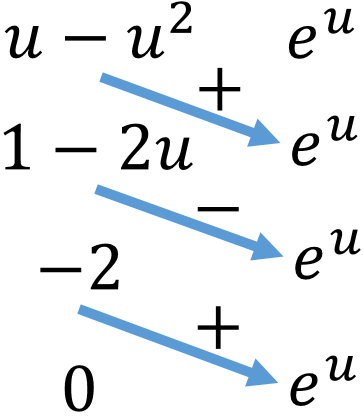
\includegraphics[width=30mm]{ibp_hw11.png}
\end{figure}
بنابراین
\eqn{
E\{X\}&=\int_0^1 (u-u^2)e^{u}du
\\&=(u-u^2)e^{u}-(1-2u)e^{u}+(-2)e^u\Big|_0^1=3-e
}
همچنین
\eqn{
E\{XY\}&=\int_0^1\int_x^1 xye^{1-x}dydx
\\&=\int_0^1 x(1-{x^2\over 2})e^{1-x}dx=6-2e
}

ت) X و Y، دو متغیر تصادفی گسسته (با مقادیر صحیح) اند و pmf آنها به صورت زیر است:
$
p_{X,Y}(x,y)=\begin{cases}
\frac{1}{16}&,\quad x^2+y^2\le 10 \ \ ,\ \ x\ge y\\
0&,\quad \text{سایر جاها}
\end{cases}
$
(در صورت سوال، مقدار $1\over 16$ باید به $1\over 21$ تغییر پیدا کند!)

جدول pmf به صورت زیر است ($p=21$):
\begin{figure}[htbp]
\centering
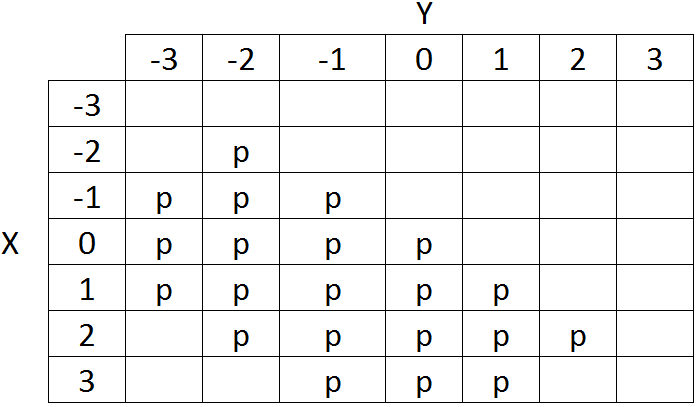
\includegraphics[width=80mm]{hw11_pmf.png}
\end{figure}

در این صورت:
\eqn{
&\Pr\{X=x\}=\begin{cases}
{1\over 21}&,\quad x=-2\\
{1\over 7}&,\quad x=-1\\
{4\over 21}&,\quad x=0\\
{5\over 21}&,\quad x=1\\
{5\over 21}&,\quad x=2\\
{1\over 7}&,\quad x=3\\
\end{cases}
}

همچنین
\eqn{
E\{X\}=\sum_x x\cdot\Pr\{X=x\}={13\over 21}
}

\eqn{
E\{XY\}=\sum_{x,y} xy\Pr\{X=x,Y=y\}={5\over21}
}

سوال 2) الف) به وضوح 
\eqn{
&\mu_X=E\{X\}=p_3+p_4
\\&\mu_Y=E\{Y\}=p_2+p_4
}{}
در نتیجه
\eqn{
&\text{\lr{cov}}(X,Y)=E\{(X-\mu_X)(Y-\mu_Y)\}
\\&=E\{XY\}-\mu_X\mu_Y
\\&=p_4-(p_2+p_4)(p_3+p_4)
}{}
در نتیجه برای صفر بودن کوواریانس باید داشته باشیم 
$
p_4=(p_2+p_4)(p_3+p_4)
$
.

ب) شرط همبستگی که در قسمت قبلی به دست آمد. برای استقلال باید داشته باشیم:
\eqn{
&p_1=(p_1+p_3)(p_1+p_2)
\\&p_2=(p_1+p_2)(p_2+p_4)
\\&p_3=(p_1+p_3)(p_3+p_4)
\\&p_4=(p_2+p_4)(p_3+p_4)
}{}
%از جمع هر چهار معادله‌ی فوق نتیجه می شود:
%\eqn{
%&p_1+p_2+p_3+p_4=
%p_1^2+p_2^2+p_3^2+p_4^2
%\\&+2p_1p_2+2p_1p_3+2p_1p_4
%\\&+2p_2p_3+2p_2p_4+2p_3p_4
%\\&\implies 1=1
%}{}
%بنابراین این 4 معادله از هم مستقل نیستند و می توان هر یک از این 4 معادله را حذف کرد. با حذف معادله‌ی 1، به معادلات زیر می رسیم:
%\eqn{
%&p_2=(1-p_3-p_4)(p_2+p_4)
%\\&p_3=(1-p_2-p_4)(p_3+p_4)
%\\&p_4=(p_2+p_4)(p_3+p_4)
%}{}
%از دو معادله‌ی اوب 
نکته اینجاست که
\begin{enumerate}
\item
از معادله‌ی 4، با کم کردن 
$
p_2+p_4
$
 به معادله‌ی 2 می رسیم.
\item
از معادله‌ی 4، با کم کردن 
$
p_3+p_4
$
 به معادله‌ی 3 می رسیم.
\item
از جمع معادله‌های 2، 3 و 4 به معادله‌ی 1 می رسیم.
\end{enumerate}
بنابراین در این سوال، 
\textbf{
ناهمبستگی و استقلال معادلند.
}
\newline\newline
سوال 3) الف) به سادگی و با انتگرال گیری می توان نتیجه گرفت:
\eqn{
&f_X(x)=\begin{cases}
1&,\quad 0<x<1
\\0&,\quad \text{در غیر این صورت}
\end{cases}
\\&f_Y(y)=\begin{cases}
1&,\quad 0<y<1
\\0&,\quad \text{در غیر این صورت}
\end{cases}
}{}
در نتیجه
\eqn{
E\{X\}=E\{Y\}={1\over 2}
}{}
هم چنین می دانیم
\eqn{
E\{XY\}&=\int_0^1\int_0^1 xy+\alpha xy\sin[2\pi(x+y)]dxdy
\\&={1\over 4}+\alpha\int_0^1\int_0^1 xy\sin[2\pi(x+y)]dxdy
\\&={1\over 4}+\alpha\int_0^1y\int_0^1 x\sin[2\pi(x+y)]dxdy
}{}
هم چنین
\eqn{
\int_0^1 x\sin[2\pi(x+y)]dx&=\left[-{x\over 2\pi}\cos[2\pi(x+y)]+{1\over 4\pi^2}\sin[2\pi(x+y)]\right]_{x=0}^{x=1}
\\&=-{\cos 2\pi y\over 2\pi}
}{}
در نتیجه
\eqn{
E\{XY\}&=
{1\over 4}-{\alpha\over 2\pi}\int_0^1y{\cos 2\pi y}dy
\\&={1\over 4}-{\alpha\over 2\pi}\left[{y\sin 2\pi y\over 2\pi}+{\cos 2\pi y\over 4\pi^2}\right]_{y=0}^{y=1}
\\&={1\over 4}
}{}
از آنجا که همواره 
$
E\{XY\}=E\{X\}E\{Y\}
$
، در نتیجه همواره دو متغیر تصادفی $X$ و $Y$ ناهمبسته هستند.

ب) به سادگی دیده می شود که 
$$
f_{X,Y}(x,y)=f_X(x)f_Y(y)\iff \alpha=0
$$

سوال 4) الف) با توجه به اینکه 
$
\Pr\{XY>1\}=0
$
 ، برای $u<1$ خواهیم داشت:
\eqn{
&\Pr\{XY<u\}=\Pr\left\{X<{u\over Y}\right\}
\\&=\int_{-\infty}^\infty \Pr\left\{X<{u\over y}|Y=y\right\}f_Y(y)dy
\\&=\int_0^1 \Pr\left\{X<{u\over y}|Y=y\right\}dy
\\&=\int_0^u \Pr\left\{X<{u\over y}\right\}dy
\\&+
\int_u^1 \Pr\left\{X<{u\over y}\right\}dy
\\&=u+\int_u^1 {u\over y}dy
\\&=u-u\ln u
}{}
بنابراین
\eqn{
f_{XY}(u)={d\over du}F_{XY}(u)=
\begin{cases}
-\ln u&,\quad 0\le u<1
\\0&,\quad \text{\rl{در غیر این صورت}}
\end{cases}
}{}
ب) ابتدا، می دانیم
\eqn{
\Pr\{X+Y<0\}=1-\Pr\{X+Y<2\}=0
}{}
بنابراین با فرض 
$
0<u<2
$
 خواهیم داشت:
\eqn{
&\Pr\{X+Y<u\}=\Pr\left\{X<{u-Y}\right\}
\\&=\int_{-\infty}^\infty \Pr\left\{X<{u-y}|Y=y\right\}f_Y(y)dy
\\&=\int_0^1 \Pr\left\{X<{u-y}|Y=y\right\}dy
%\\&=\int_0^u \Pr\left\{X<{u-y}\right\}dy
%\\&+
%\int_u^1 \Pr\left\{X<{u\over y}\right\}dy
%\\&=u+\int_u^1 {u\over y}dy
%\\&=u-u\ln u
}{}
به ازای $u<1$:
\eqn{
&\int_0^1 \Pr\left\{X<{u-y}|Y=y\right\}dy\\&=\int_0^u \Pr\left\{X<{u-y}|Y=y\right\}dy
\\&=\int_0^u u-ydy\\&={u^2\over 2}
}{}
به ازای $u>1$:
\eqn{
&\int_0^1 \Pr\left\{X<{u-y}|Y=y\right\}dy\\&=\int_{u-1}^1 \Pr\left\{X<{u-y}|Y=y\right\}dy
\\&+
\int_0^{u-1} \Pr\left\{X<{u-y}|Y=y\right\}dy
\\&=\int_{u-1}^1 u-ydy\\&+u-1
\\&=u(2-u)-{1\over 2}+{(u-1)^2\over 2}+u-1
\\&=2u-{u^2\over 2}
}{}
بنابراین
\eqn{
f(x)=
\begin{cases}
x&,\quad 0<x<1
\\2-x&,\quad 1\le x<2
\\0&,\quad\text{\rl{در غیر این صورت}}
\end{cases}
}{}
پ) به ازای $u>0$
\eqn{
&\Pr\left\{{X\over Y}<u\right\}=\Pr\left\{X<uY\right\}
\\&=\int_{-\infty}^\infty \Pr\left\{X<uy|Y=y\right\}f_Y(y)dy
\\&=\int_0^1 \Pr\left\{X<uy|Y=y\right\}dy
%\\&=\int_0^u \Pr\left\{X<{u-y}\right\}dy
%\\&+
%\int_u^1 \Pr\left\{X<{u\over y}\right\}dy
%\\&=u+\int_u^1 {u\over y}dy
%\\&=u-u\ln u
}{}
به ازای $u<1$ با اندکی محاسبات
\eqn{
\Pr\left\{{X\over Y}<u\right\}={u\over 2}
}{}
به ازای $u>1$ با اندکی محاسبات بیشتر
\eqn{
\Pr\left\{{X\over Y}<u\right\}=1-{1\over 2u}
}{}
بنابراین
\eqn{
f(x)=
\begin{cases}
{1\over 2}&,\quad 0<x<1
\\{1\over 2x^2}&,\quad 1\le x
\\0&,\quad\text{\rl{در غیر این صورت}}
\end{cases}
}{}
ت) با فرض 
$
0<u<1
$
 خواهیم داشت:
\eqn{
&\Pr\left\{\max\{X,Y\}<u\right\}=\Pr\left\{X<u,Y<u\right\}
\\&=\Pr\left\{X<u\right\}\Pr\left\{Y<u\right\}
=u^2
}{}
بنابراین
\eqn{
f(x)=
\begin{cases}
2x&,\quad 0<x<1
\\0&,\quad\text{\rl{در غیر این صورت}}
\end{cases}
}{}
ث) با فرض 
$
0<u<1
$
 خواهیم داشت:
\eqn{
&\Pr\left\{\min\{X,Y\}<u\right\}=1-\Pr\left\{\min\{X,Y\}>u\right\}
\\&=1-\Pr\left\{X>u,Y>u\right\}
\\&=1-\Pr\left\{X>u\right\}\Pr\left\{Y>u\right\}
=1-(1-u)^2
}{}
بنابراین
\eqn{
f(x)=
\begin{cases}
2-2x&,\quad 0<x<1
\\0&,\quad\text{\rl{در غیر این صورت}}
\end{cases}
}{}
اکنون اگر متغیرهای تصادفی $X$ و $Y$، نمایی با پارامتر 1 باشند، در این صورت با فرض 
$
u>0
$

ب)
\eqn{
&\Pr\left\{X+Y<u\right\}=\Pr\left\{X<u-Y\right\}
\\&=\int_0^\infty e^{-y}\Pr\left\{X<u-y\right\}dy
\\&=\int_0^u e^{-y}\Pr\left\{X<u-y\right\}dy
\\&=\int_0^u e^{-y}(1-e^{y-u})dy
\\&=\int_0^u e^{-y}-e^{-u}dy
\\&=1-e^{-u}-ue^{-u}
}{}
در نتیجه
\eqn{
f(x)=xe^{-x}\quad,\quad x>0
}{}
پ)
\eqn{
&\Pr\left\{{X\over Y}<u\right\}=\Pr\left\{X<uY\right\}
\\&=\int_0^\infty e^{-y}\Pr\left\{X<uy\right\}dy
%\\&=\int_0^u e^{-y}\Pr\left\{X<u-y\right\}dy
\\&=\int_0^\infty e^{-y}(1-e^{-yu})dy
\\&=\int_0^\infty e^{-y}-e^{-(1+u)y}dy
\\&=1-{1\over u+1}
}{}
در نتیجه
\eqn{
f(u)={1\over (u+1)^2}
\quad,\quad u>0
}{}

سوال 1)
\eqn{
F_X(x|X<1)&=\Pr\{X\le x|X<1\}
\\&={\Pr\{X\le x,x<1\}\over \Pr\{X<1\}}
\\&=\begin{cases}
{\Pr\{X\le x\}\over \Pr\{X<1\}}&,\quad 0<x<1\\
{\Pr\{X<1\}\over \Pr\{X<1\}}&,\quad x\ge1\\
\end{cases}
\\&=\begin{cases}
{{x\over 2}\over {1\over 2}}&,\quad 0<x<1\\
1&,\quad x\ge1\\
\end{cases}
\\&=\begin{cases}
x&,\quad 0<x<1\\
1&,\quad x\ge1\\
\end{cases}
}
همچنین
\eqn{
F_X(x|X>1)&=\Pr\{X\le x|X>1\}
\\&={\Pr\{X\le x,x>1\}\over \Pr\{X>1\}}
\\&=\begin{cases}
0&,\quad 0<x<1\\
{\Pr\{1<X< x\}\over \Pr\{X>1\}}&,\quad x\ge1\\
\end{cases}
\\&=\begin{cases}
0&,\quad 0<x<1\\
{{x-1\over 2}\over {1\over 2}}&,\quad x\ge1\\
\end{cases}
\\&=\begin{cases}
0&,\quad 0<x<1\\
x-1&,\quad 1<x<2\\
\end{cases}
}
بنابراین
\eqn{
f_X(x|X>1)&={d\over dx}F_X(x|X>1)
\\&=
\begin{cases}
1&,\quad 1<x<2\\
0&,\quad\text{سایر جاها}
\end{cases}
}

بسادگی از محاسبات (و همچنین شهود) می توان نتیجه گرفت که چون $X$ دارای توزیع یکنواخت بین 0 و 2 است، 
$
X|0.5<X<1.5
$
دارای توزیع یکنواخت بین 
$
0.5
$
و
$
1.5
$
خواهد بود. بنابراین واضح است که مقدار متوسط این متغیر تصادفی برابر 1 خواهد بود.

سوال 2) توزیع $X|X>a$ عبارتست از
\eqn{
F(x|X>a)&=\Pr\{X\le x|X>a\}
\\&={\Pr\{X\le x,X>a\}\over \Pr\{X>a\}}
\\&=
\begin{cases}
{\Pr\{X\le x,X>a\}\over \Pr\{X>a\}} &,\quad x>a\\
0&,\quad x<a
\end{cases}
\\&=
\begin{cases}
{e^{-\lambda a}-e^{-\lambda x}\over e^{-\lambda a}} &,\quad x>a\\
0&,\quad x<a
\end{cases}
\\&=
\begin{cases}
{1-e^{-\lambda (x-a)}} &,\quad x>a\\
0&,\quad x<a
\end{cases}
}
بنابراین
\eqn{
f(x|X>a)=
\begin{cases}
{\lambda e^{-\lambda (x-a)}} &,\quad x>a\\
0&,\quad x<a
\end{cases}
}
بنابراین
\eqn{
E\{X|X>a\}&=\int xf(X|X>a)dx
\\&=\int_a^\infty {\lambda xe^{-\lambda (x-a)}}dx
\\&=\int_a^\infty {\lambda (x-a+a)e^{-\lambda (x-a)}}dx
\\&=\int_0^\infty {\lambda (u+a)e^{-\lambda u}}du
\\&=\int_0^\infty {(\lambda u+\lambda a)e^{-\lambda u}}du
\\&=\int_0^\infty {\lambda ue^{-\lambda u}}du
+\int_0^\infty \lambda ae^{-\lambda u}du
\\&={1\over\lambda}
+a
}

همچنین
\eqn{
E\{X\}&=\int xf(x)dx
\\&=\int_0^\infty {\lambda xe^{-\lambda x}}dx
\\&={1\over\lambda}
}

این نشان می دهد
$$
E\{X|X>a\}=E\{X\}+a
$$
که همان خاصیت بی حافظه بودن متغیرهای نمایی است؛ به این معنا که تفاوتی نمیکند این متغیر از چه لحظه ای به بعد مشاهده شود. از هر لحظه ای به بعد، معادل با مشاهده آن در لحظه صفر خواهد بود.

سوال 3) الف) ابتدا توزیع 
$
X|X\ge 4
$
را می یابیم. بدین منظور:
\eqn{
p(x|X\ge4)&=\Pr\{X= x|X\ge 4\}
\\&={\Pr\{X= x,X\ge 4\}\over \Pr\{X\ge 4\}}
\\&=
\begin{cases}
{\Pr\{X= x\}\over \Pr\{X\ge 4\}}&,\quad x\ge 4\\
0&,\quad x< 4
\end{cases}
\\&=
\begin{cases}
{\Pr\{X=x\}\over (1-p)^4}&,\quad x\ge 4\\
0&,\quad x< 4
\end{cases}
\\&=
\begin{cases}
{(1-p)^xp\over (1-p)^4}&,\quad x\ge 4\\
0&,\quad x< 4
\end{cases}
\\&=
\begin{cases}
{(1-p)^{x-4}p}&,\quad x\ge 4\\
0&,\quad x<4
\end{cases}
}
بنابراین داریم

\eqn{
E\{X|X\ge 4\}&=\sum_{x=4}^\infty x(1-p)^{x-4}p
\\&=\sum_{u+4=4}^\infty (u+4)(1-p)^up
\\&=4+\sum_{u=0}^\infty u(1-p)^up
\\&={1\over p}+3
}

و

\eqn{
E\{X^2|X\ge 4\}&=\sum_{x=4}^\infty x^2(1-p)^{x-4}p
\\&=\sum_{u+4=4}^\infty (u+4)^2(1-p)^up
\\&=\sum_{u=0}^\infty (u^2+8u+16)(1-p)^up
\\&=16+8({1\over p}-1)+{(1-p)(2-p)\over p^2}
\\&={16p^2+8p(1-p)+(1-p)(2-p)\over p^2}
\\&={16p^2+8p-8p^2+p^2-3p+2\over p^2}
\\&={9p^2+5p+2\over p^2}
}
و می توان نوشت

\eqn{
\text{var}(X|X\ge 4)&=E\{X^2|X\ge 4\}-E^2\{X|X\ge 4\}
\\&={9p^2+5p+2\over p^2}-{9p^2+6p+1\over p^2}\\&={1-p\over p^2}
}

ب)
\eqn{
\Pr\{X=x|\text{X زوج است}\}&=
{\Pr\{X=x , X=0,2,4,\cdots\}\over \Pr\{X=0,2,4,\cdots\}}
\\&
=\begin{cases}
{\Pr\{X=x\}\over \Pr\{X=0,2,4,\cdots\}}&,\quad \text{x زوج}\\
0&,\quad \text{x فرد}
\end{cases}
\\&
=\begin{cases}
{(1-p)^xp\over \sum_{u=0}^\infty(1-p)^{2u}p}&,\quad \text{x زوج}\\
0&,\quad \text{x فرد}
\end{cases}
\\&
=\begin{cases}
{(1-p)^x\over {1\over 1-(1-p)^2}}&,\quad \text{x زوج}\\
0&,\quad \text{x فرد}
\end{cases}
\\&
=\begin{cases}
{(1-p)^x-(1-p)^{x+2}}&,\quad \text{x زوج}\\
0&,\quad \text{x فرد}
\end{cases}
\\&
=\begin{cases}
{p(2-p)(1-p)^x}&,\quad \text{x زوج}\\
0&,\quad \text{x فرد}
\end{cases}
}

سوال 4) الف)
\eqn{
\Pr\{Y\ge 3\}&=\int_3^\infty f_Y(y)dy
\\&=\int_3^\infty \sum_{x=1}^6 f_{X,Y}(x,y)dy
\\&=\int_3^\infty \sum_{x=1}^6 f_x(x)f_{Y|X}(x,y)dy
\\&=\int_3^\infty \sum_{x=1}^6 {1\over 6}f_{Y|X}(x,y)dy
\\&={1\over 6}\int_3^\infty f_{Y|X}(1,y)dy
\\&+{1\over 6}\int_3^\infty f_{Y|X}(2,y)dy
\\&+{1\over 6}\int_3^\infty f_{Y|X}(3,y)dy
\\&+{1\over 6}\int_3^\infty f_{Y|X}(4,y)dy
\\&+{1\over 6}\int_3^\infty f_{Y|X}(5,y)dy
\\&+{1\over 6}\int_3^\infty f_{Y|X}(6,y)dy
\\&={1\over 6}({1\over 4}+{2\over 5}+{3\over 6})
\\&={23\over 120}
}

ب)
\eqn{
f_Y(y)&=\sum_x f_{X,Y}(x,y)
\\&=\sum_x f_x(x)f_{Y|X}(x,y)
\\&={1\over 6}\sum_{x=1}^6f_{Y|X}(x,y)
\\&={1\over 6}\times\begin{cases}
1+{1\over 2}+{1\over 3}+{1\over 4}+{1\over 5}+{1\over 6}&,\quad 0<y<1\\
{1\over 2}+{1\over 3}+{1\over 4}+{1\over 5}+{1\over 6}&,\quad 1<y<2\\
{1\over 3}+{1\over 4}+{1\over 5}+{1\over 6}&,\quad 2<y<3\\
{1\over 4}+{1\over 5}+{1\over 6}&,\quad 3<y<4\\
{1\over 5}+{1\over 6}&,\quad 4<y<5\\
{1\over 6}&,\quad 5<y<6\\
\end{cases}
\\&=\begin{cases}
{49\over 120}&,\quad 0<y<1\\
{29\over 120}&,\quad 1<y<2\\
{19\over 120}&,\quad 2<y<3\\
{37\over 360}&,\quad 3<y<4\\
{11\over 180}&,\quad 4<y<5\\
{1\over 36}&,\quad 5<y<6\\
\end{cases}
}

بنابراین
\eqn{
\mathbb{E}\{Y\}&=\int_0^6 yf_Y(y)dy
\\&=\cdots(!!!)
\\&=1.75
}

\eqn{
\mathbb{E}\{Y^2\}&=\int_0^6 y^2f_Y(y)dy
\\&=\cdots(!!!)
\\&\approx5.06
}
بنابراین
$$
\text{var}(Y)\approx2
$$

\QA

ابتدا باید 
$
f_X(x|X\ge 1)
$
را محاسبه کنیم. برای این منظور داریم:
\eqn{
\Pr\{X\le x|X\ge 1\}&=\frac{\Pr\{1\le X\le x\}}{\Pr\{X\ge 1\}}
\\&=\frac{\Pr\{1\le X\le x\}}{\Pr\{X=1\}}
\\&=\frac{\Pr\{1\le X\le x\}}{\frac{1}{2}}
\\&=\begin{cases}
1&,\quad x\ge 1\\
0&,\quad x< 1
\end{cases}
}
در این صورت
$$
f_X(x|X\ge 1)=\delta(x-1)
$$
و خواهیم داشت
\eqn{
E\{X|X\ge 1\}&=\int_{-\infty}^\infty xf_X(x|X\ge 1)dx
\\&=\int_{-\infty}^\infty x\delta(x-1)dx=1
}
\eqn{
E\{X^2|X\ge 1\}&=\int_{-\infty}^\infty x^2f_X(x|X\ge 1)dx
\\&=\int_{-\infty}^\infty x^2\delta(x-1)dx=1
}
بنابراین
\eqn{
E\{X|X\ge 1\}=1\quad,\quad
\sigma^2(X|X\ge 1)=E\{X^2|X\ge 1\}-E^2\{X|X\ge 1\}=0
}

برای چگالی احتمال زیر، مقادیر
$
\mathbb{E}\{X|X>1\}
$
و
$
\sigma_X^2(X|X>1)
$
برای محاسبه‌ی
$
f(x|X\ne 1)
$
داریم
\eqn{
\Pr\{X\le x|X\ne 1\}&=\frac{\Pr\{X\le x,X\ne 1\}}{\Pr\{X\ne 1\}}
\\&=\frac{\Pr\{X\le x,X\ne 1\}}{\frac{1}{2}}
\\&=
\begin{cases}
\frac{\Pr\{X<1\}}{\frac{1}{2}}&,\quad x\ge 1\\
\frac{\Pr\{X\le x\}}{\frac{1}{2}}&,\quad x<1
\end{cases}
\\&=
\begin{cases}
1&,\quad x\ge 1\\
3x^2-2x^3&,\quad 0\le x<1\\
0&,\quad x<0
\end{cases}
}
در نتیجه
\eqn{
f_X(x|X\ne 1)=
\begin{cases}
6x-6x^2&,\quad 0<x< 1\\
0&,\quad \text{سایر جاها}
\end{cases}
}

در نهایت، برای محاسبه‌ی 
$
f(x|X<\frac{1}{2})
$
چنین می‌نویسیم:
\eqn{
\Pr\{X\le x|X<\frac{1}{2}\}&=
\frac{\Pr\{X\le x,X<\frac{1}{2}\}}{\Pr\{X<\frac{1}{2}\}}
\\&=
\begin{cases}
\frac{\Pr\{X<\frac{1}{2}\}}{\Pr\{X<\frac{1}{2}\}}&,\quad x\ge \frac{1}{2}\\
\frac{\Pr\{X\le x\}}{\Pr\{X<\frac{1}{2}\}}&,\quad x<\frac{1}{2}
\end{cases}
\\&=
\begin{cases}
1&,\quad x\ge \frac{1}{2}\\
6x^2-4x^3&,\quad 0\le x<\frac{1}{2}\\
0&,\quad x<0
\end{cases}
}
پس:
$$
f_X(x|X<\frac{1}{2})=
\begin{cases}
12x-12x^2&,\quad 0< x<\frac{1}{2}\\
0&,\quad \text{سایر جاها}
\end{cases}.
$$

\QA

الف) 

\eqn{
\Pr\{\max\{X,Y\}\le u|X\le \frac{1}{2}\}&=
\Pr\{X\le u,Y\le u|X\le \frac{1}{2}\}
\\&=
\frac{\Pr\{X\le u,Y\le u,X\le \frac{1}{2}\}}{\Pr\{X\le \frac{1}{2}\}}
\\&=
\begin{cases}
\frac{\Pr\{Y\le u,X\le \frac{1}{2}\}}{\Pr\{X\le \frac{1}{2}\}}&,\quad u\ge \frac{1}{2}\\
\frac{\Pr\{X\le u,Y\le u\}}{\Pr\{X\le \frac{1}{2}\}}&,\quad u< \frac{1}{2}
\end{cases}
}
از طرفی
\eqn{
\Pr\{X\le \frac{1}{2}\}&=\int_{x^2+y^2\le 1,x\le \frac{1}{2}}
\frac{1}{\pi}dxdy
\\&=
\frac{1}{\pi}\int_{x^2+y^2\le 1,x\le \frac{1}{2}}dxdy
\\&=\frac{\sqrt 3}{4\pi}+\frac{2}{3}.
}

همچنین
\eqn{
\Pr\{X\le \frac{1}{2},Y\le u\}&=
\int_{-1}^{\frac{1}{2}}
\int_{-\sqrt{1-x^2}}^{\min\{\sqrt{1-x^2},u\}}\frac{1}{\pi}dydx
\\&=
\frac{1}{\pi}
\int_{x\in(-1,\frac{1}{2}),u\ge -\sqrt{1-x^2}}
\min\{\sqrt{1-x^2},u\}+\sqrt{1-x^2}dx
\\&=
C_1+\frac{1}{\pi}
\int_{x\in(-1,\frac{1}{2}),u\ge -\sqrt{1-x^2}}
\min\{\sqrt{1-x^2},u\}dx
}
که در رابطه بالا، 
$
C_1=\frac{1}{\pi}
\int_{-1}^{\frac{1}{2}}
\sqrt{1-x^2}dx
$
(تعیین مقدار دقیق آن اهمیت ندارد؛ زیرا همانطور که بعدا دیده می‌شود، در مشتق گیری حذف خواهد شد.)

با مشتق گیری خواهیم داشت:
\eqn{
\frac{d}{du}
\Pr\{X\le \frac{1}{2},Y\le u\}
&=
\frac{1}{\pi}\int_{x\in(-1,\frac{1}{2}),-\sqrt{1-x^2}\le u\le \sqrt{1-x^2}}dx
\\&=
\begin{cases}
\frac{1}{\pi}\int_{x\in(-1,\frac{1}{2}),-\sqrt{1-x^2}\le u}dx&,\quad u\le 0\\
\frac{1}{\pi}\int_{x\in(-1,\frac{1}{2}),u\le \sqrt{1-x^2}}dx&,\quad u\ge 0
\end{cases}
\\&=
\frac{1}{\pi}\int_{x\in(-1,\frac{1}{2}),-\sqrt{1-u^2}<x<\sqrt{1-u^2}}dx
\\&=
\frac{1}{\pi}\min\left\{\sqrt{1-u^2},\frac{1}{2}\right\}+\frac{1}{\pi}\min\{\sqrt{1-u^2},1\}
}

به طریق مشابه

\eqn{
\frac{d}{du}
\Pr\{X\le u,Y\le u\}
&=
\frac{1}{\pi}\int_{x\in(-1,u),-\sqrt{1-x^2}\le u\le \sqrt{1-x^2}}dx
\\&=
\begin{cases}
\frac{1}{\pi}\int_{x\in(-1,u),-\sqrt{1-x^2}\le u}dx&,\quad u\le 0\\
\frac{1}{\pi}\int_{x\in(-1,u),u\le \sqrt{1-x^2}}dx&,\quad u\ge 0
\end{cases}
\\&=
\frac{1}{\pi}\int_{x\in(-1,u),-\sqrt{1-u^2}<x<\sqrt{1-u^2}}dx
\\&=
\frac{1}{\pi}\min\left\{\sqrt{1-u^2},u\right\}+\frac{1}{\pi}\min\{\sqrt{1-u^2},1\}
}
بنابراین
%\eqn{
%\Pr\{X\le u,Y\le u\}&=
%\int_{-1}^{u}
%\int_{-\sqrt{1-x^2}}^{\min\{\sqrt{1-x^2},u\}}\frac{1}{\pi}dydx
%\\&=
%\frac{1}{\pi}
%\int_{x\in(-1,u),u\ge -\sqrt{1-x^2}}
%\min\{\sqrt{1-x^2},u\}+\sqrt{1-x^2}dx
%\\&=
%C_1+\frac{1}{\pi}
%\int_{x\in(-1,u),u\ge -\sqrt{1-x^2}}
%\min\{\sqrt{1-x^2},u\}dx
%}

%\eqn{
%\Pr\{Y\le u\}=
%\begin{cases}
%1-\frac{1}{\pi}\cos^{-1}u+\frac{u}{\pi}\sqrt{1-u^2}&,\quad 0\le u\le 1\\
%\frac{1}{\pi}\cos^{-1}(-u)+\frac{u}{\pi}\sqrt{1-u^2}&,\quad -1\le u\le 0\\
%0&,\quad\text{سایر جاها}
%\end{cases}
%}
%و
%\eqn{
%\Pr\{Y\le u,X\ge \frac{1}{2}\}=
%\begin{cases}
%1-\frac{1}{\pi}\cos^{-1}u+\frac{u}{\pi}\sqrt{1-u^2}&,\quad u\ge 0\\
%\frac{1}{\pi}\cos^{-1}u+\frac{u}{\pi}\sqrt{1-u^2}&,\quad u<0\\
%\end{cases}
%}

\eqn{
f_{\max\{X,Y\}}(u|X\le \frac{1}{2})
&=
\begin{cases}
\frac{1}{\pi}\min\left\{\sqrt{1-u^2},\frac{1}{2}\right\}\\+
\frac{1}{\pi}\min\left\{\sqrt{1-u^2},u\right\}\\+
\frac{2}{\pi}\min\{\sqrt{1-u^2},1\}&,\quad |u|\le 1\\
0&,\quad |u|>1
\end{cases}
}

ب)

\eqn{
&\Pr\{\sqrt{X^2+Y^2}\le u|X+Y\le 1\}=
\frac{\Pr\{\sqrt{X^2+Y^2}\le u,X+Y\le 1\}}{\Pr\{X+Y\le 1\}}
\\&=
\frac{1}{\frac{3}{4}+\frac{1}{2\pi}}
\Pr\{\sqrt{X^2+Y^2}\le u,X+Y\le 1\}
\\&=
\begin{cases}
1&,\quad u\ge 1\\
\frac{1}{\frac{3}{4}+\frac{1}{2\pi}}
\left[(1-\frac{1}{\pi}\cos^{-1}\frac{1}{u\sqrt 2})u^2+\frac{1}{\pi}\sqrt{\frac{u^2}{2}-\frac{1}{4}}\right]&,\quad \frac{1}{\sqrt 2}\le u< 1\\
\frac{u^2}{\frac{3}{4}+\frac{1}{2\pi}}&,\quad 0\le u< \frac{1}{\sqrt 2}\\
0&,\quad u\le 0\\
\end{cases}
}
در نتیجه
\eqn{
&f_{\sqrt{X^2+Y^2}|X+Y\le 1}(u)=
\begin{cases}
\frac{2u}{\frac{3}{4}+\frac{1}{2\pi}}
(1-\frac{1}{\pi}\cos^{-1}\frac{1}{u\sqrt 2})&,\quad \frac{1}{\sqrt 2}\le u< 1\\
\frac{2u}{\frac{3}{4}+\frac{1}{2\pi}}&,\quad 0\le u< \frac{1}{\sqrt 2}\\
0&,\quad \text{سایر جاها}\\
\end{cases}
}
در نتیجه
\eqn{
\mathbb{E}\{\sqrt{X^2+Y^2}|X+Y\le 1\}
&=\int_0^1 uf_{\sqrt{X^2+Y^2}|X+Y\le 1}(u)du
\\&=
\int_0^{\frac{1}{\sqrt2}} \frac{2u^2}{\frac{3}{4}+\frac{1}{2\pi}}du
\\&+
\int_{\frac{1}{\sqrt2}}^1 \frac{2u^2}{\frac{3}{4}+\frac{1}{2\pi}}
(1-\frac{1}{\pi}\cos^{-1}\frac{1}{u\sqrt 2})du
\\&=
\int_0^1 \frac{2u^2}{\frac{3}{4}+\frac{1}{2\pi}}du
\\&-
\frac{2}{\frac{3\pi}{4}+\frac{1}{2}}\int_{\frac{1}{\sqrt2}}^1 u^2\cos^{-1}\frac{1}{u\sqrt 2}du
\\&=
\frac{2}{3}+\frac{\sqrt2}{9\pi+6}\ln(1+\sqrt 2)
%\\&=
%\frac{1}{\frac{3}{4}+\frac{1}{2\pi}}
%\left[
%\frac{1}{2}+\frac{1}{3\pi}+\frac{\sqrt 2}{12\pi}\ln(1+\sqrt 2)
%\right]
}
%
%
%
% مقدار 
%$
%\mathbb{E}\{\sqrt{X^2+Y^2}|X+Y\le 1\}
%$
%را بیابید.

\QA

الف)
\eqn{
\Pr\{Y\le 0|X=1\}&=
\int_{-\infty}^0 f(y|X=1)dy
\\&=
\int_{-\infty}^0 \frac{a}{2}\exp(-a|y-1|)dy
\\&=
\int_{-\infty}^0 \frac{a}{2}\exp(a(y-1))dy
=\frac{e^{-a}}{2}
}
و
\eqn{
\Pr\{Y\ge 0|X=-1\}&=
\int_{-\infty}^0 f(y|X=1)dy
\\&=
\int_0^\infty \frac{a}{2}\exp(-a|y+1|)dy
\\&=
\int_0^\infty \frac{a}{2}\exp(-a(y+1))dy
=\frac{e^{-a}}{2}
}
مشاهده می شود که هر دو احتمال، با افزایش مقدار $a$ افت می‌کنند.

ب) صورت سوال، یک مسئله‌ی مخابراتی را نشان می دهد که در آن، مقادیر $-1$ و $1$ روی کانال ارسال می‌شوند و نویزی با چگالی احتمال نمایی دوطرفه، با سیگنال ارسالی جمع می‌شود. هر چه $a$ بیشتر باشد، واریانس (توان) نویز کاهش می‌یابد و انتظار می‌رود که احتمال خطا در آشکارسازی سمبلهای ارسالی در گیرنده نیز کاهش یابد. این امر، با محاسبه‌ی احتمالهای 
$
\Pr\{Y\le 0|X=1\}
$
و
$
\Pr\{Y\ge 0|X=-1\}
$
تحقیق شد.

\chapter{دنباله‌ی متغیرهای تصادفی}






%کوئیز 10)
%$
%X
%$
%می تواند مقادیر 0 و 1 و 
%$
%Y
%$
%می تواند مقادیر 0، 2، 4 و 6 را اختیار کند. در نتیجه
%\eqn{
%\Pr\{X=2Y\}&=\Pr\{X=2Y=0\}+\Pr\{X=2Y=1\}
%\\&=\Pr\{X=0,Y=0\}+\Pr\{X=1,Y=\frac{1}{2}\}
%\\&=\Pr\{i<4,i\in\{1,3,5\}\}+0
%\\&=\Pr\{i\in\{1,3\}\}=\frac{1}{3}
%}




%کوئیز 10)
%$
%X
%$
%می تواند مقادیر 0 و 1 و 
%$
%Y
%$
%می تواند مقادیر 0، 2، 4 و 6 را اختیار کند. در نتیجه
%\eqn{
%\Pr\{X=2Y\}&=\Pr\{X=2Y=0\}+\Pr\{X=2Y=1\}
%\\&=\Pr\{X=0,Y=0\}+\Pr\{X=1,Y=\frac{1}{2}\}
%\\&=\Pr\{i<4,i\in\{1,3,5\}\}+0
%\\&=\Pr\{i\in\{1,3\}\}=\frac{1}{3}
%}


\end{document}